\begin{figure}[p]
    \centering
    \begin{subfigure}[b]{0.32\textwidth}
        \centering
        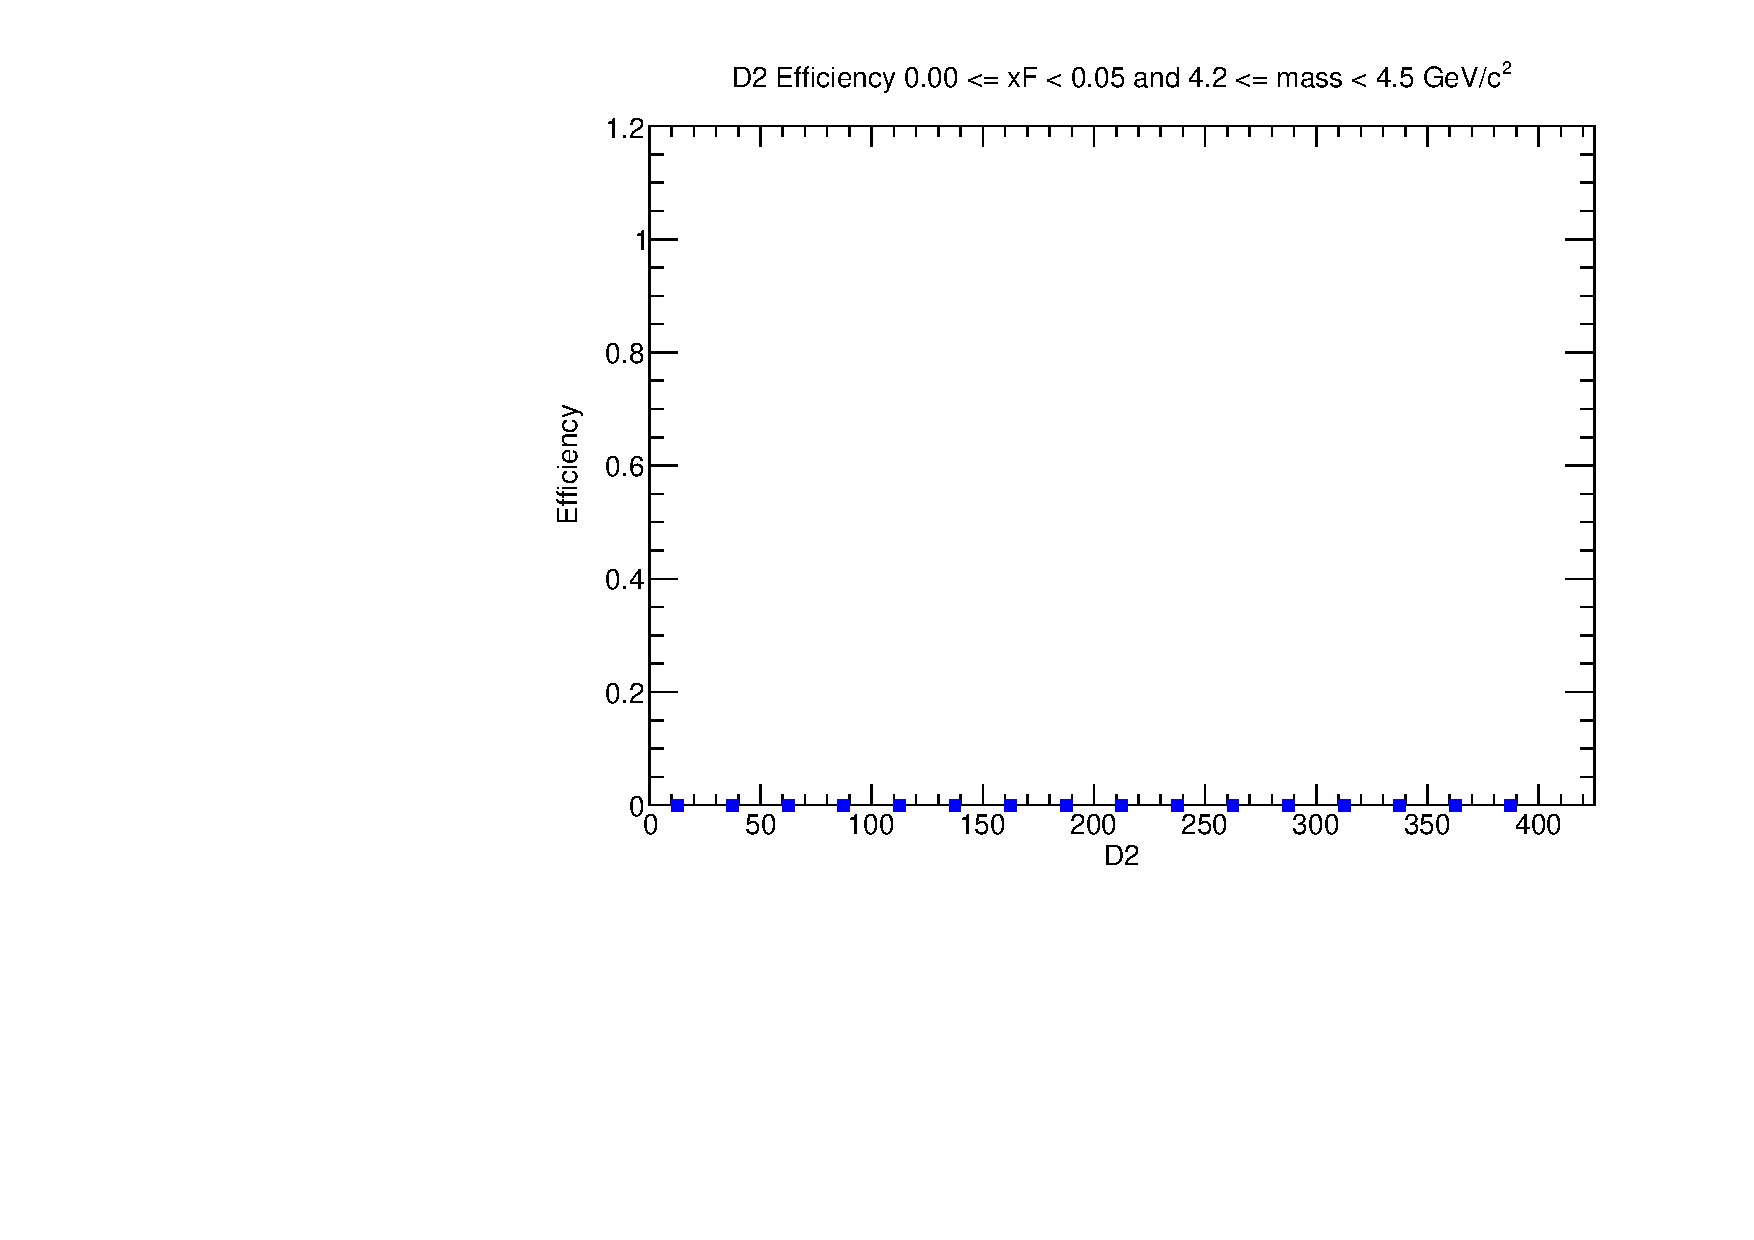
\includegraphics[width=\textwidth]{./kTrackerEfficiencyPlots/D2_Efficiency_xF0_mass0.pdf}
        \caption{$4.2 \leq m < 4.5$ GeV/$c^2$}
        \label{fig:xF0_mass0}
    \end{subfigure}
    \hfill
    \begin{subfigure}[b]{0.32\textwidth}
        \centering
        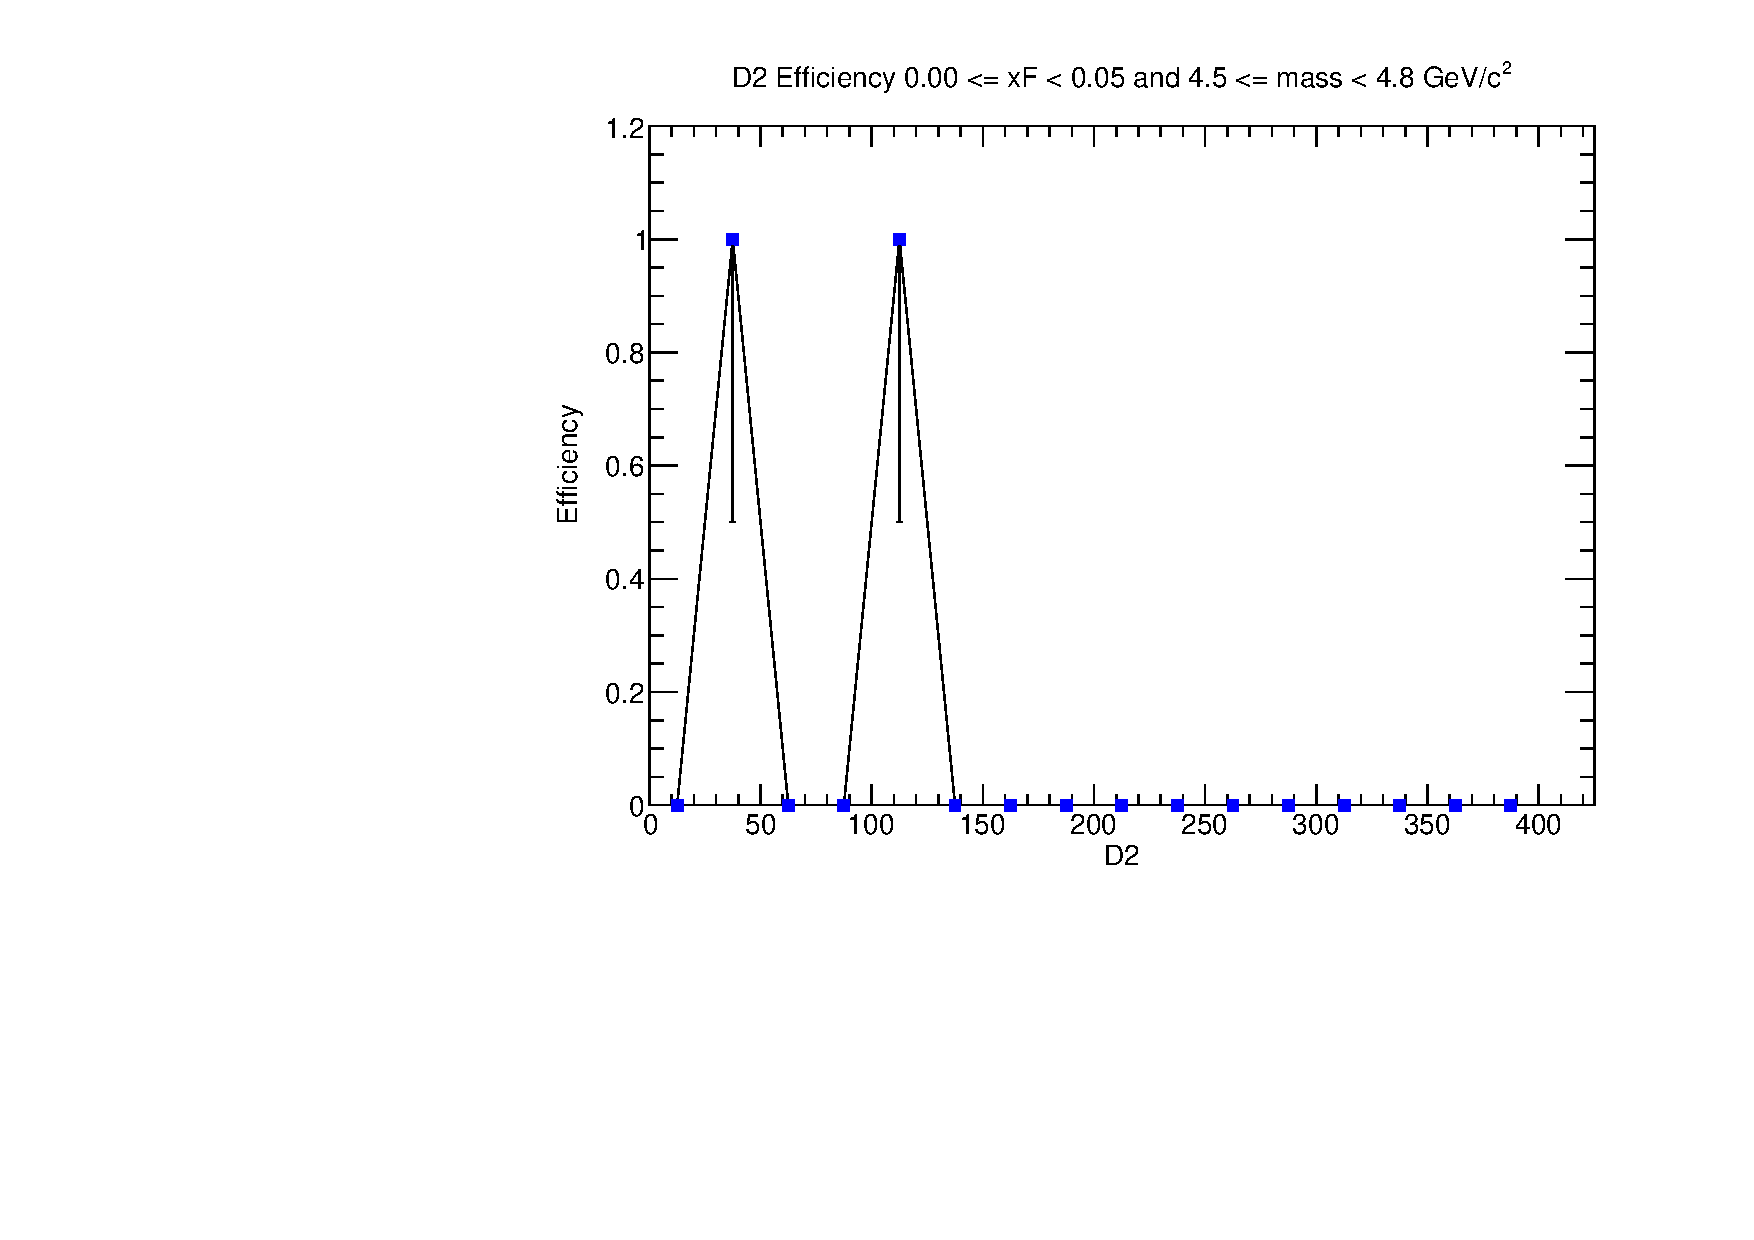
\includegraphics[width=\textwidth]{./kTrackerEfficiencyPlots/D2_Efficiency_xF0_mass1.pdf}
        \caption{$4.5 \leq m < 4.8$ GeV/$c^2$}
        \label{fig:xF0_mass1}
    \end{subfigure}
    \hfill
    \begin{subfigure}[b]{0.32\textwidth}
        \centering
        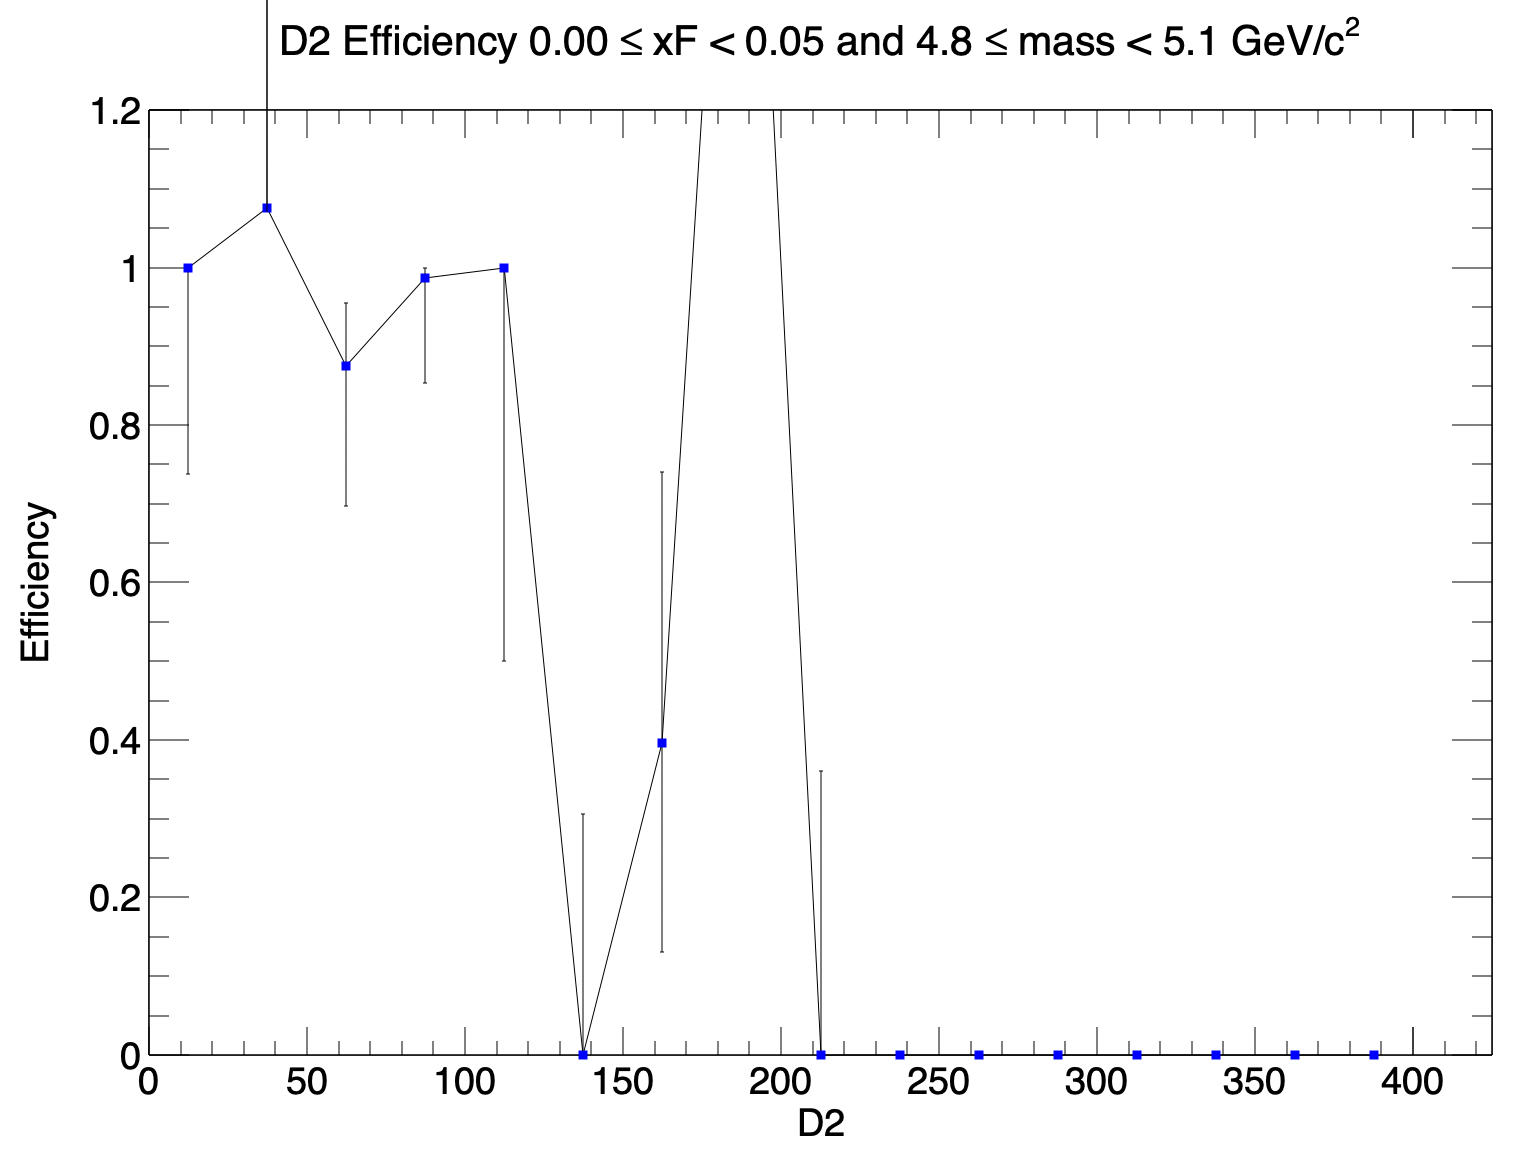
\includegraphics[width=\textwidth]{./kTrackerEfficiencyPlots/D2_Efficiency_xF0_mass2.png}
        \caption{$4.8 \leq m < 5.1$ GeV/$c^2$}
        \label{fig:xF0_mass2}
    \end{subfigure}
    \vspace{0.5cm}
    \begin{subfigure}[b]{0.32\textwidth}
        \centering
        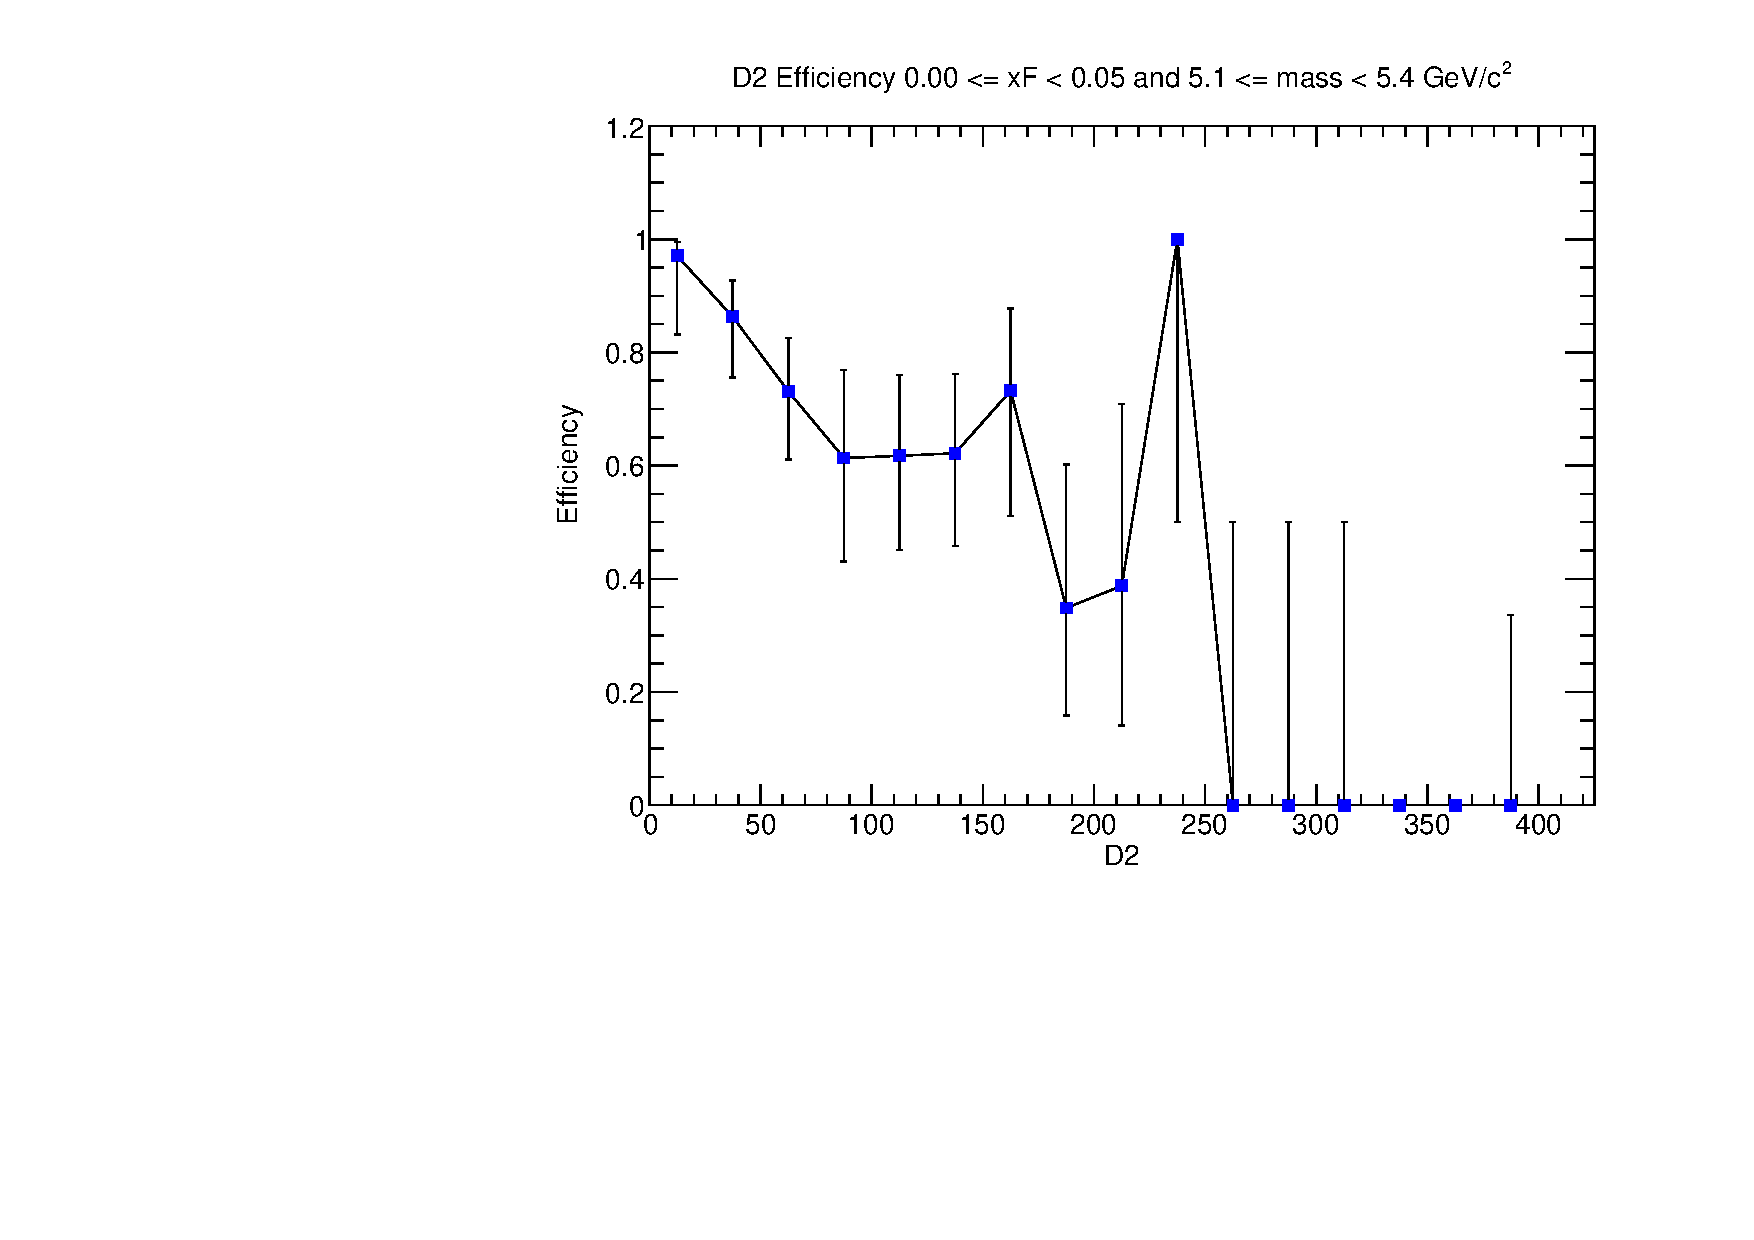
\includegraphics[width=\textwidth]{./kTrackerEfficiencyPlots/D2_Efficiency_xF0_mass3.pdf}
        \caption{$5.1 \leq m < 5.4$ GeV/$c^2$}
        \label{fig:xF0_mass3}
    \end{subfigure}
    \hfill
    \begin{subfigure}[b]{0.32\textwidth}
        \centering
        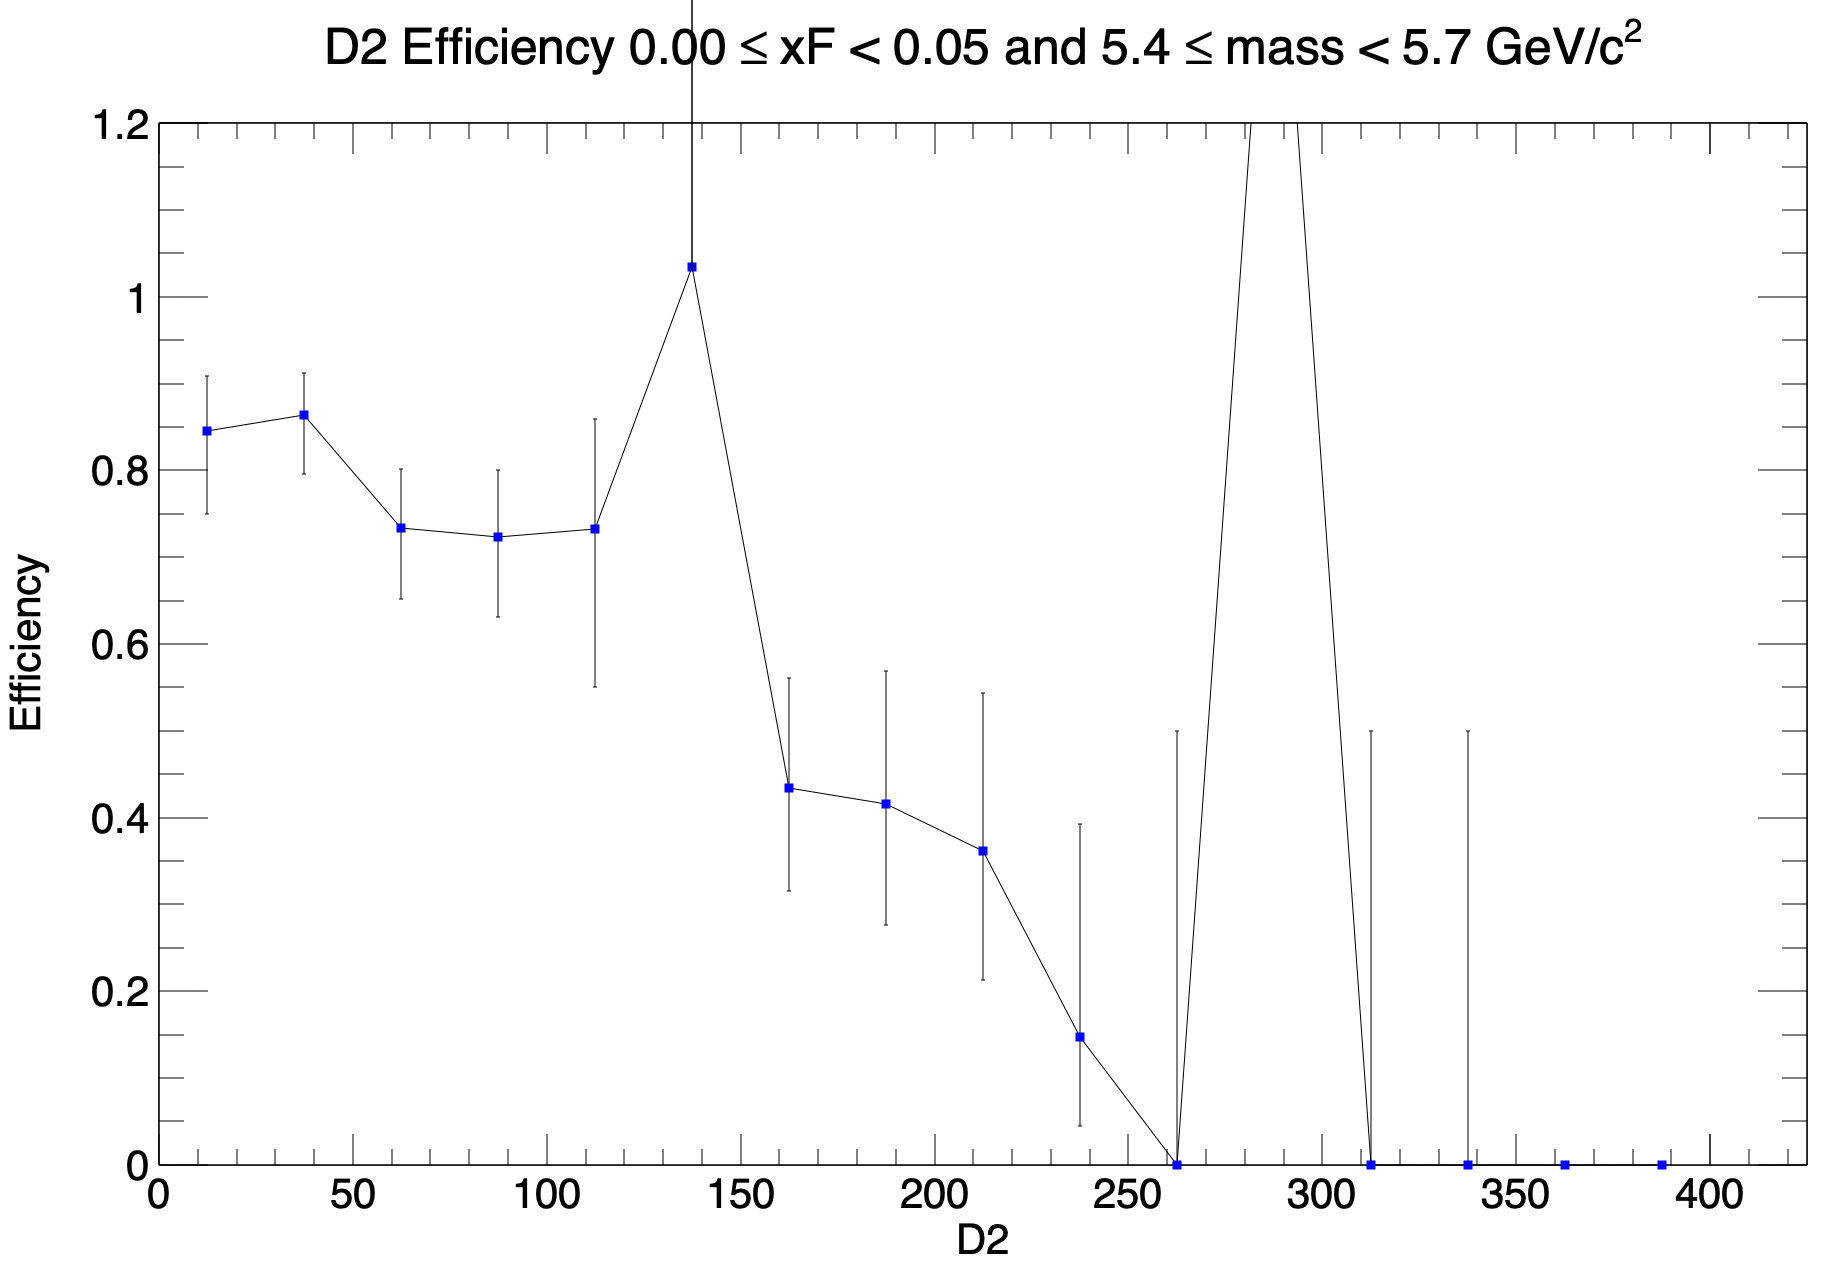
\includegraphics[width=\textwidth]{./kTrackerEfficiencyPlots/D2_Efficiency_xF0_mass4.png}
        \caption{$5.4 \leq m < 5.7$ GeV/$c^2$}
        \label{fig:xF0_mass4}
    \end{subfigure}
    \hfill
    \begin{subfigure}[b]{0.32\textwidth}
        \centering
        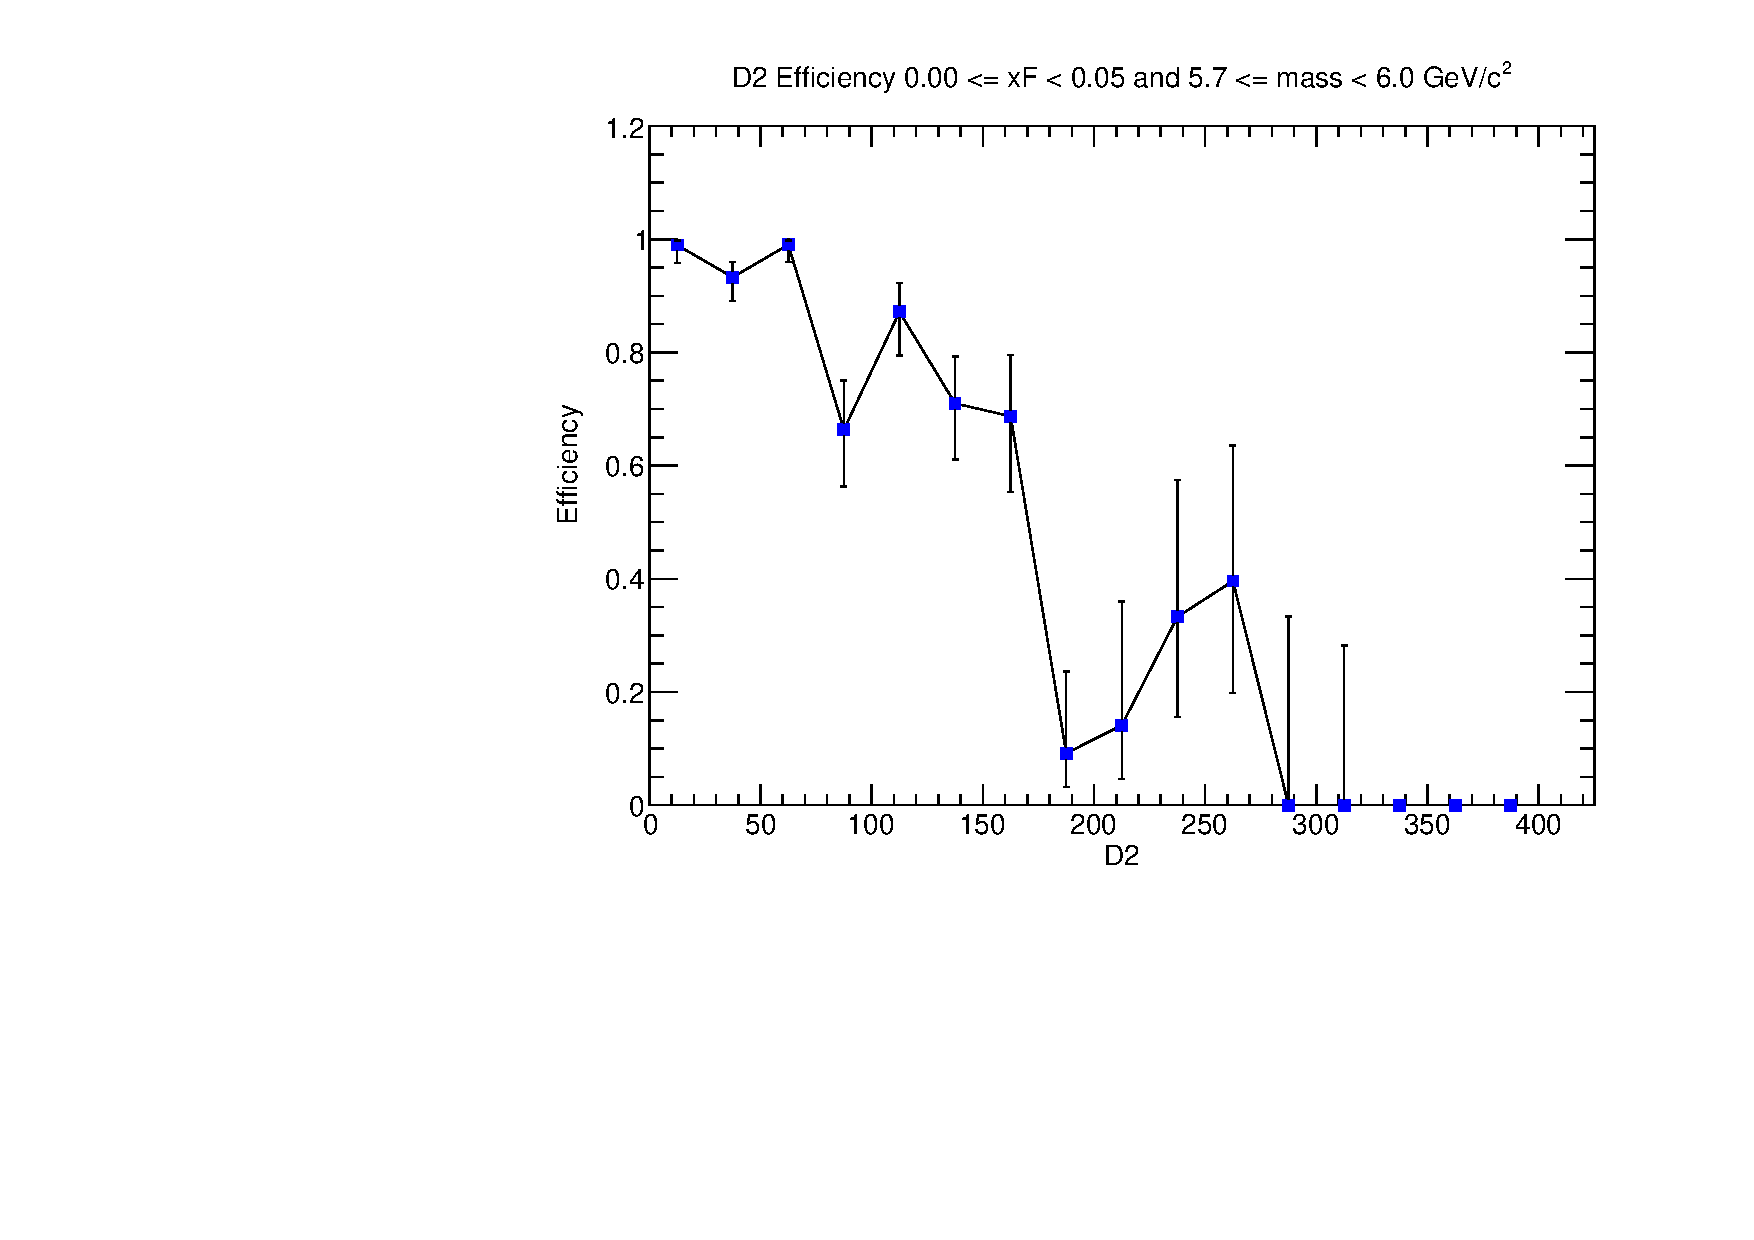
\includegraphics[width=\textwidth]{./kTrackerEfficiencyPlots/D2_Efficiency_xF0_mass5.pdf}
        \caption{$5.7 \leq m < 6.0$ GeV/$c^2$}
        \label{fig:xF0_mass5}
    \end{subfigure}
    \vspace{0.5cm}
    \begin{subfigure}[b]{0.32\textwidth}
        \centering
        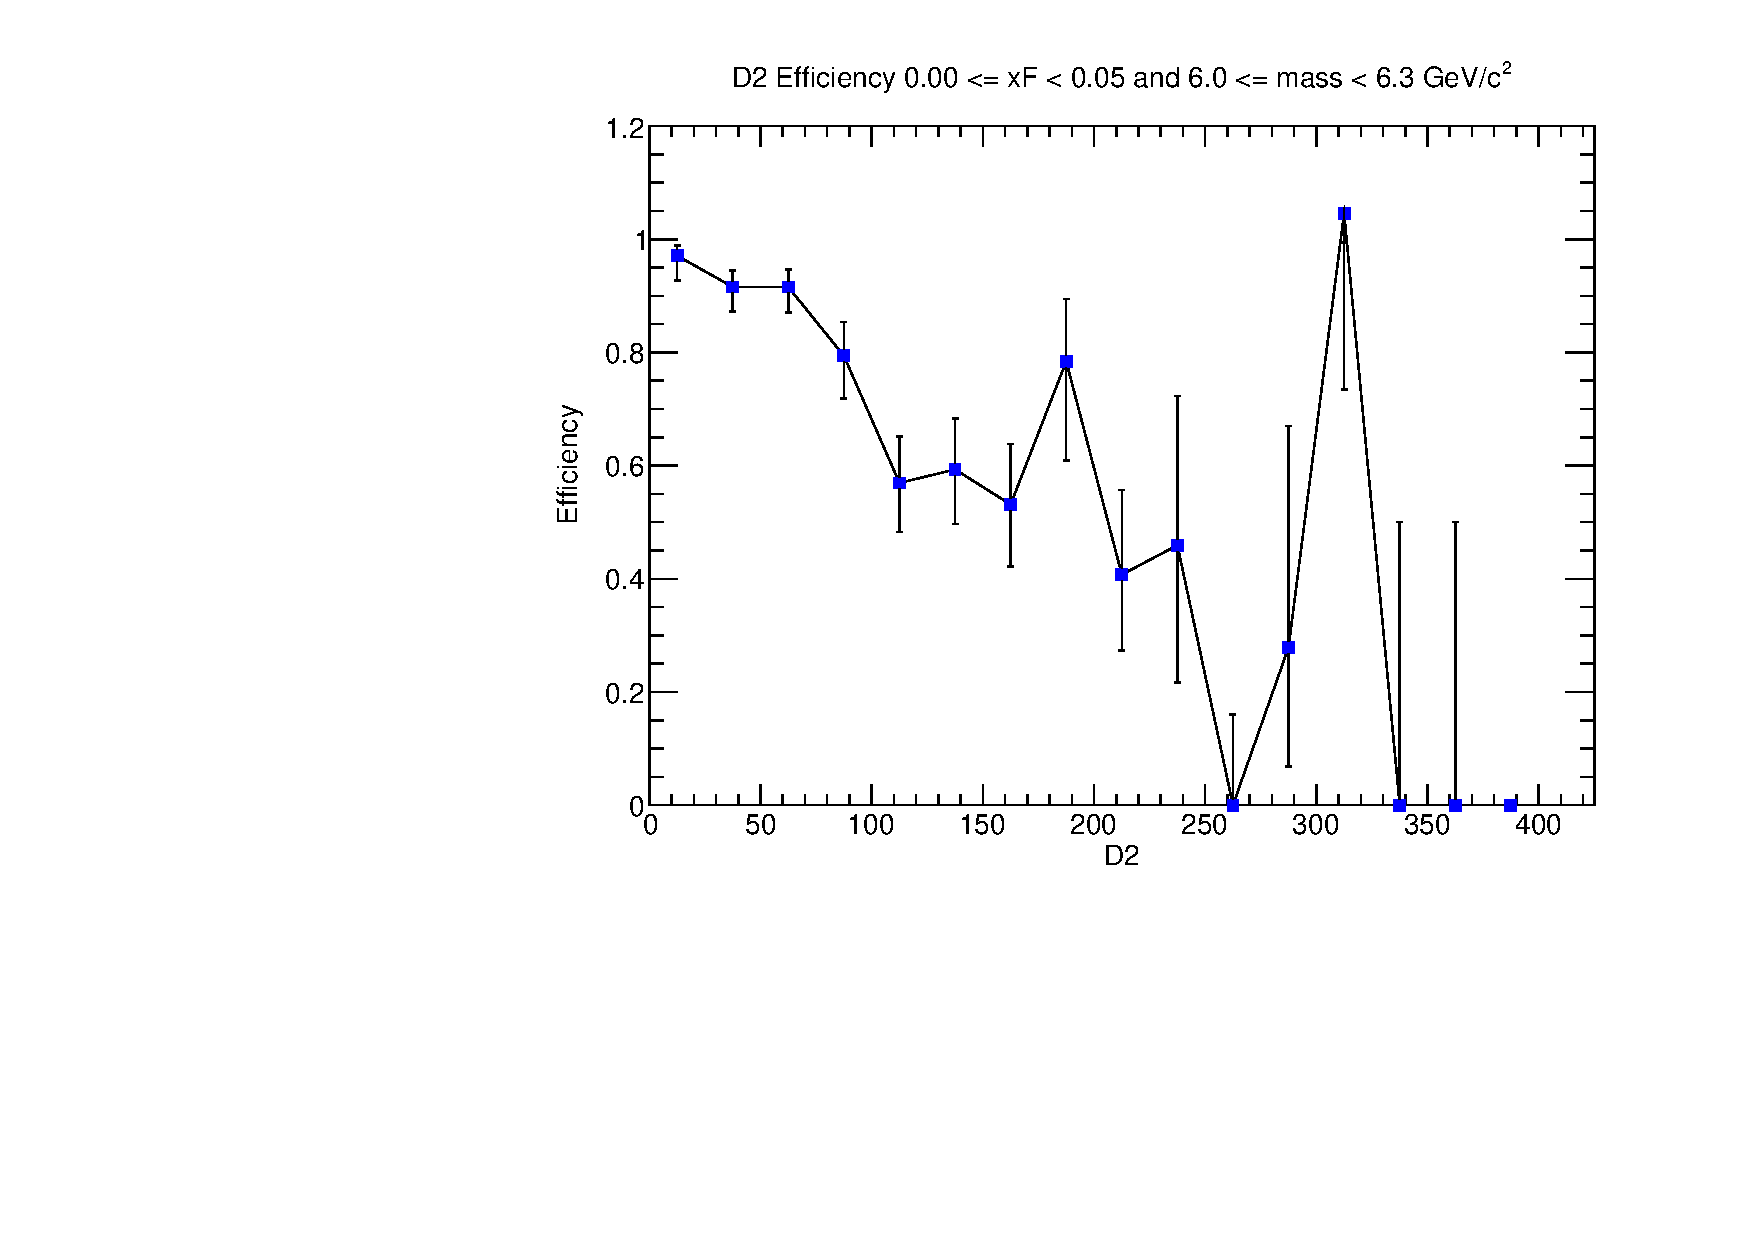
\includegraphics[width=\textwidth]{./kTrackerEfficiencyPlots/D2_Efficiency_xF0_mass6.pdf}
        \caption{$6.0 \leq m < 6.3$ GeV/$c^2$}
        \label{fig:xF0_mass6}
    \end{subfigure}
    \hfill
    \begin{subfigure}[b]{0.32\textwidth}
        \centering
        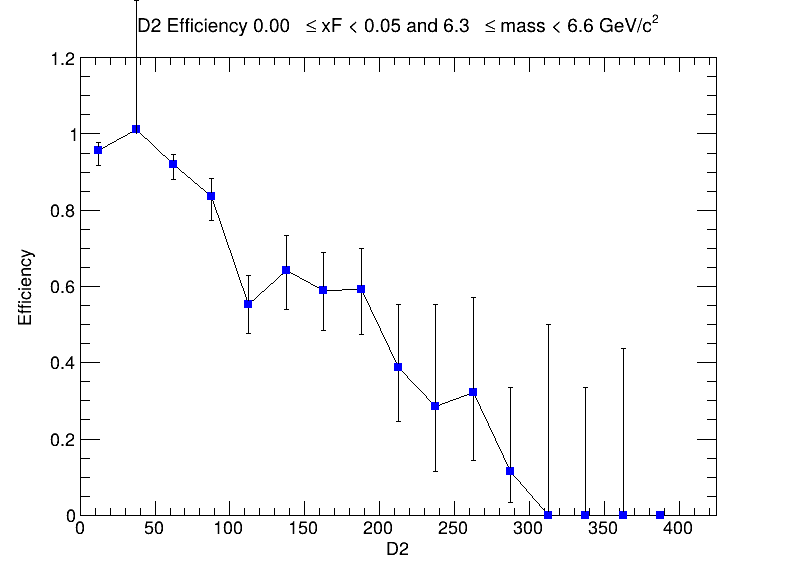
\includegraphics[width=\textwidth]{./kTrackerEfficiencyPlots/D2_Efficiency_xF0_mass7.png}
        \caption{$6.3 \leq m < 6.6$ GeV/$c^2$}
        \label{fig:xF0_mass7}
    \end{subfigure}
    \hfill
    \begin{subfigure}[b]{0.32\textwidth}
        \centering
        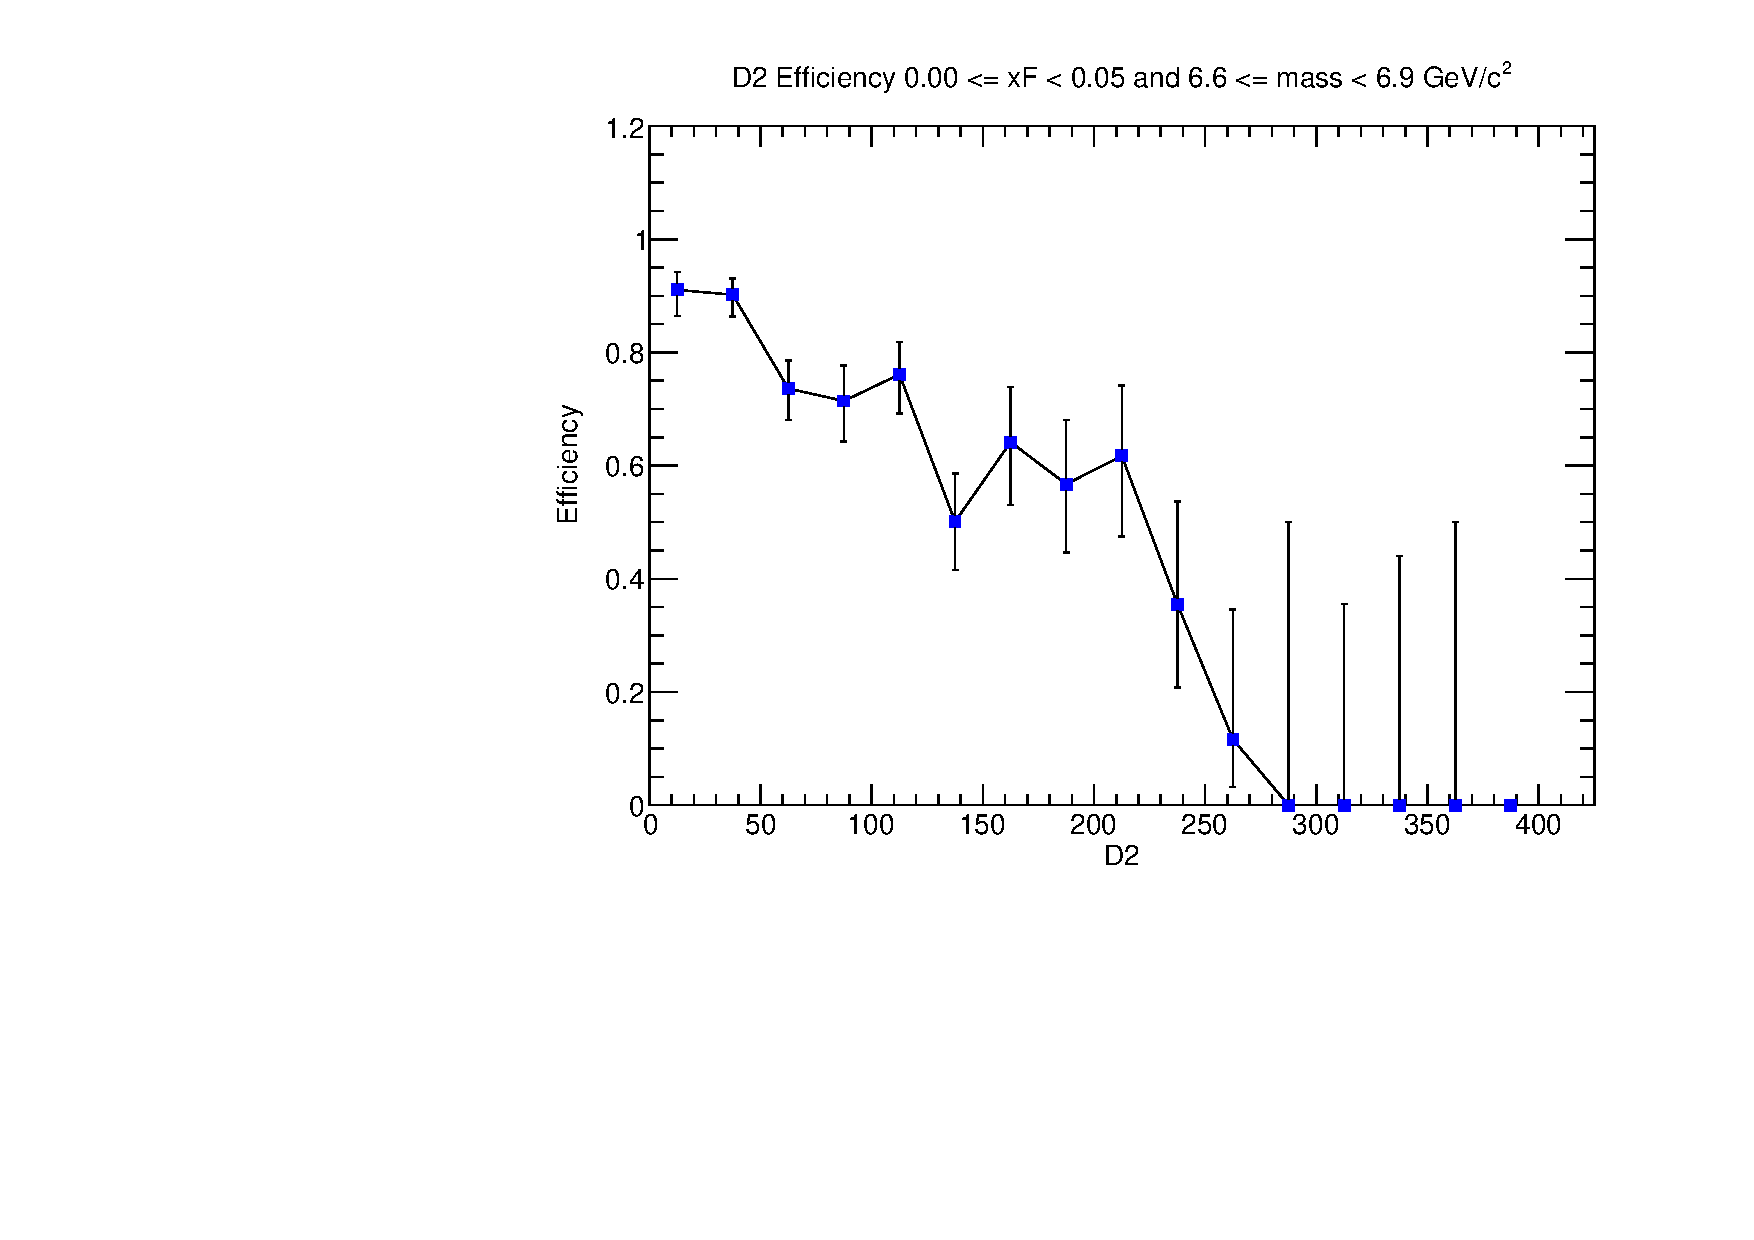
\includegraphics[width=\textwidth]{./kTrackerEfficiencyPlots/D2_Efficiency_xF0_mass8.pdf}
        \caption{$6.6 \leq m < 6.9$ GeV/$c^2$}
        \label{fig:xF0_mass8}
    \end{subfigure}
    \vspace{0.5cm}
    \begin{subfigure}[b]{0.32\textwidth}
        \centering
        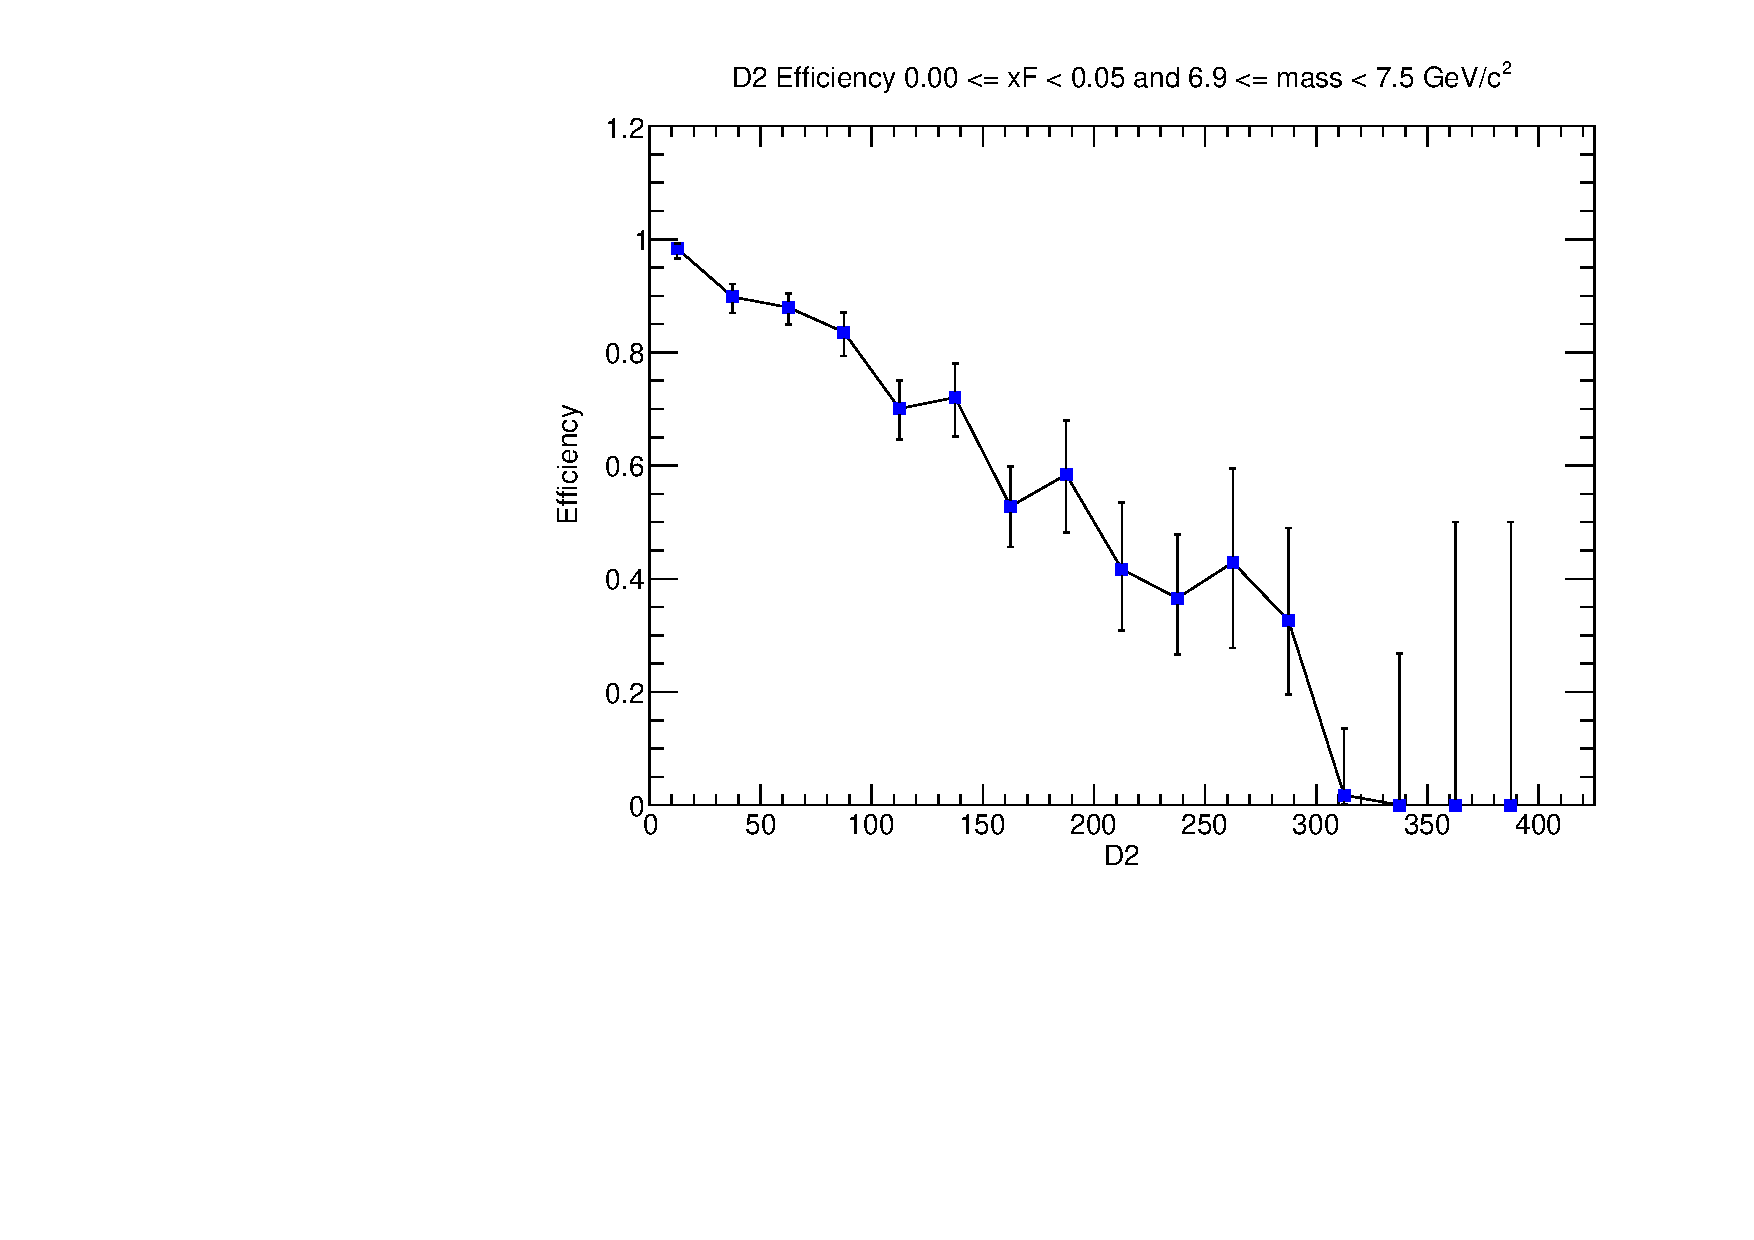
\includegraphics[width=\textwidth]{./kTrackerEfficiencyPlots/D2_Efficiency_xF0_mass9.pdf}
        \caption{$6.9 \leq m < 7.5$ GeV/$c^2$}
        \label{fig:xF0_mass9}
    \end{subfigure}
    \hfill
    \begin{subfigure}[b]{0.32\textwidth}
        \centering
        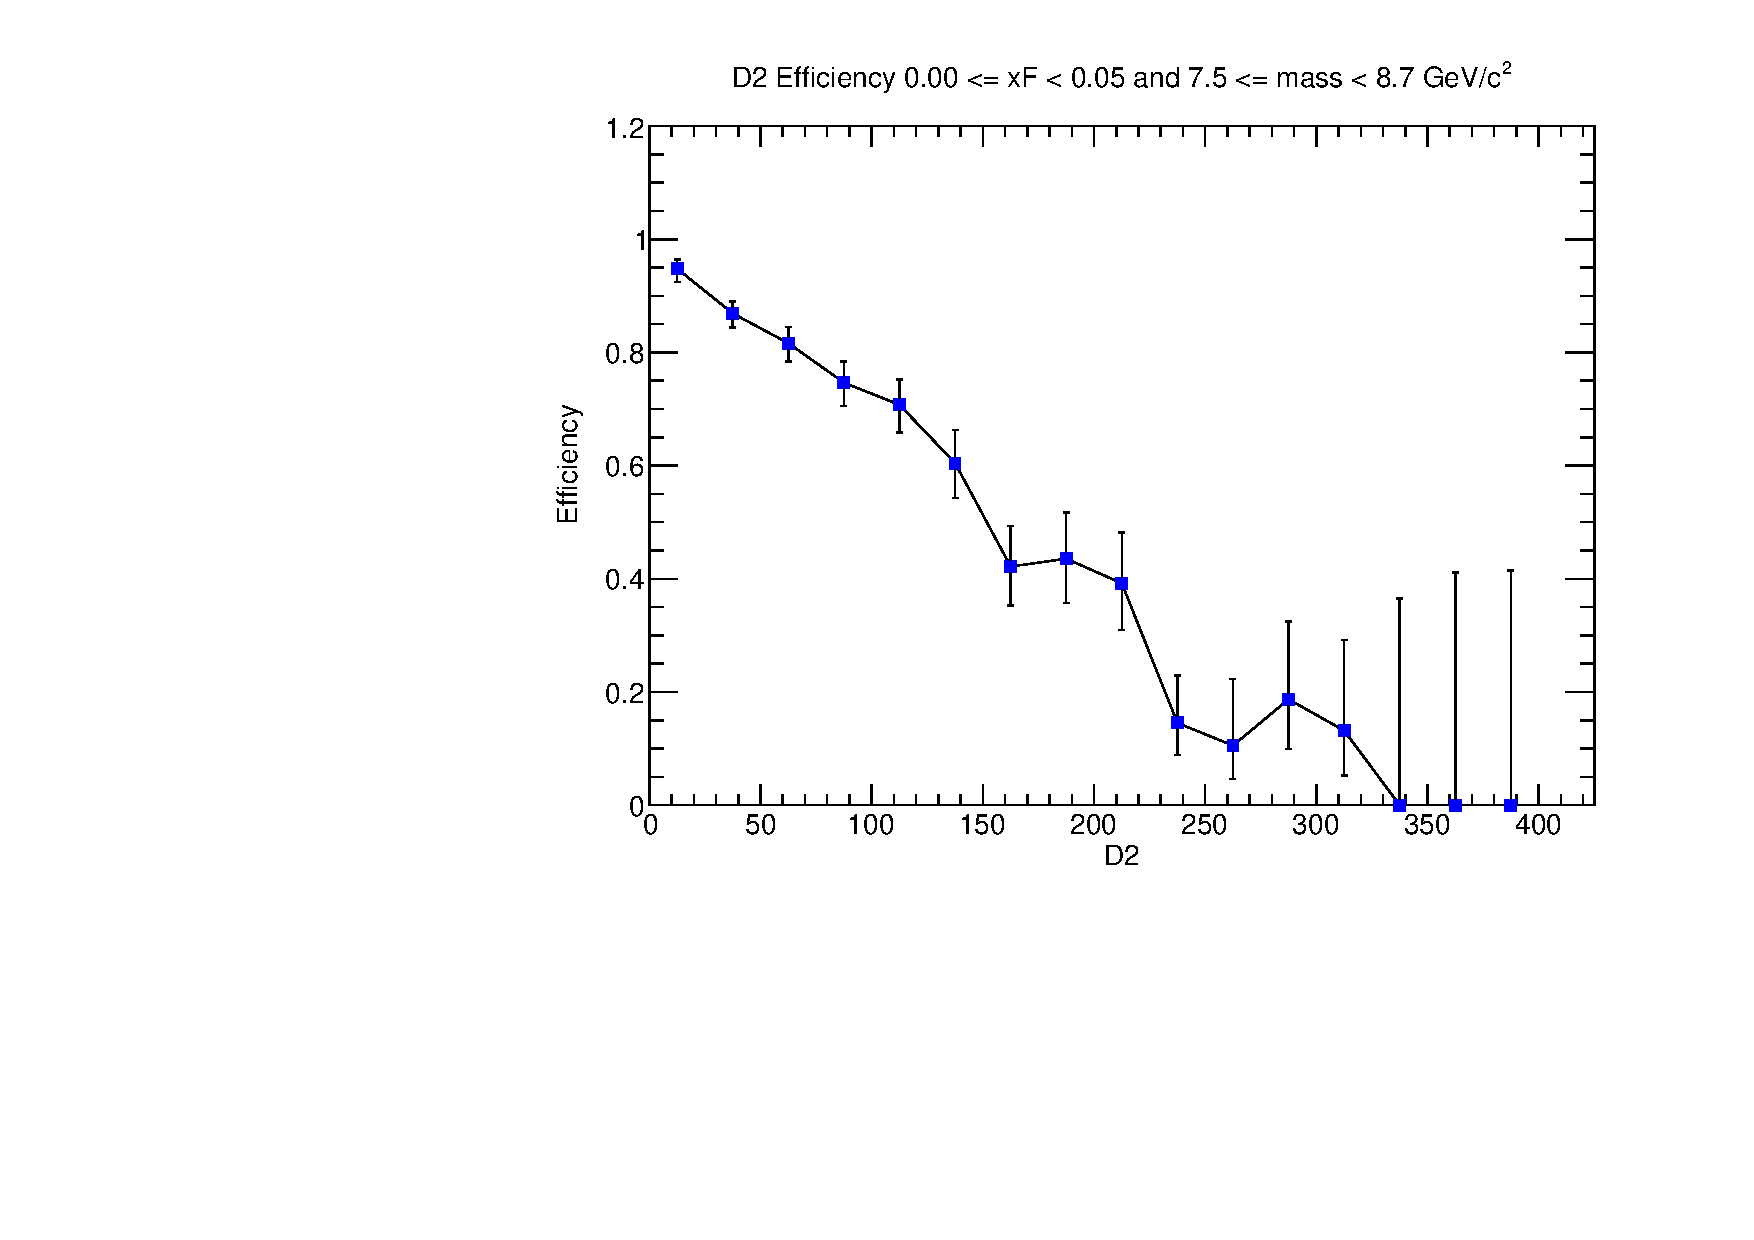
\includegraphics[width=\textwidth]{./kTrackerEfficiencyPlots/D2_Efficiency_xF0_mass10.pdf}
        \caption{$7.5 \leq m < 8.7$ GeV/$c^2$}
        \label{fig:xF0_mass10}
    \end{subfigure}
    \hfill
    \caption{Efficiency plots for the $x_F$ bin $0.00 \leq x_F < 0.05$.}
    \label{fig:xF0}
\end{figure}

\clearpage

\begin{figure}[p]
    \centering
    \begin{subfigure}[b]{0.32\textwidth}
        \centering
        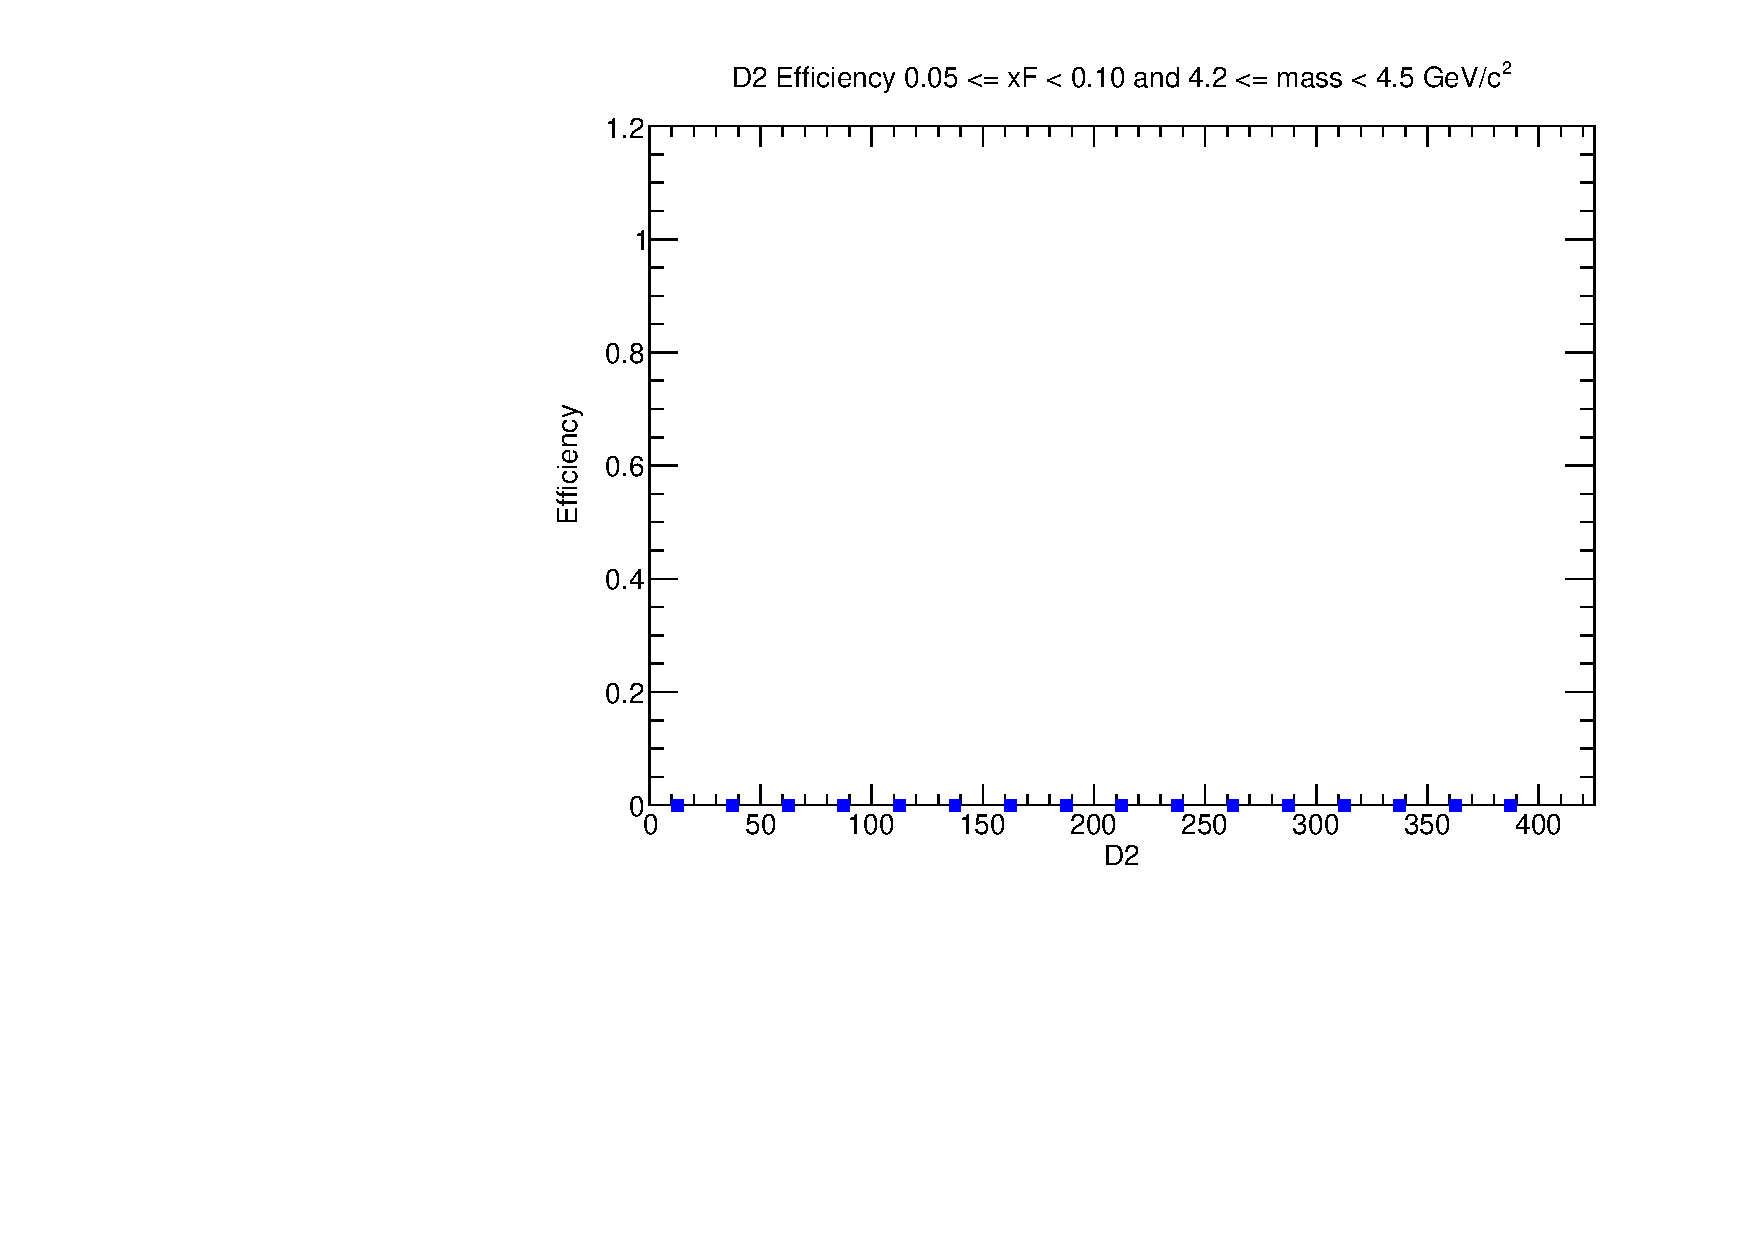
\includegraphics[width=\textwidth]{./kTrackerEfficiencyPlots/D2_Efficiency_xF1_mass0.pdf}
        \caption{$4.2 \leq m < 4.5$ GeV/$c^2$}
        \label{fig:xF1_mass0}
    \end{subfigure}
    \hfill
    \begin{subfigure}[b]{0.32\textwidth}
        \centering
        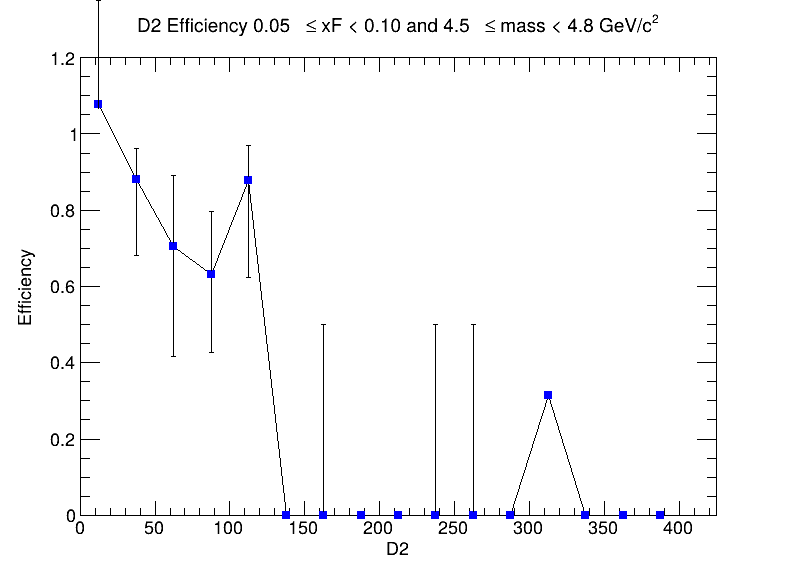
\includegraphics[width=\textwidth]{./kTrackerEfficiencyPlots/D2_Efficiency_xF1_mass1.png}
        \caption{$4.5 \leq m < 4.8$ GeV/$c^2$}
        \label{fig:xF1_mass1}
    \end{subfigure}
    \hfill
    \begin{subfigure}[b]{0.32\textwidth}
        \centering
        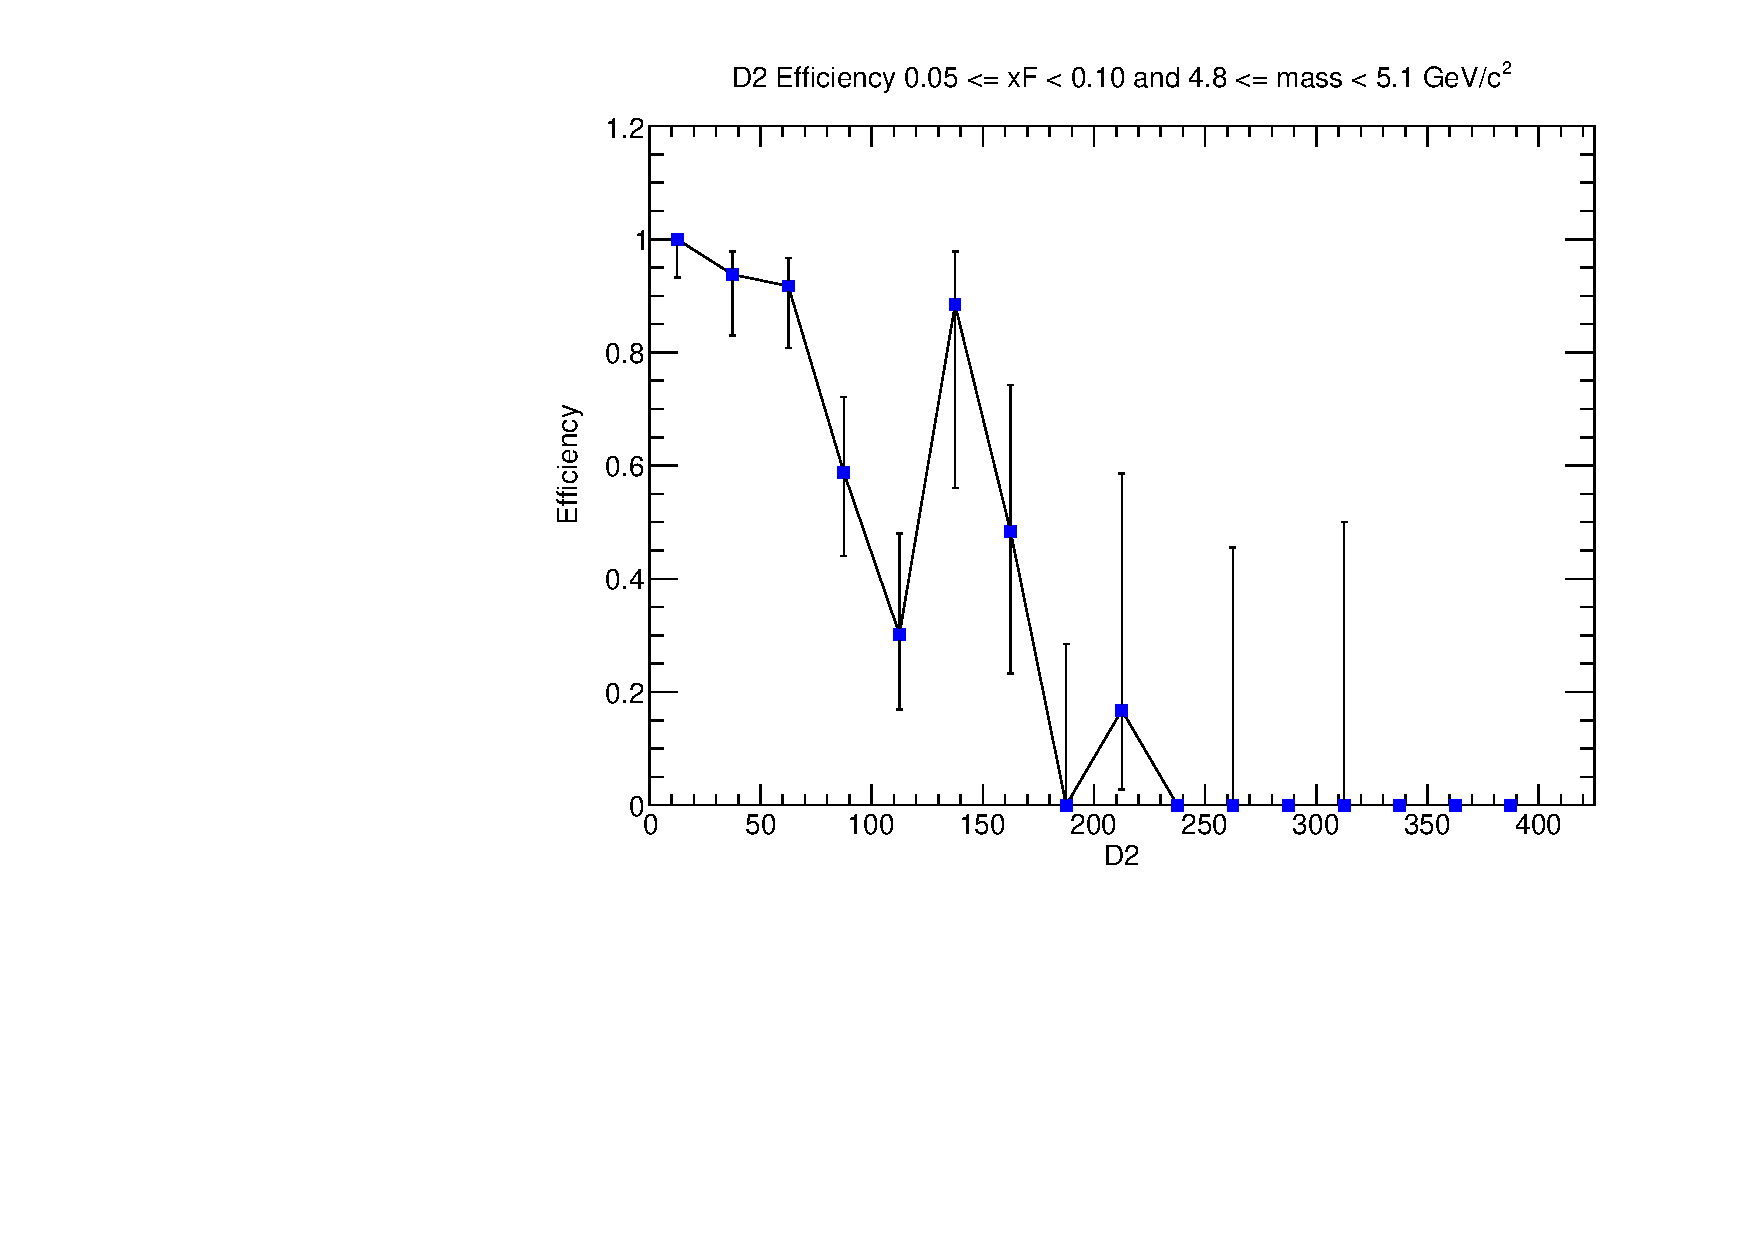
\includegraphics[width=\textwidth]{./kTrackerEfficiencyPlots/D2_Efficiency_xF1_mass2.pdf}
        \caption{$4.8 \leq m < 5.1$ GeV/$c^2$}
        \label{fig:xF1_mass2}
    \end{subfigure}
    \vspace{0.5cm}
    \begin{subfigure}[b]{0.32\textwidth}
        \centering
        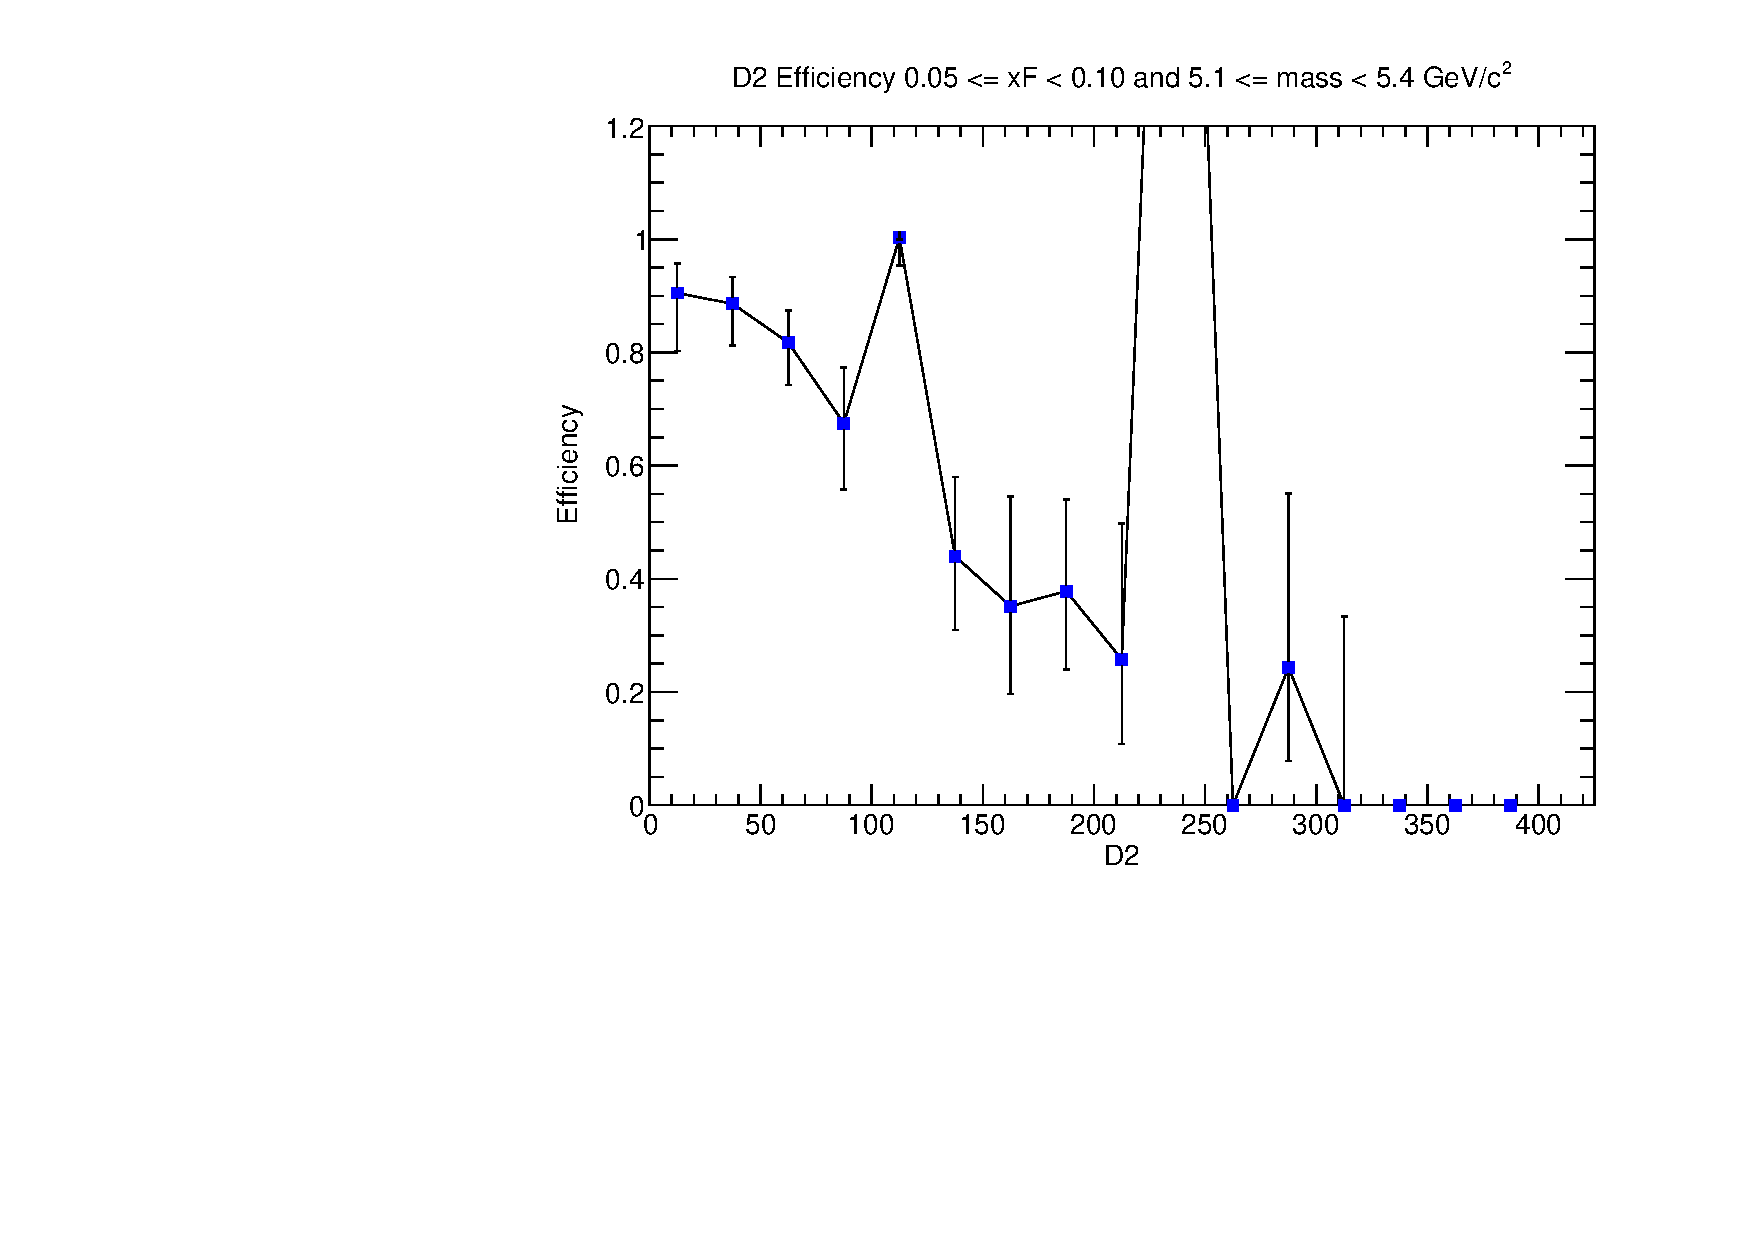
\includegraphics[width=\textwidth]{./kTrackerEfficiencyPlots/D2_Efficiency_xF1_mass3.pdf}
        \caption{$5.1 \leq m < 5.4$ GeV/$c^2$}
        \label{fig:xF1_mass3}
    \end{subfigure}
    \hfill
    \begin{subfigure}[b]{0.32\textwidth}
        \centering
        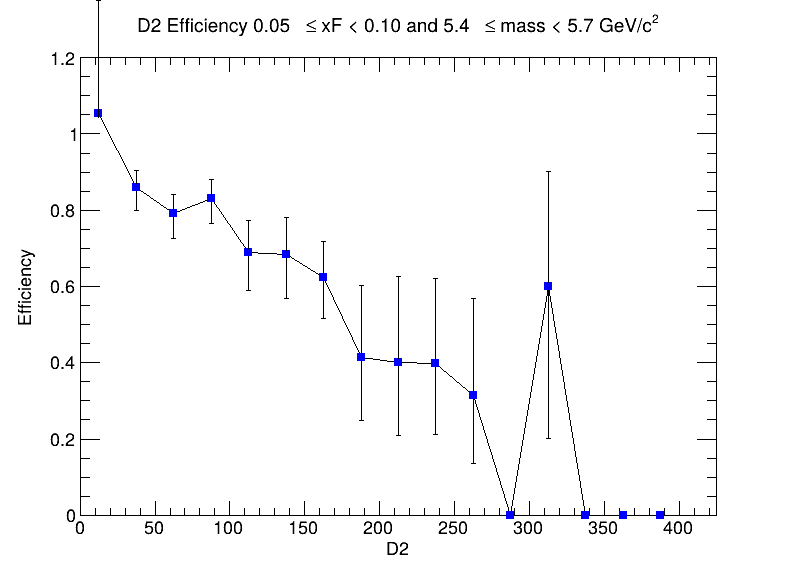
\includegraphics[width=\textwidth]{./kTrackerEfficiencyPlots/D2_Efficiency_xF1_mass4.png}
        \caption{$5.4 \leq m < 5.7$ GeV/$c^2$}
        \label{fig:xF1_mass4}
    \end{subfigure}
    \hfill
    \begin{subfigure}[b]{0.32\textwidth}
        \centering
        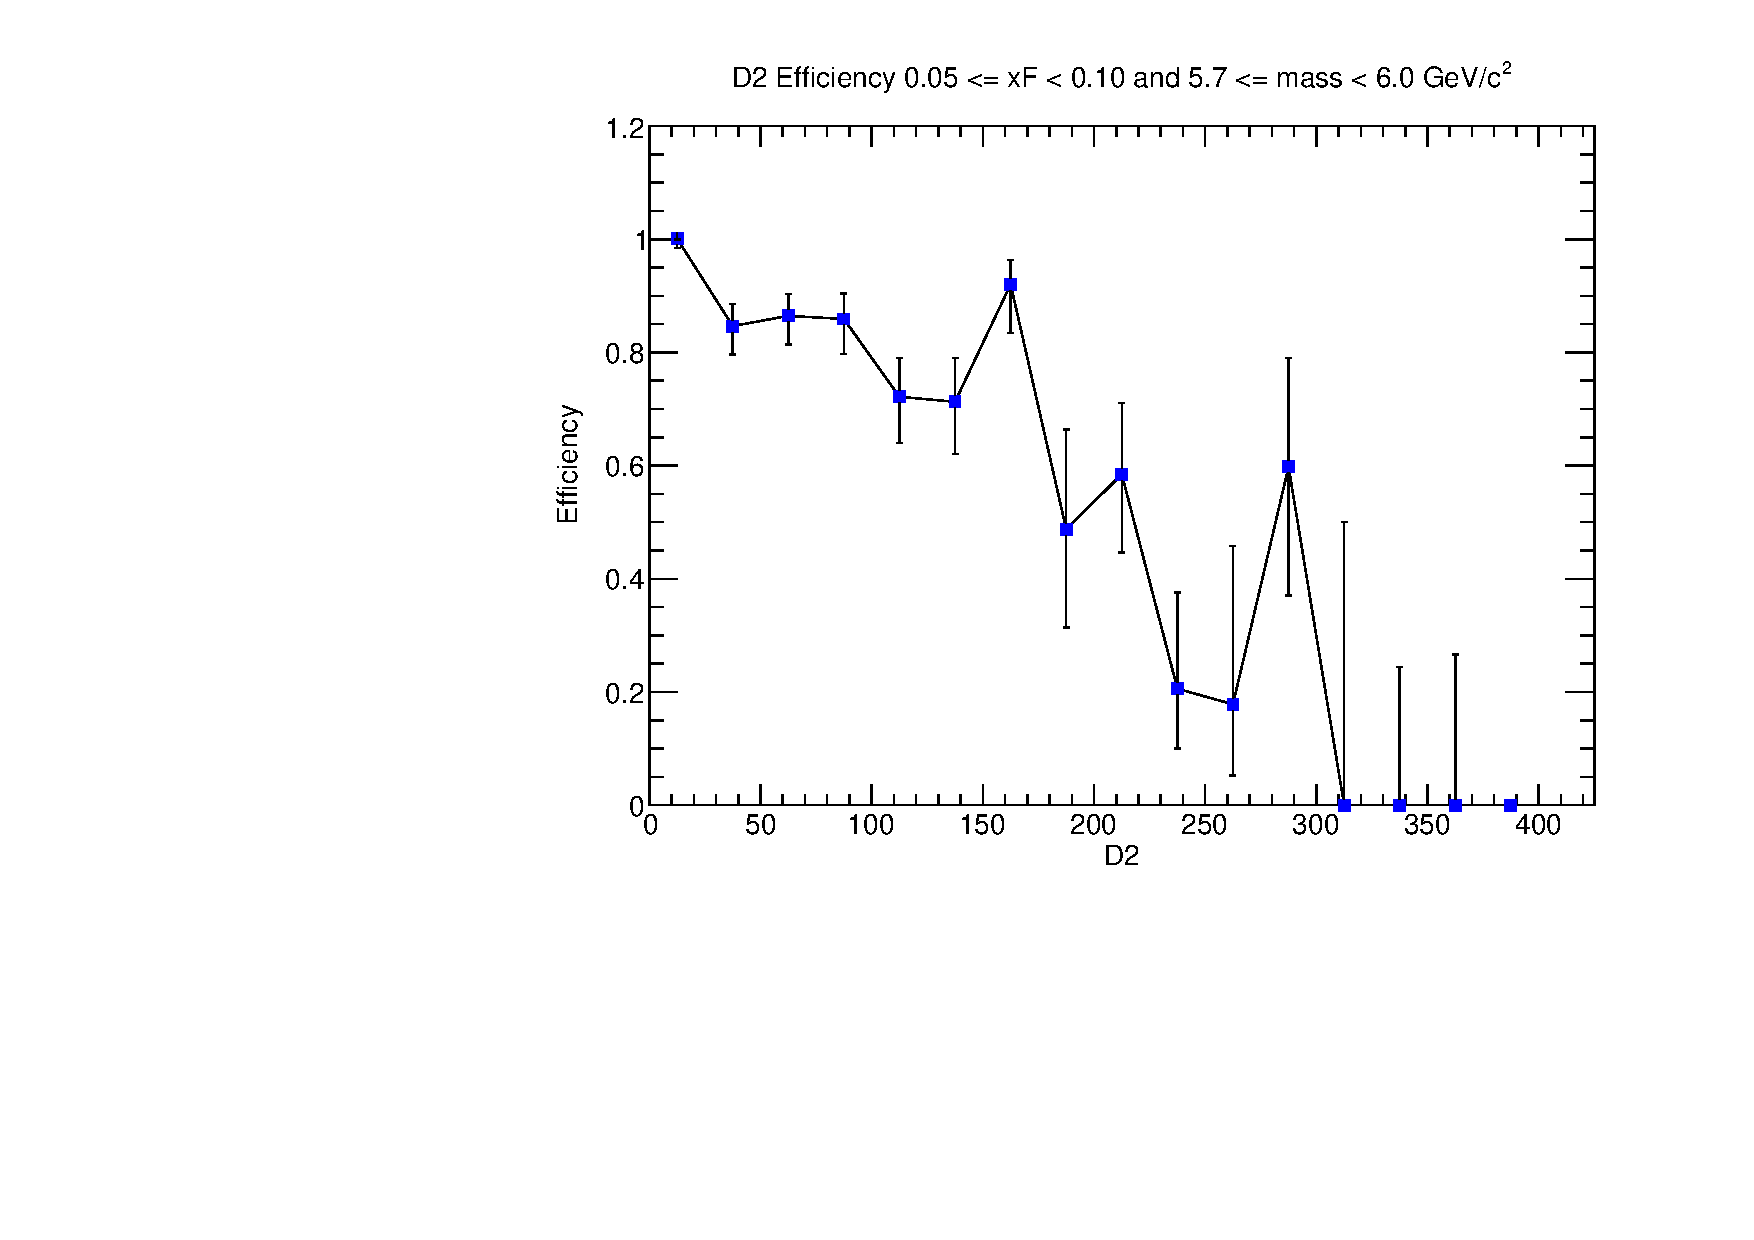
\includegraphics[width=\textwidth]{./kTrackerEfficiencyPlots/D2_Efficiency_xF1_mass5.pdf}
        \caption{$5.7 \leq m < 6.0$ GeV/$c^2$}
        \label{fig:xF1_mass5}
    \end{subfigure}
    \vspace{0.5cm}
    \begin{subfigure}[b]{0.32\textwidth}
        \centering
        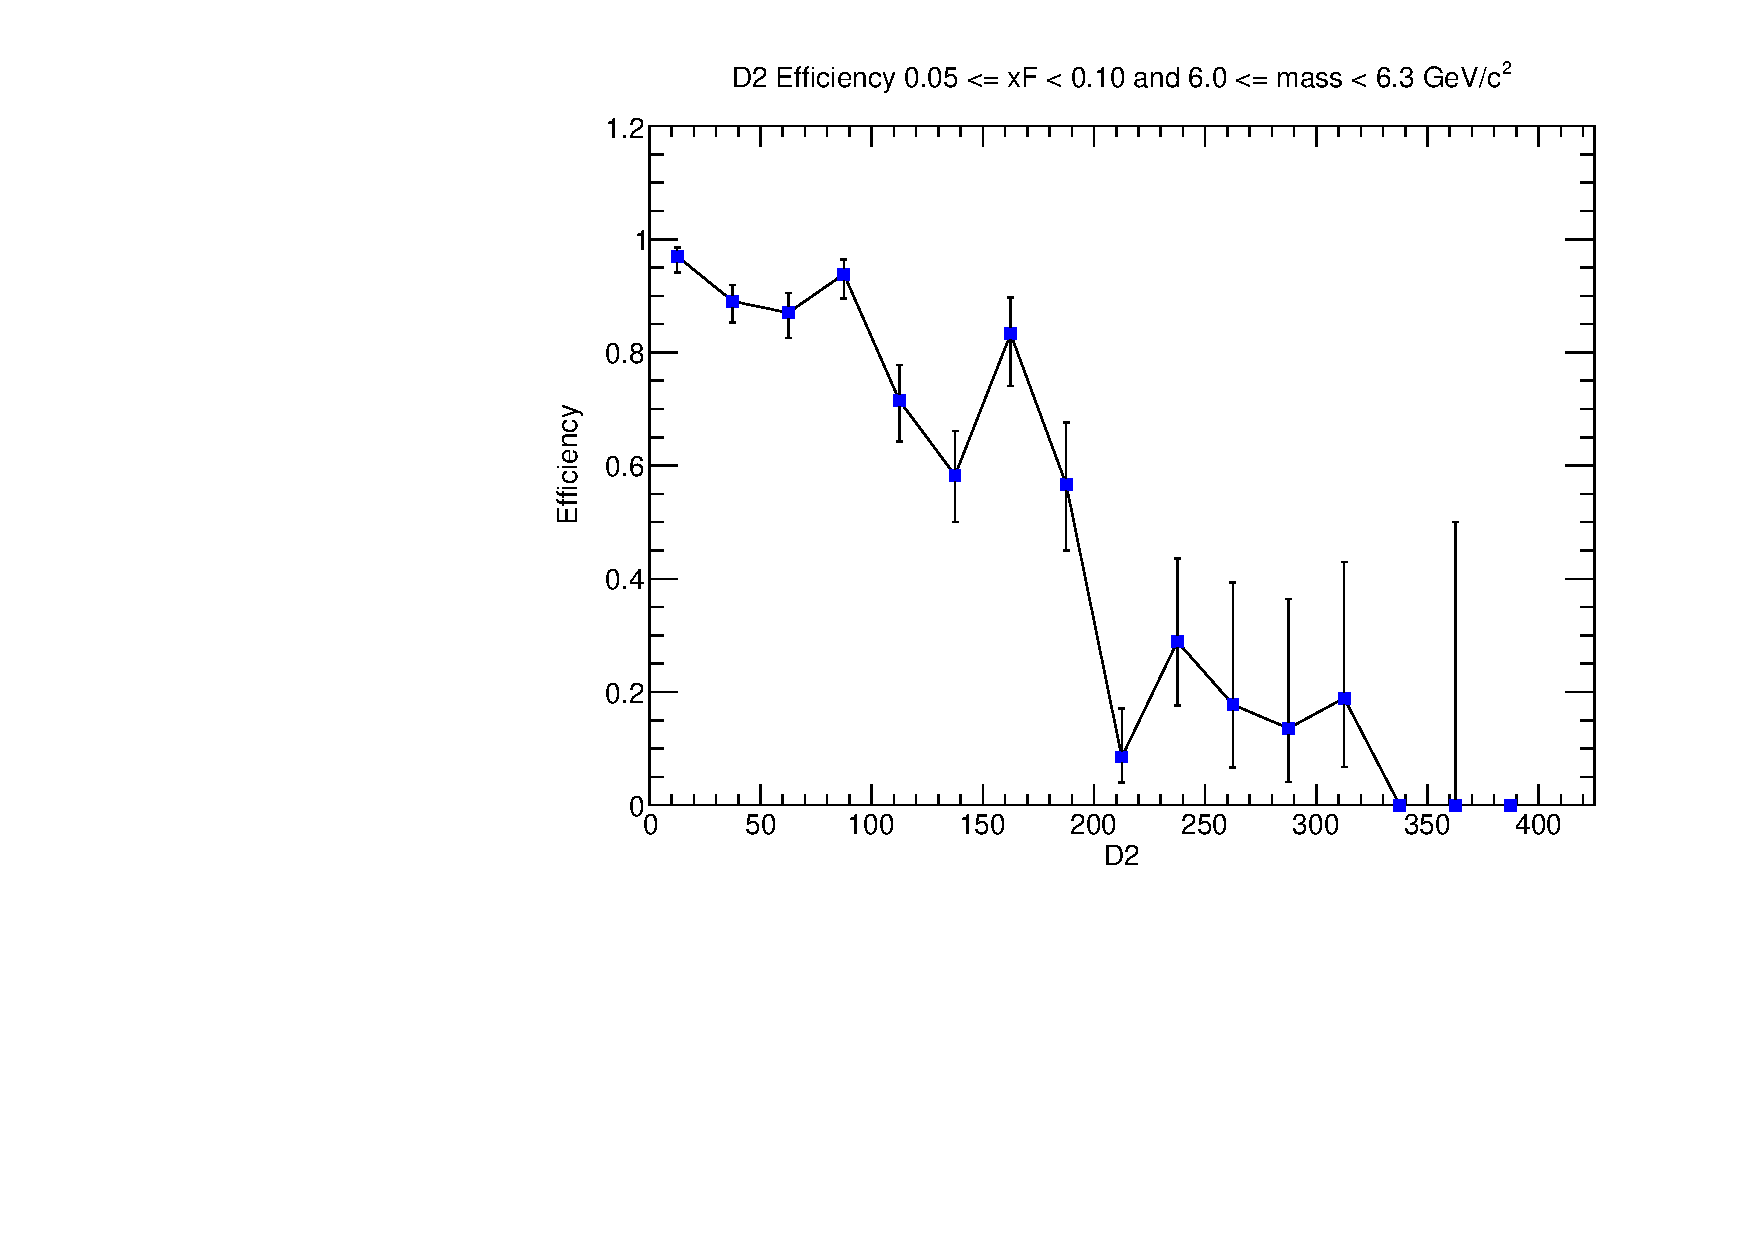
\includegraphics[width=\textwidth]{./kTrackerEfficiencyPlots/D2_Efficiency_xF1_mass6.pdf}
        \caption{$6.0 \leq m < 6.3$ GeV/$c^2$}
        \label{fig:xF1_mass6}
    \end{subfigure}
    \hfill
    \begin{subfigure}[b]{0.32\textwidth}
        \centering
        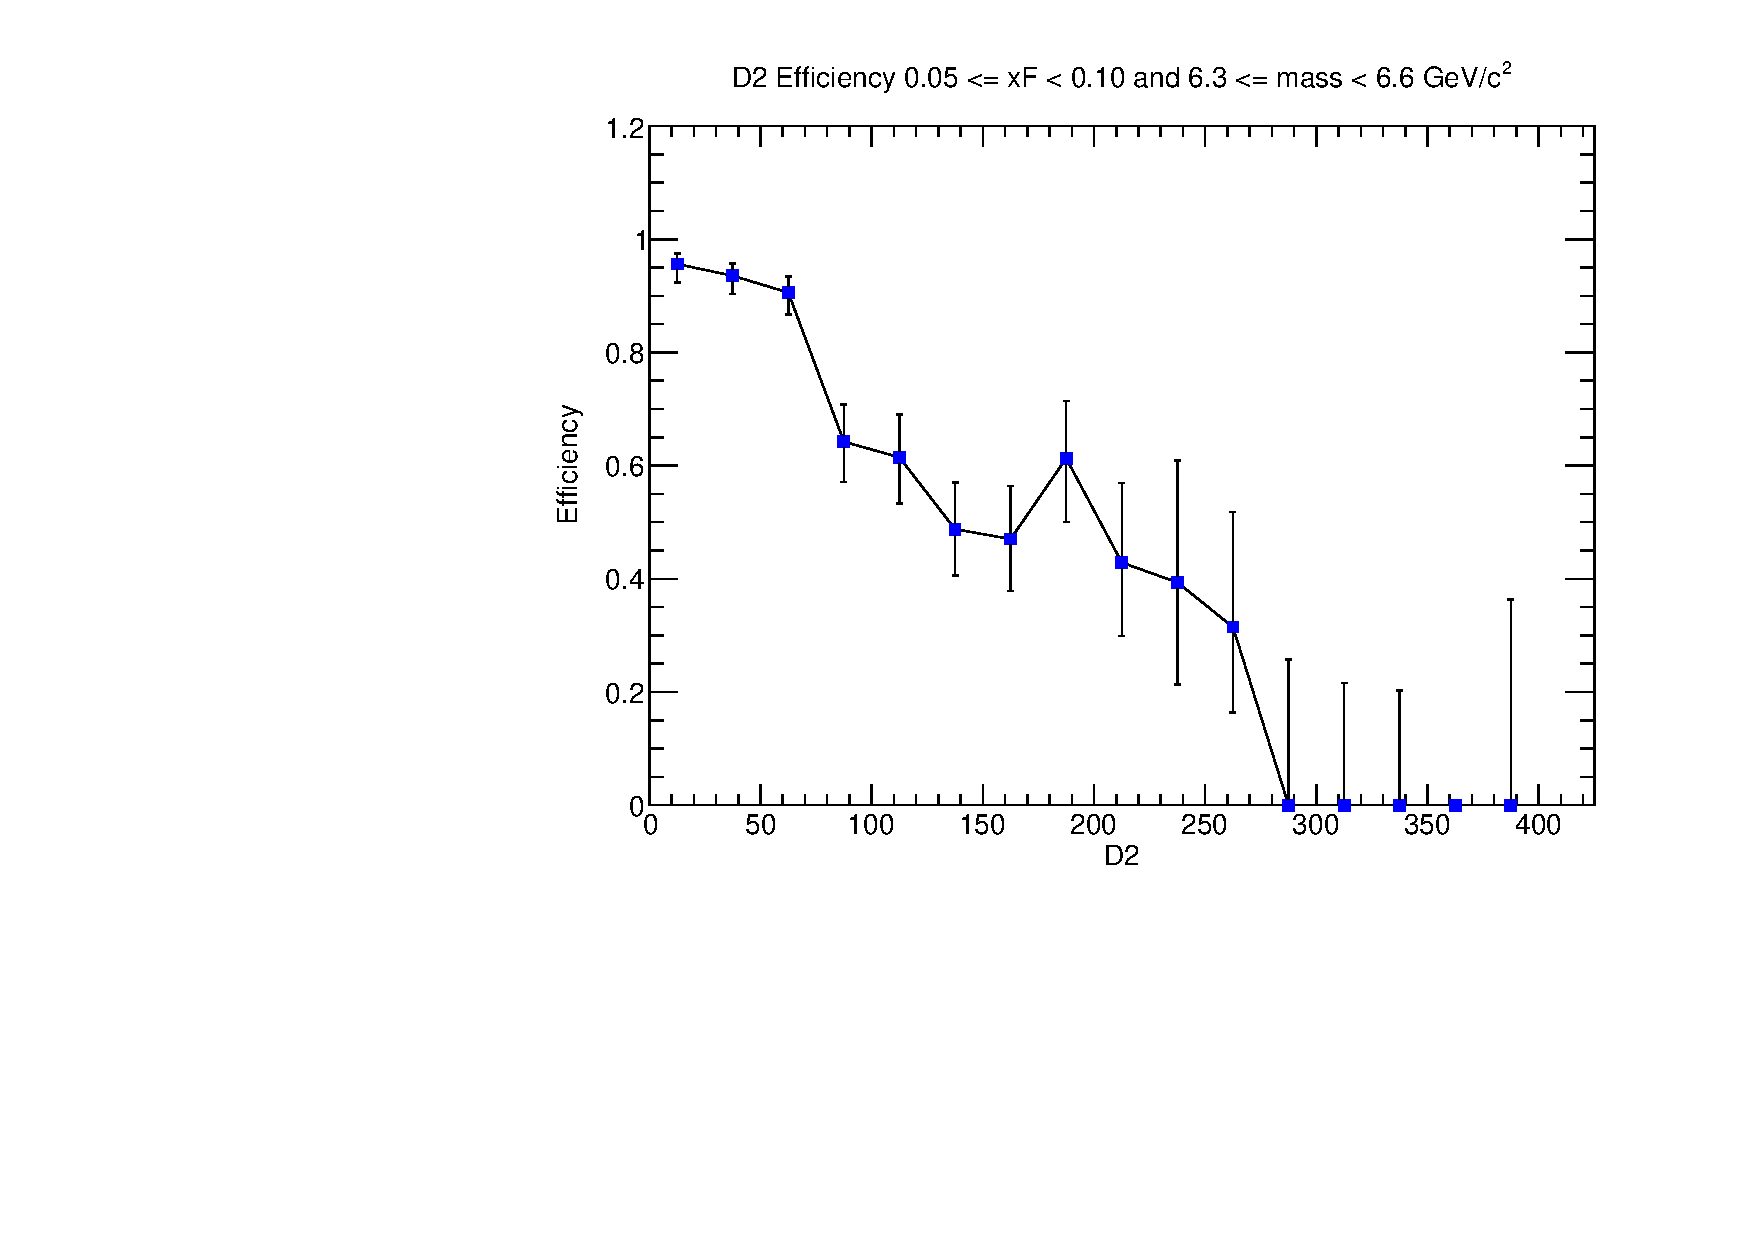
\includegraphics[width=\textwidth]{./kTrackerEfficiencyPlots/D2_Efficiency_xF1_mass7.pdf}
        \caption{$6.3 \leq m < 6.6$ GeV/$c^2$}
        \label{fig:xF1_mass7}
    \end{subfigure}
    \hfill
    \begin{subfigure}[b]{0.32\textwidth}
        \centering
        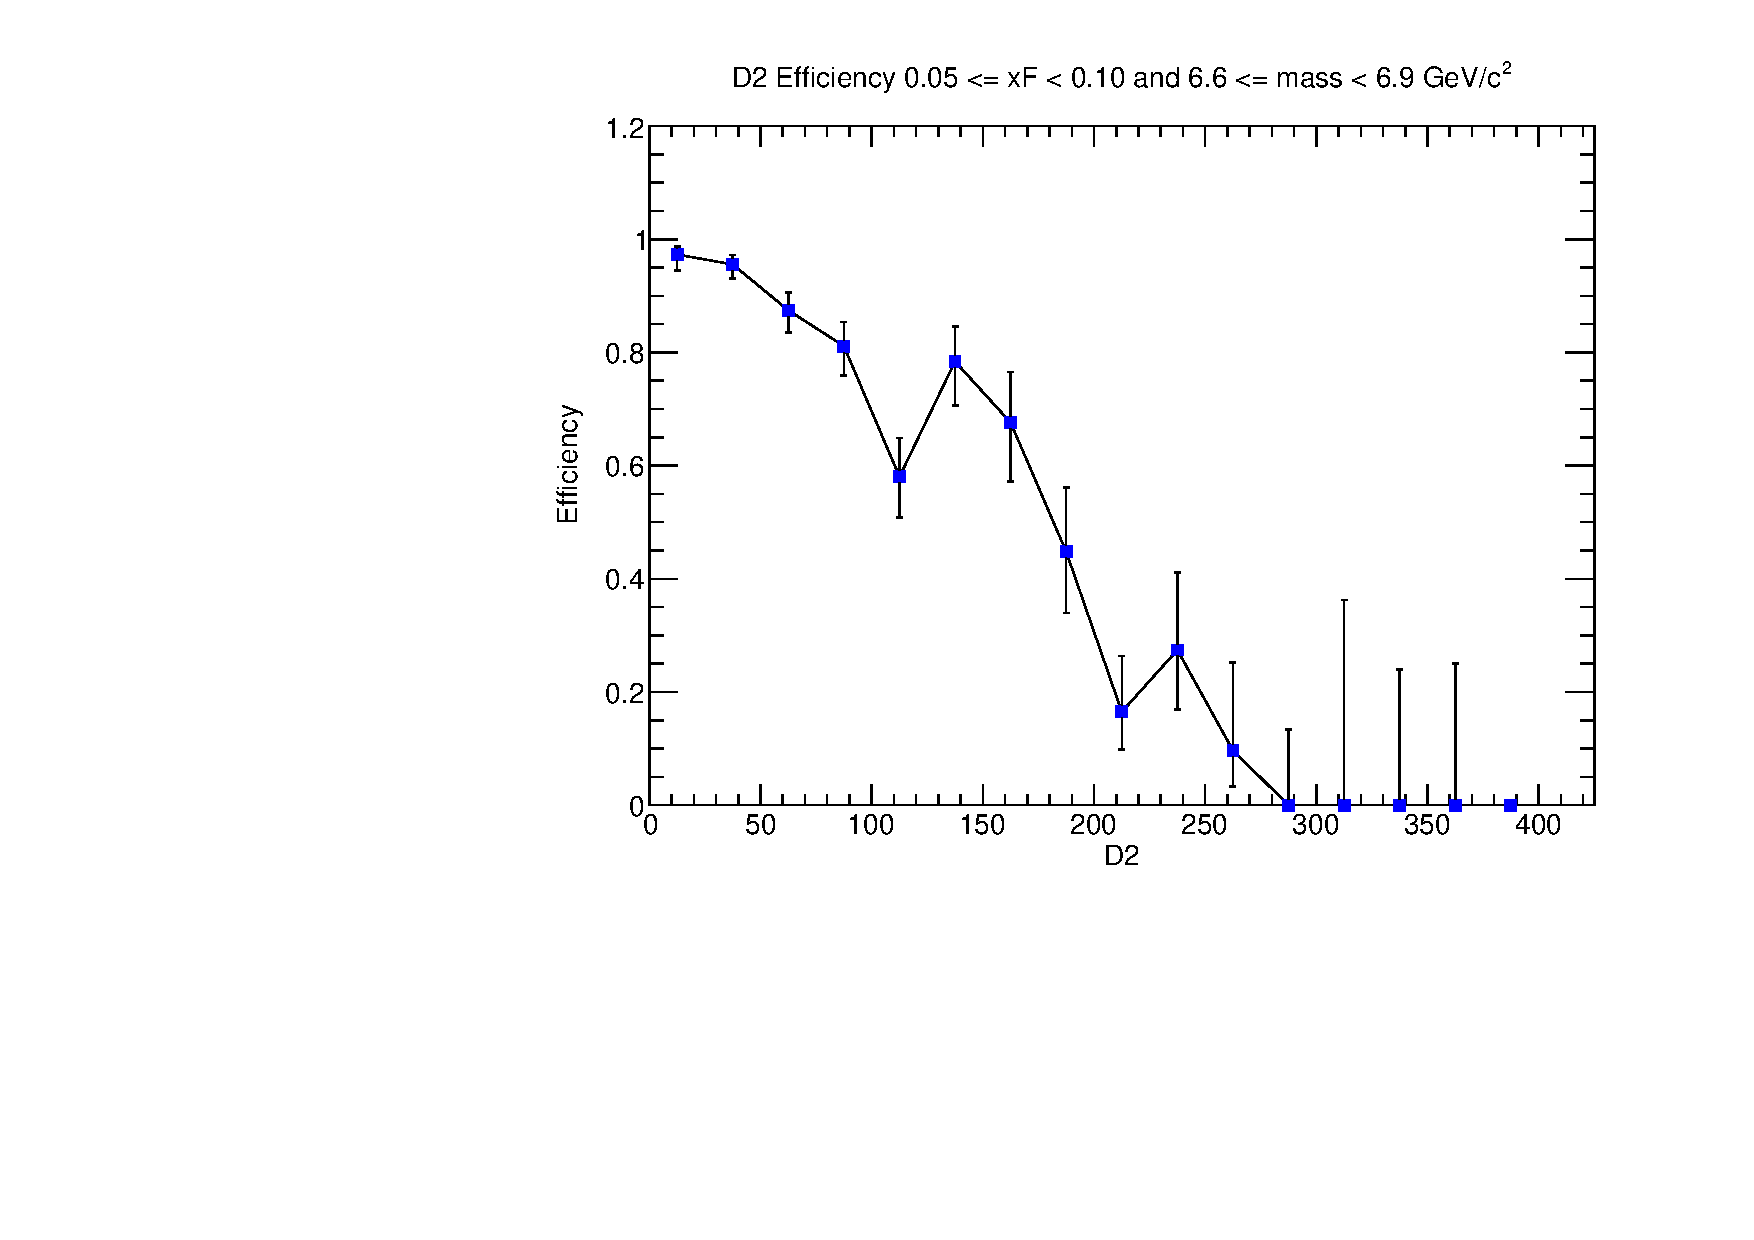
\includegraphics[width=\textwidth]{./kTrackerEfficiencyPlots/D2_Efficiency_xF1_mass8.pdf}
        \caption{$6.6 \leq m < 6.9$ GeV/$c^2$}
        \label{fig:xF1_mass8}
    \end{subfigure}
    \vspace{0.5cm}
    \begin{subfigure}[b]{0.32\textwidth}
        \centering
        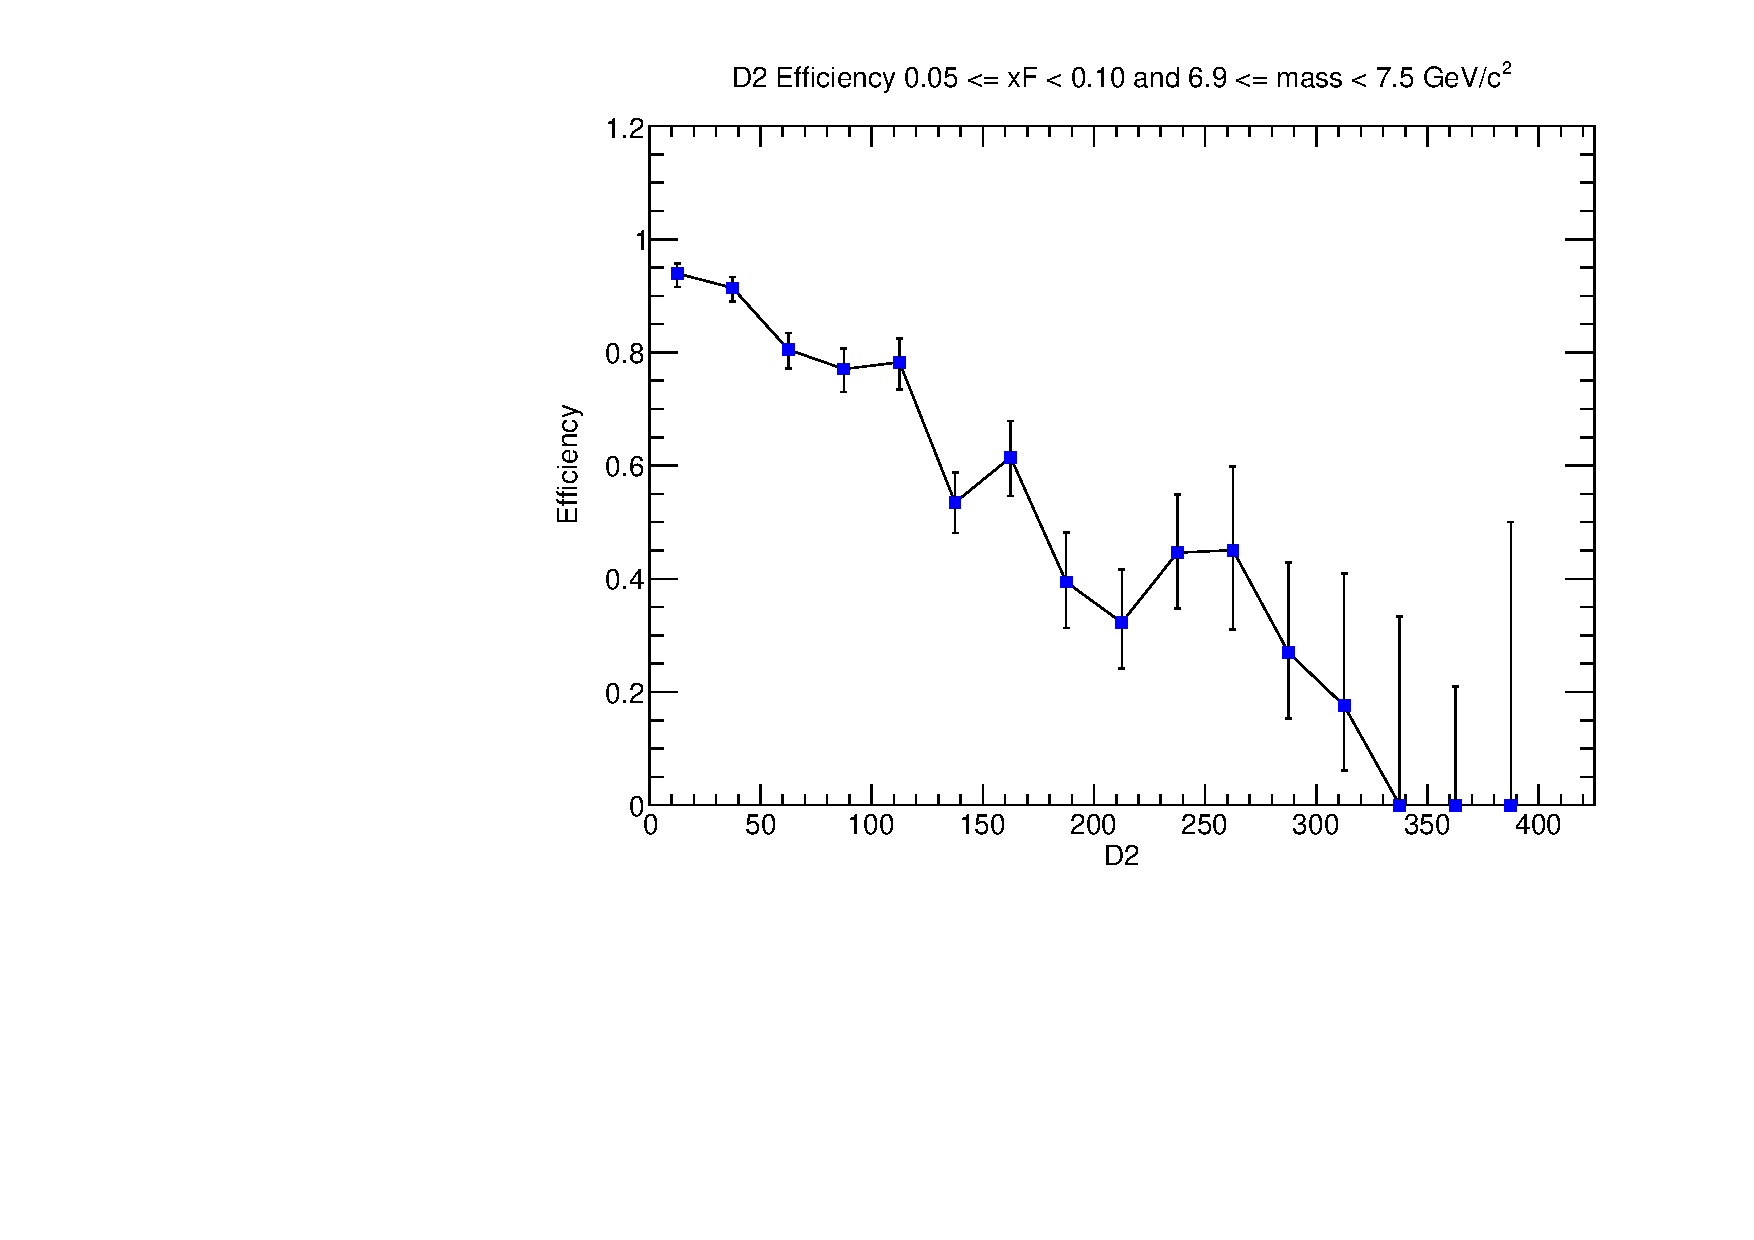
\includegraphics[width=\textwidth]{./kTrackerEfficiencyPlots/D2_Efficiency_xF1_mass9.pdf}
        \caption{$6.9 \leq m < 7.5$ GeV/$c^2$}
        \label{fig:xF1_mass9}
    \end{subfigure}
    \hfill
    \begin{subfigure}[b]{0.32\textwidth}
        \centering
        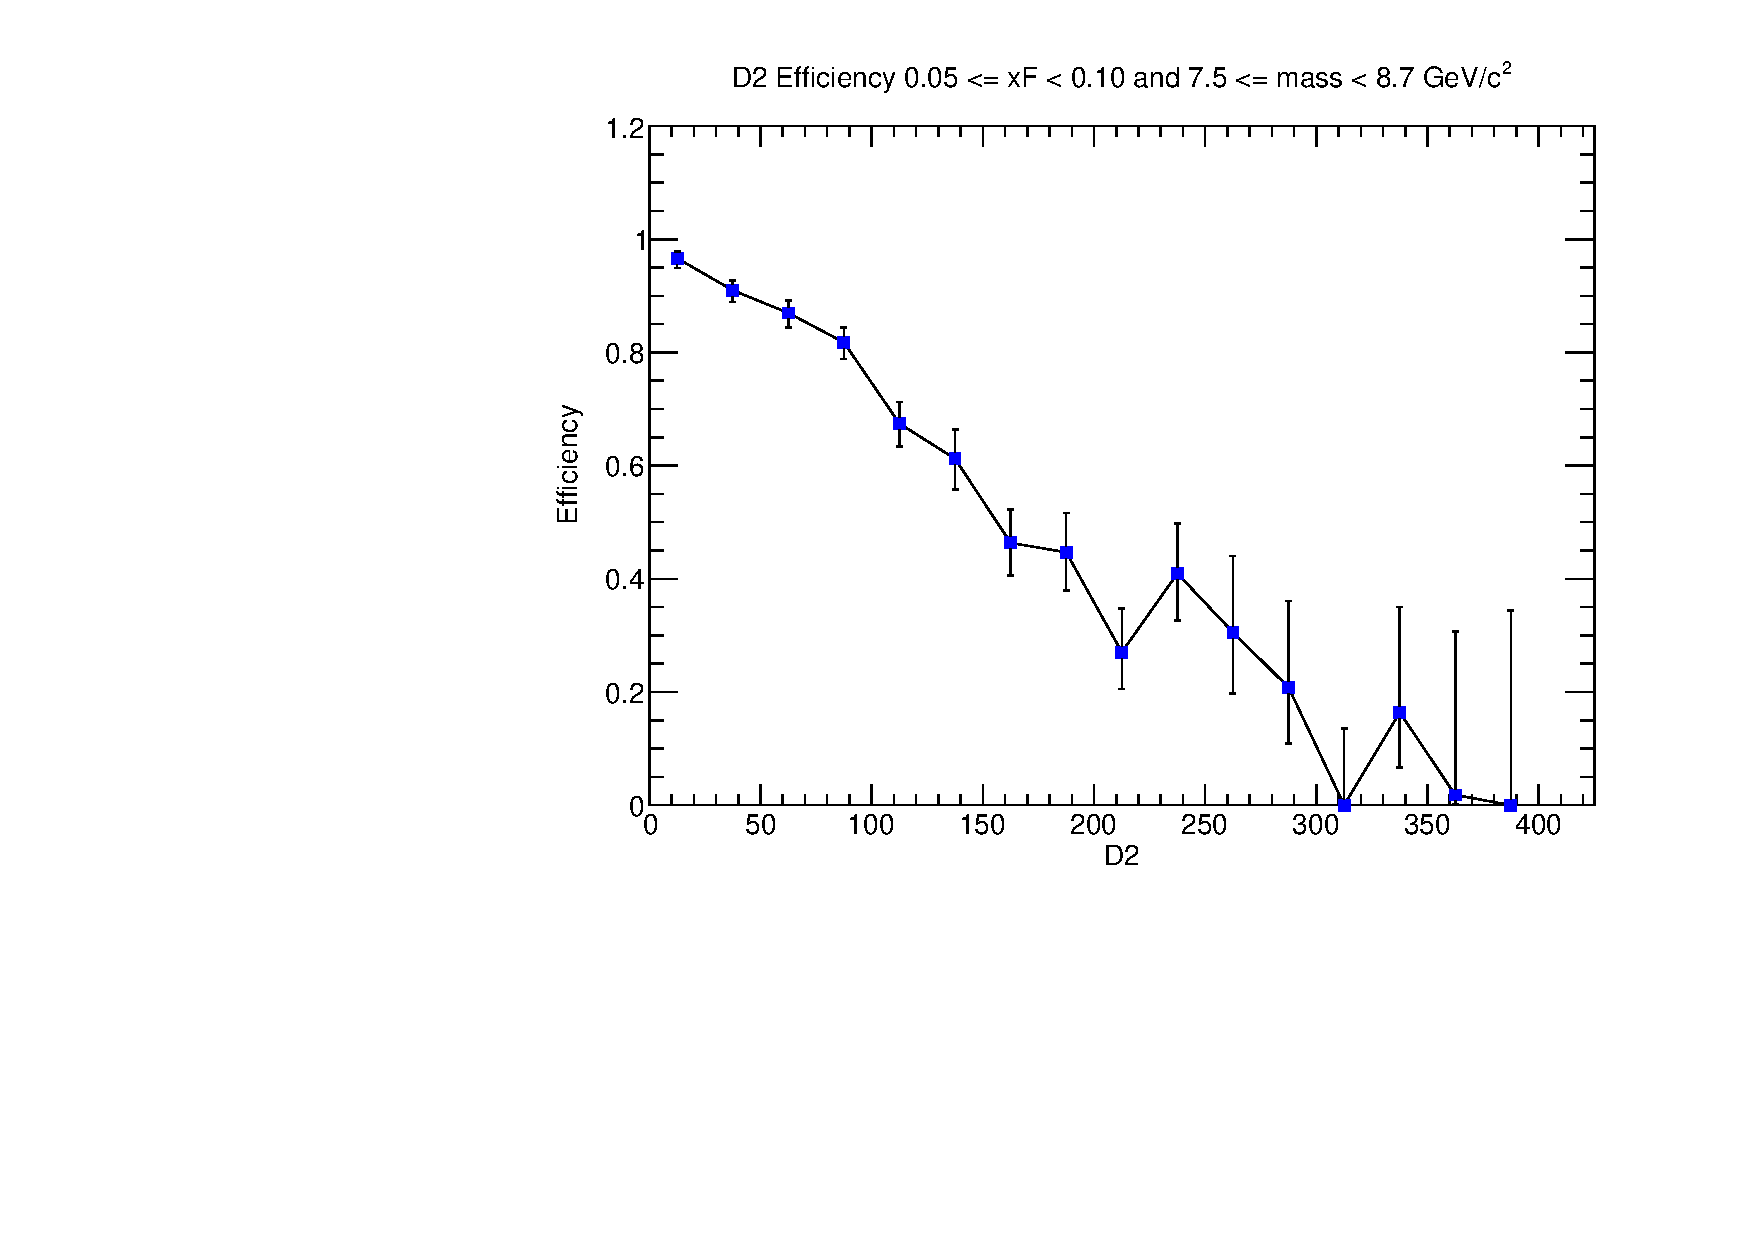
\includegraphics[width=\textwidth]{./kTrackerEfficiencyPlots/D2_Efficiency_xF1_mass10.pdf}
        \caption{$7.5 \leq m < 8.7$ GeV/$c^2$}
        \label{fig:xF1_mass10}
    \end{subfigure}
    \hfill
    \caption{Efficiency plots for the $x_F$ bin $0.05 \leq x_F < 0.10$.}
    \label{fig:xF1}
\end{figure}

\clearpage

\begin{figure}[p]
    \centering
    \begin{subfigure}[b]{0.32\textwidth}
        \centering
        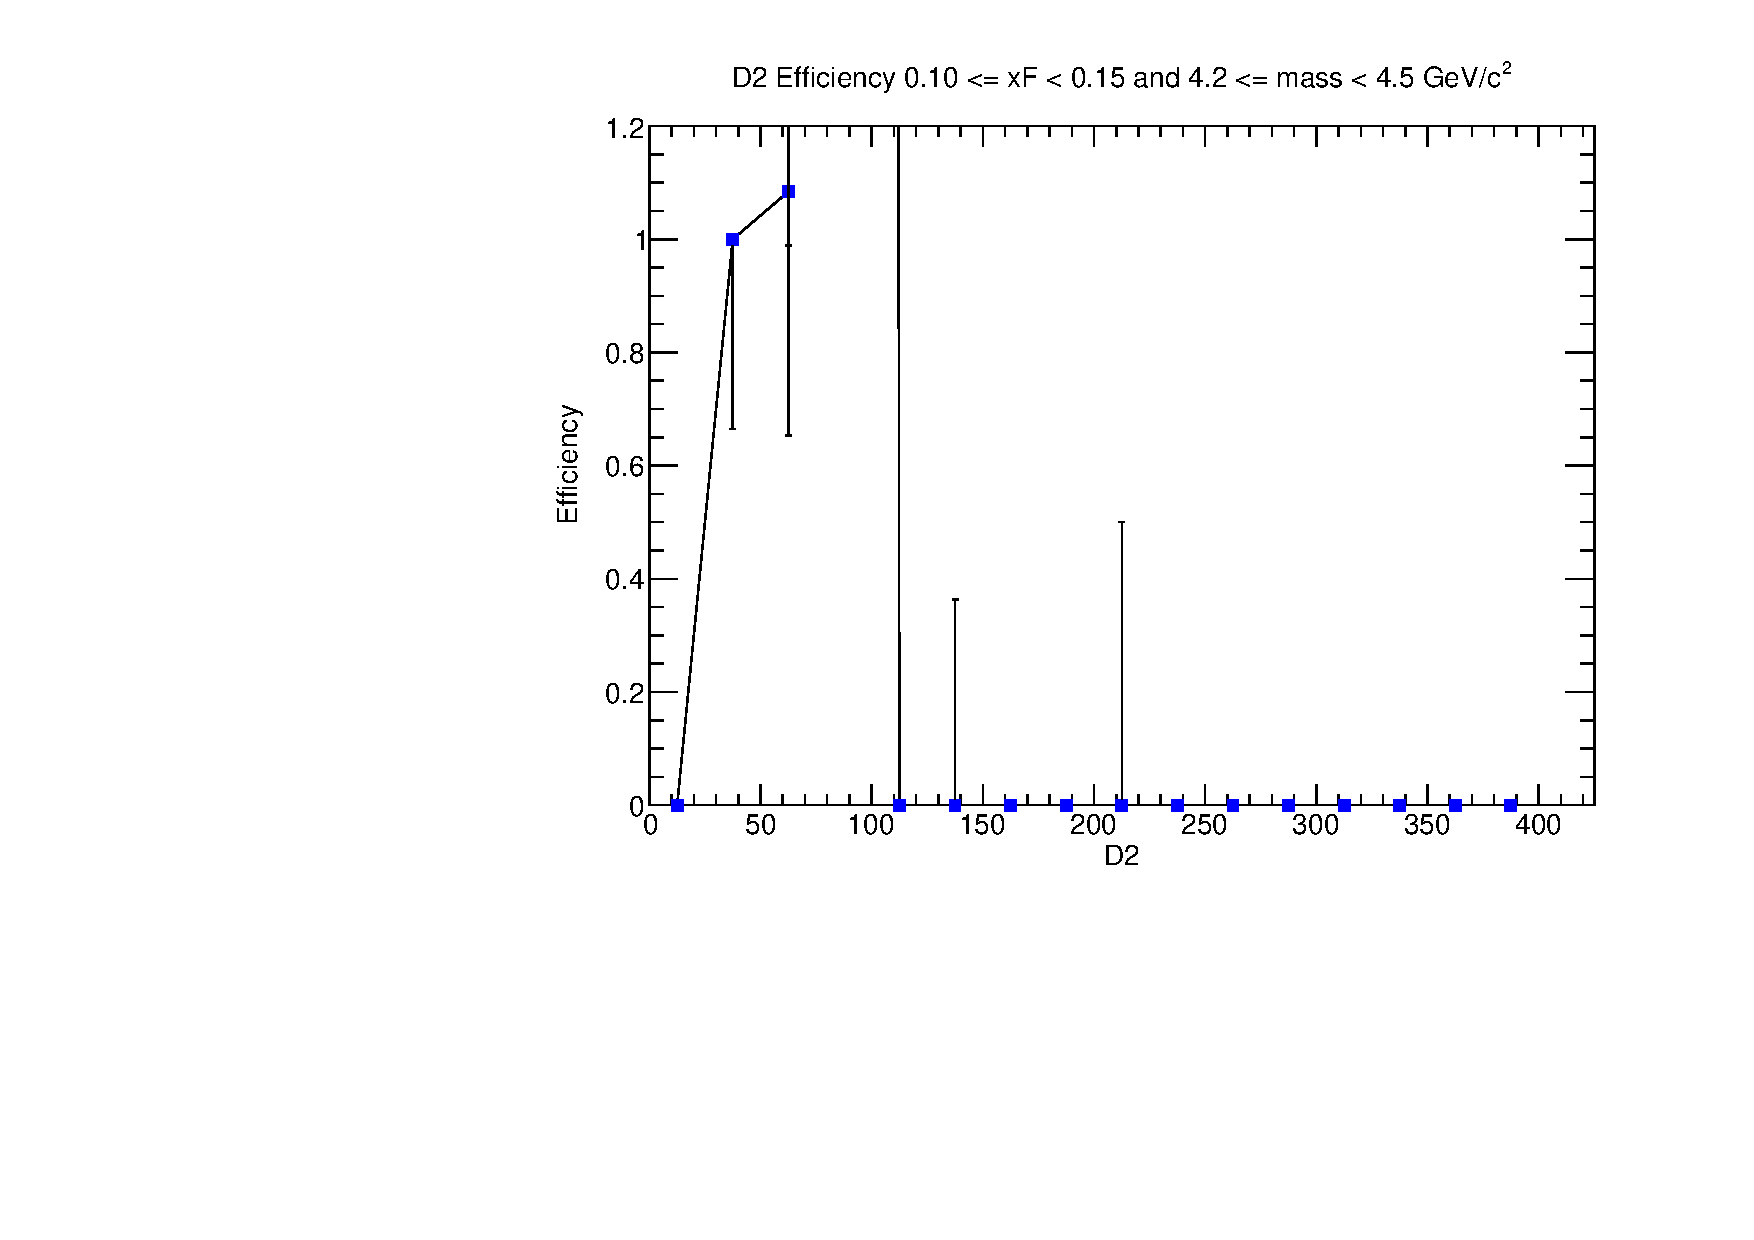
\includegraphics[width=\textwidth]{./kTrackerEfficiencyPlots/D2_Efficiency_xF2_mass0.pdf}
        \caption{$4.2 \leq m < 4.5$ GeV/$c^2$}
        \label{fig:xF2_mass0}
    \end{subfigure}
    \hfill
    \begin{subfigure}[b]{0.32\textwidth}
        \centering
        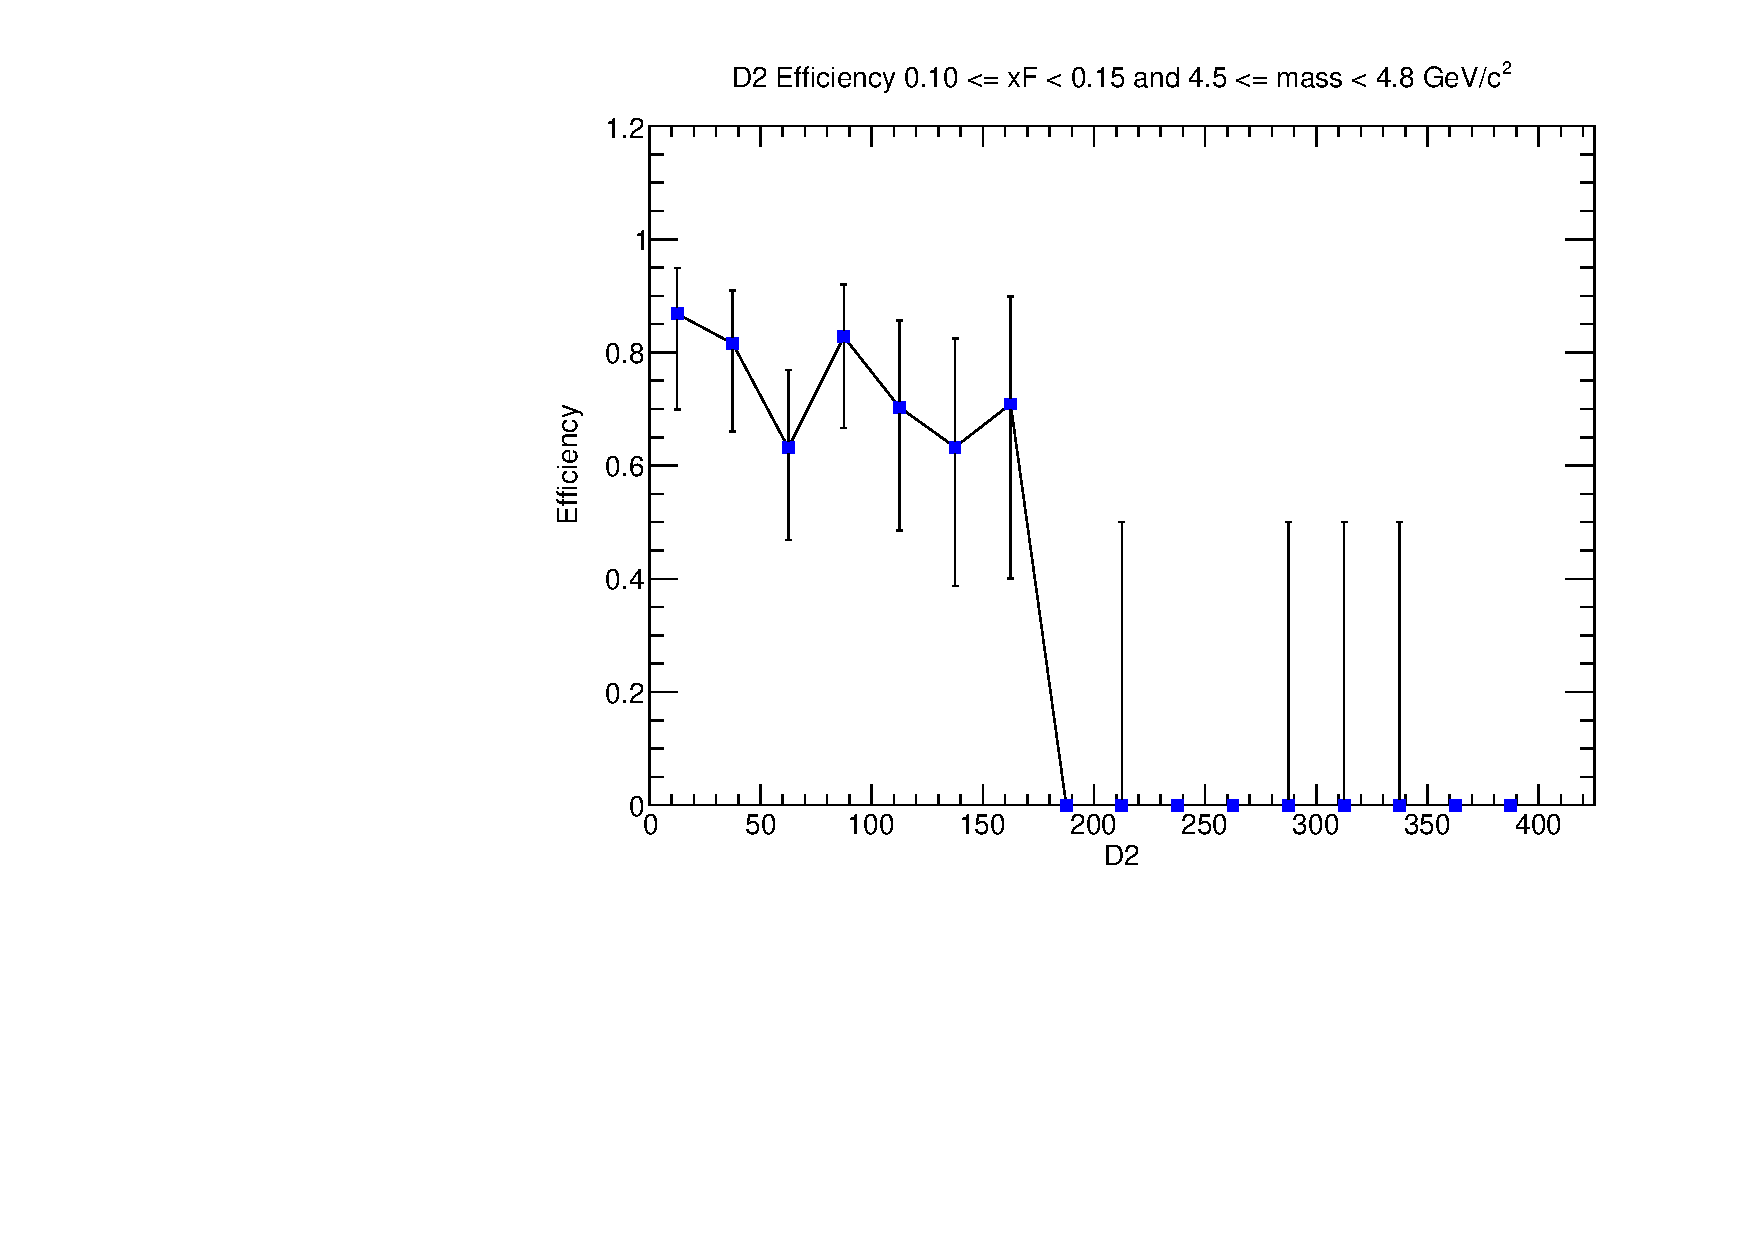
\includegraphics[width=\textwidth]{./kTrackerEfficiencyPlots/D2_Efficiency_xF2_mass1.pdf}
        \caption{$4.5 \leq m < 4.8$ GeV/$c^2$}
        \label{fig:xF2_mass1}
    \end{subfigure}
    \hfill
    \begin{subfigure}[b]{0.32\textwidth}
        \centering
        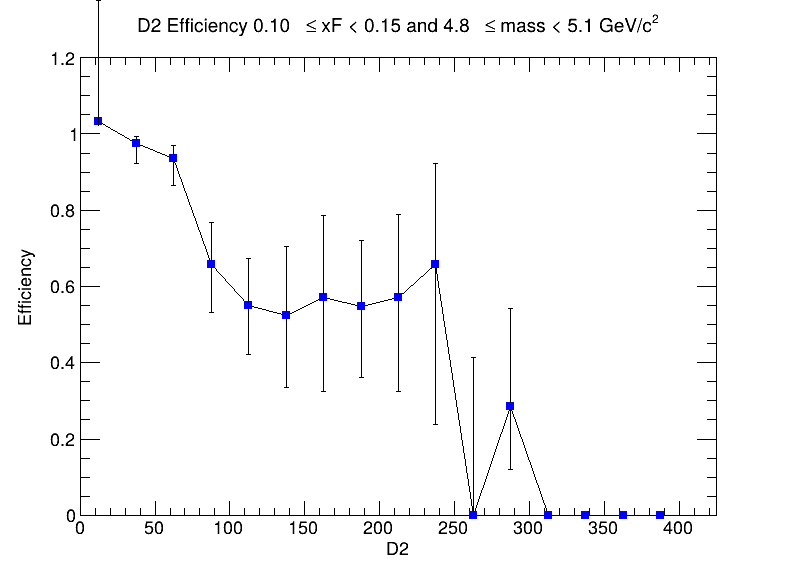
\includegraphics[width=\textwidth]{./kTrackerEfficiencyPlots/D2_Efficiency_xF2_mass2.png}
        \caption{$4.8 \leq m < 5.1$ GeV/$c^2$}
        \label{fig:xF2_mass2}
    \end{subfigure}
    \vspace{0.5cm}
    \begin{subfigure}[b]{0.32\textwidth}
        \centering
        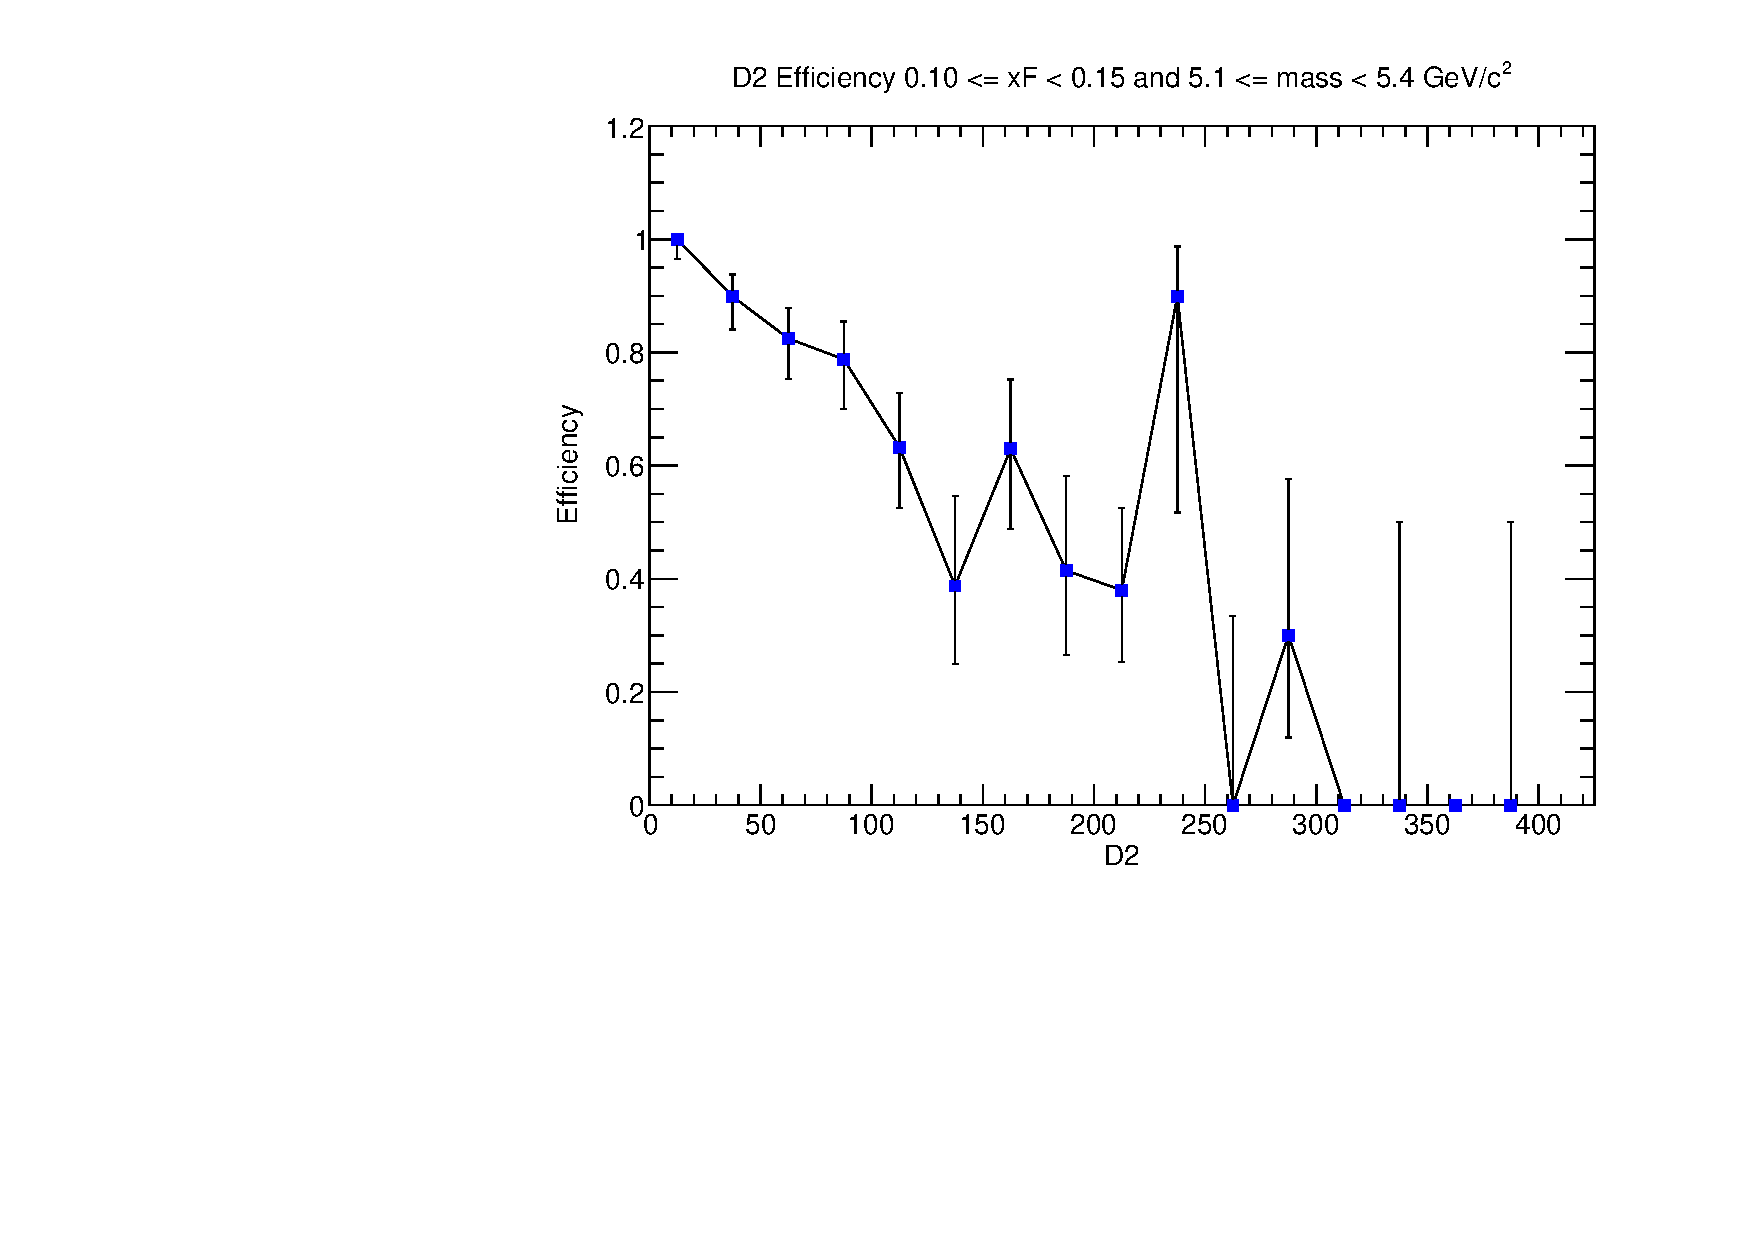
\includegraphics[width=\textwidth]{./kTrackerEfficiencyPlots/D2_Efficiency_xF2_mass3.pdf}
        \caption{$5.1 \leq m < 5.4$ GeV/$c^2$}
        \label{fig:xF2_mass3}
    \end{subfigure}
    \hfill
    \begin{subfigure}[b]{0.32\textwidth}
        \centering
        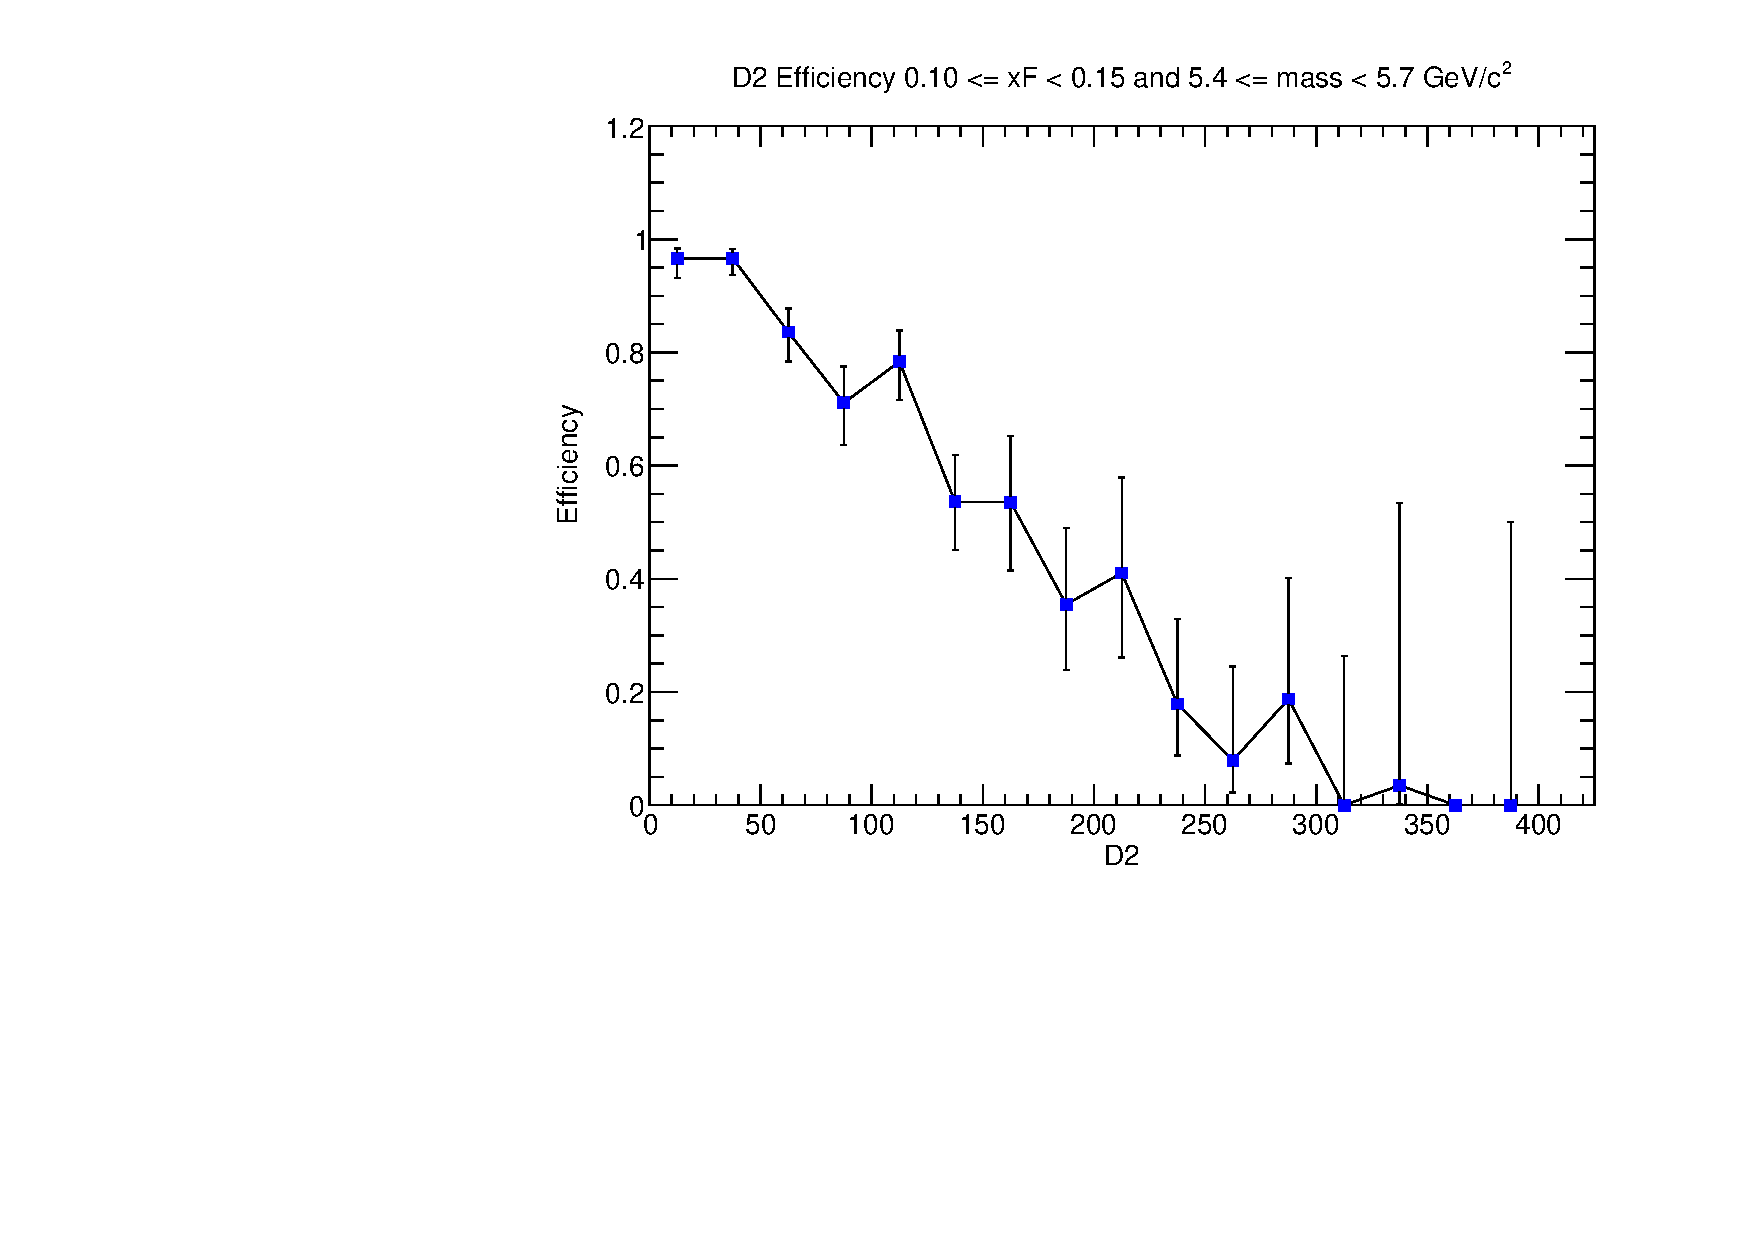
\includegraphics[width=\textwidth]{./kTrackerEfficiencyPlots/D2_Efficiency_xF2_mass4.pdf}
        \caption{$5.4 \leq m < 5.7$ GeV/$c^2$}
        \label{fig:xF2_mass4}
    \end{subfigure}
    \hfill
    \begin{subfigure}[b]{0.32\textwidth}
        \centering
        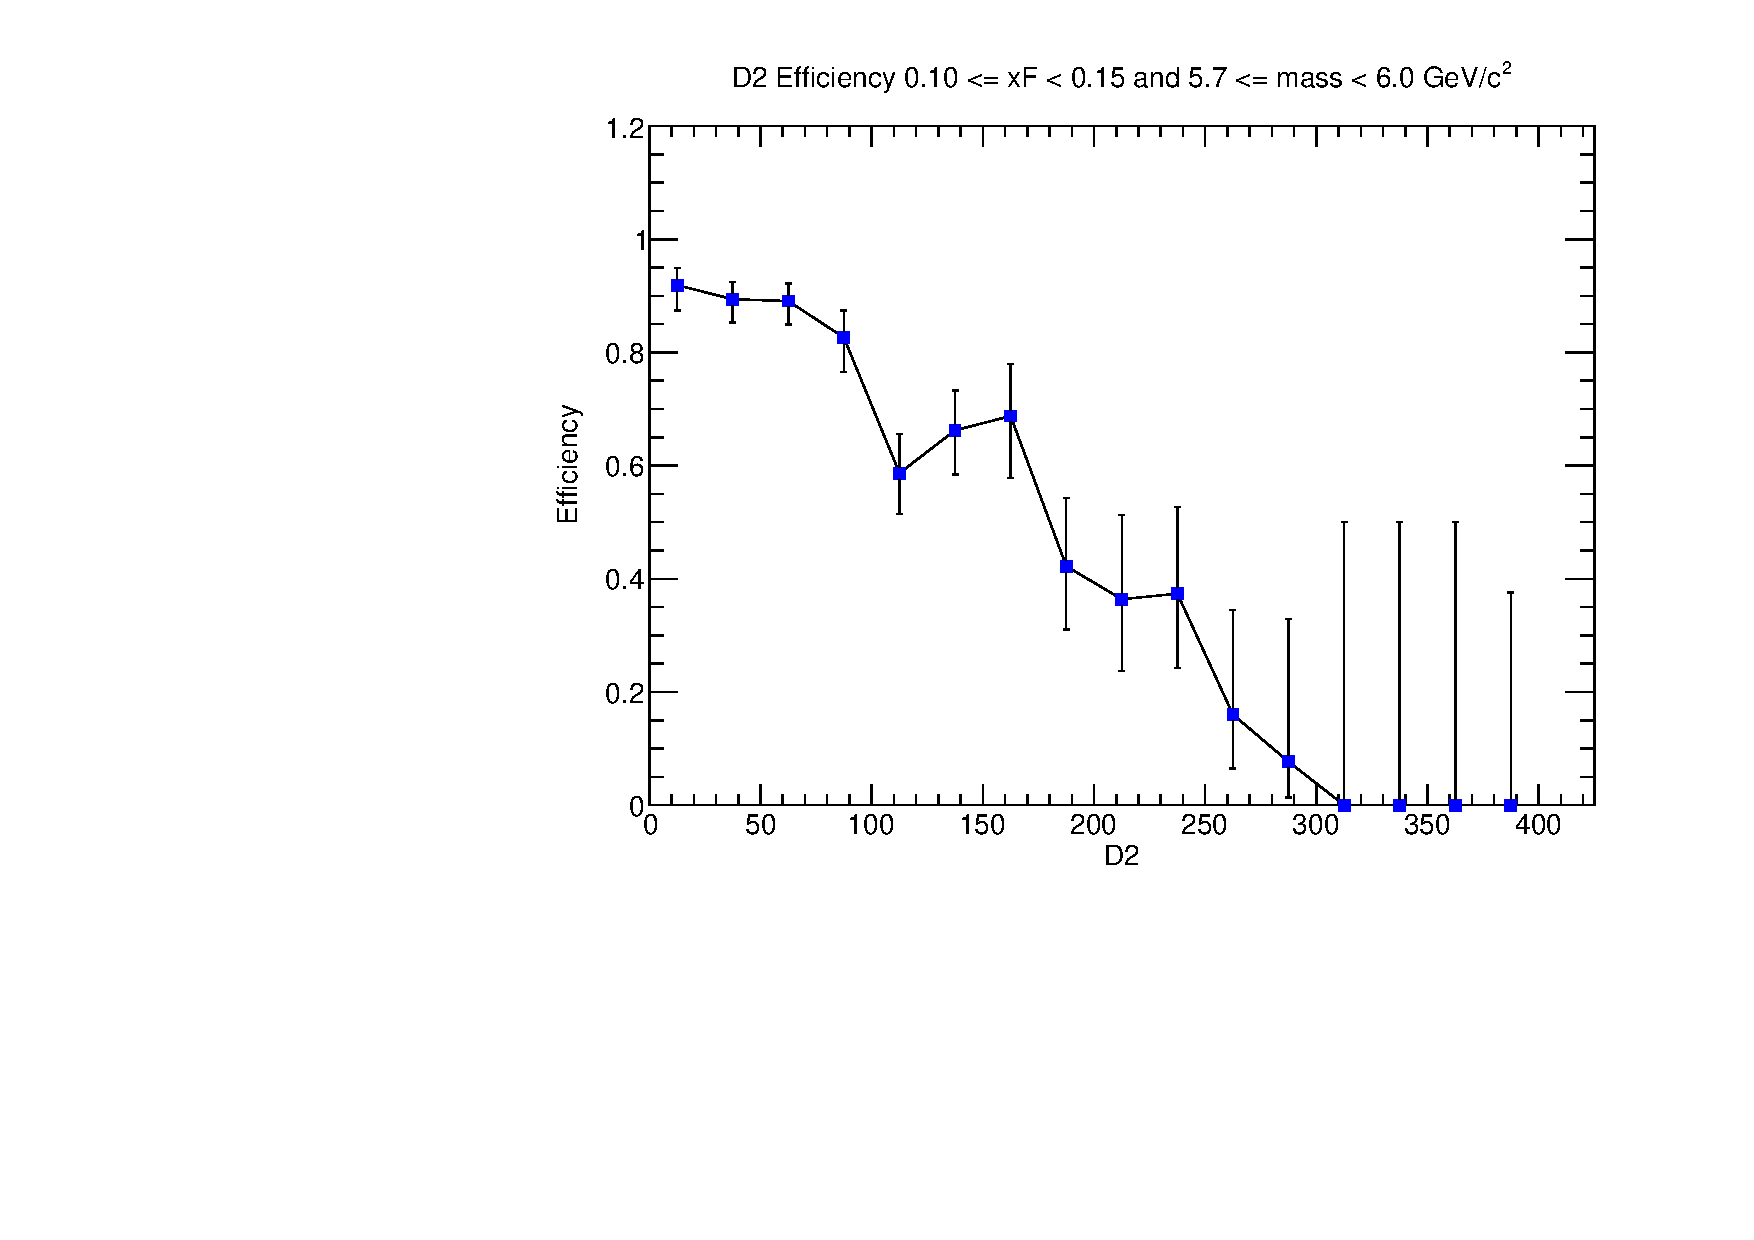
\includegraphics[width=\textwidth]{./kTrackerEfficiencyPlots/D2_Efficiency_xF2_mass5.pdf}
        \caption{$5.7 \leq m < 6.0$ GeV/$c^2$}
        \label{fig:xF2_mass5}
    \end{subfigure}
    \vspace{0.5cm}
    \begin{subfigure}[b]{0.32\textwidth}
        \centering
        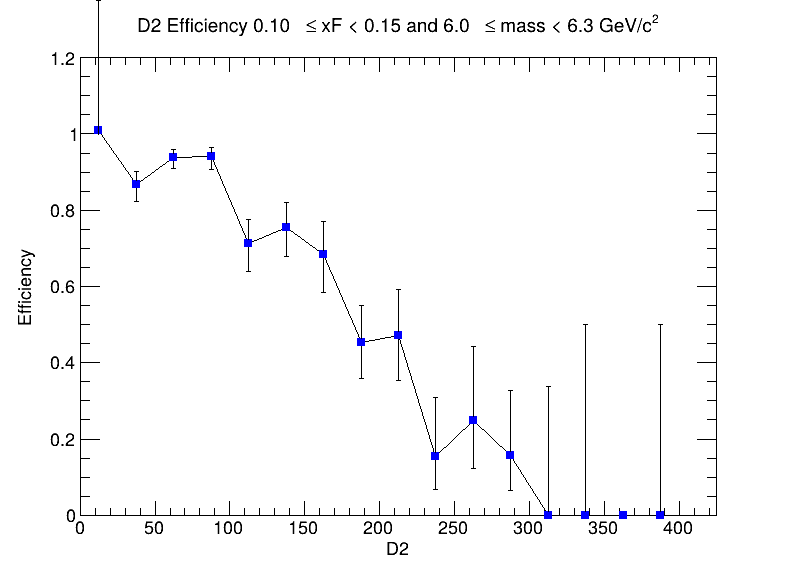
\includegraphics[width=\textwidth]{./kTrackerEfficiencyPlots/D2_Efficiency_xF2_mass6.png}
        \caption{$6.0 \leq m < 6.3$ GeV/$c^2$}
        \label{fig:xF2_mass6}
    \end{subfigure}
    \hfill
    \begin{subfigure}[b]{0.32\textwidth}
        \centering
        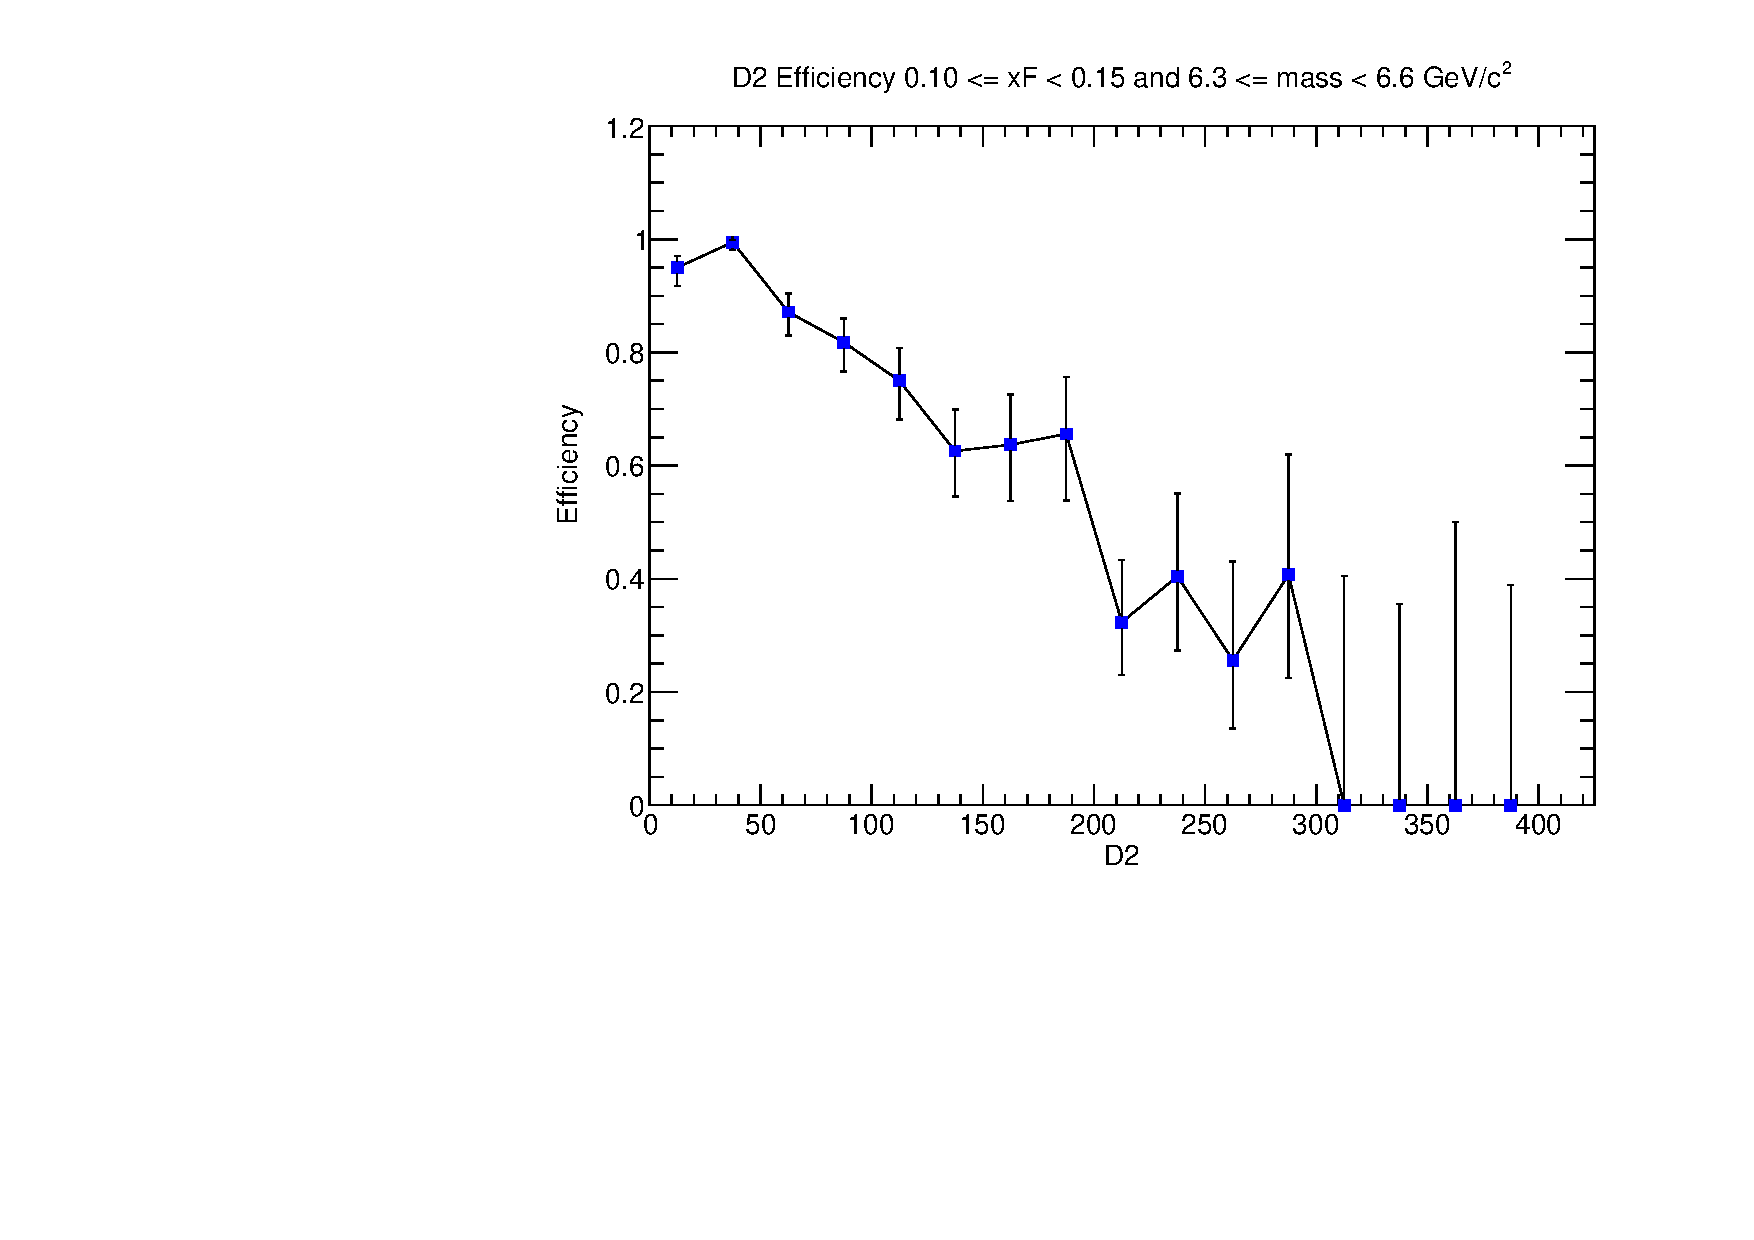
\includegraphics[width=\textwidth]{./kTrackerEfficiencyPlots/D2_Efficiency_xF2_mass7.pdf}
        \caption{$6.3 \leq m < 6.6$ GeV/$c^2$}
        \label{fig:xF2_mass7}
    \end{subfigure}
    \hfill
    \begin{subfigure}[b]{0.32\textwidth}
        \centering
        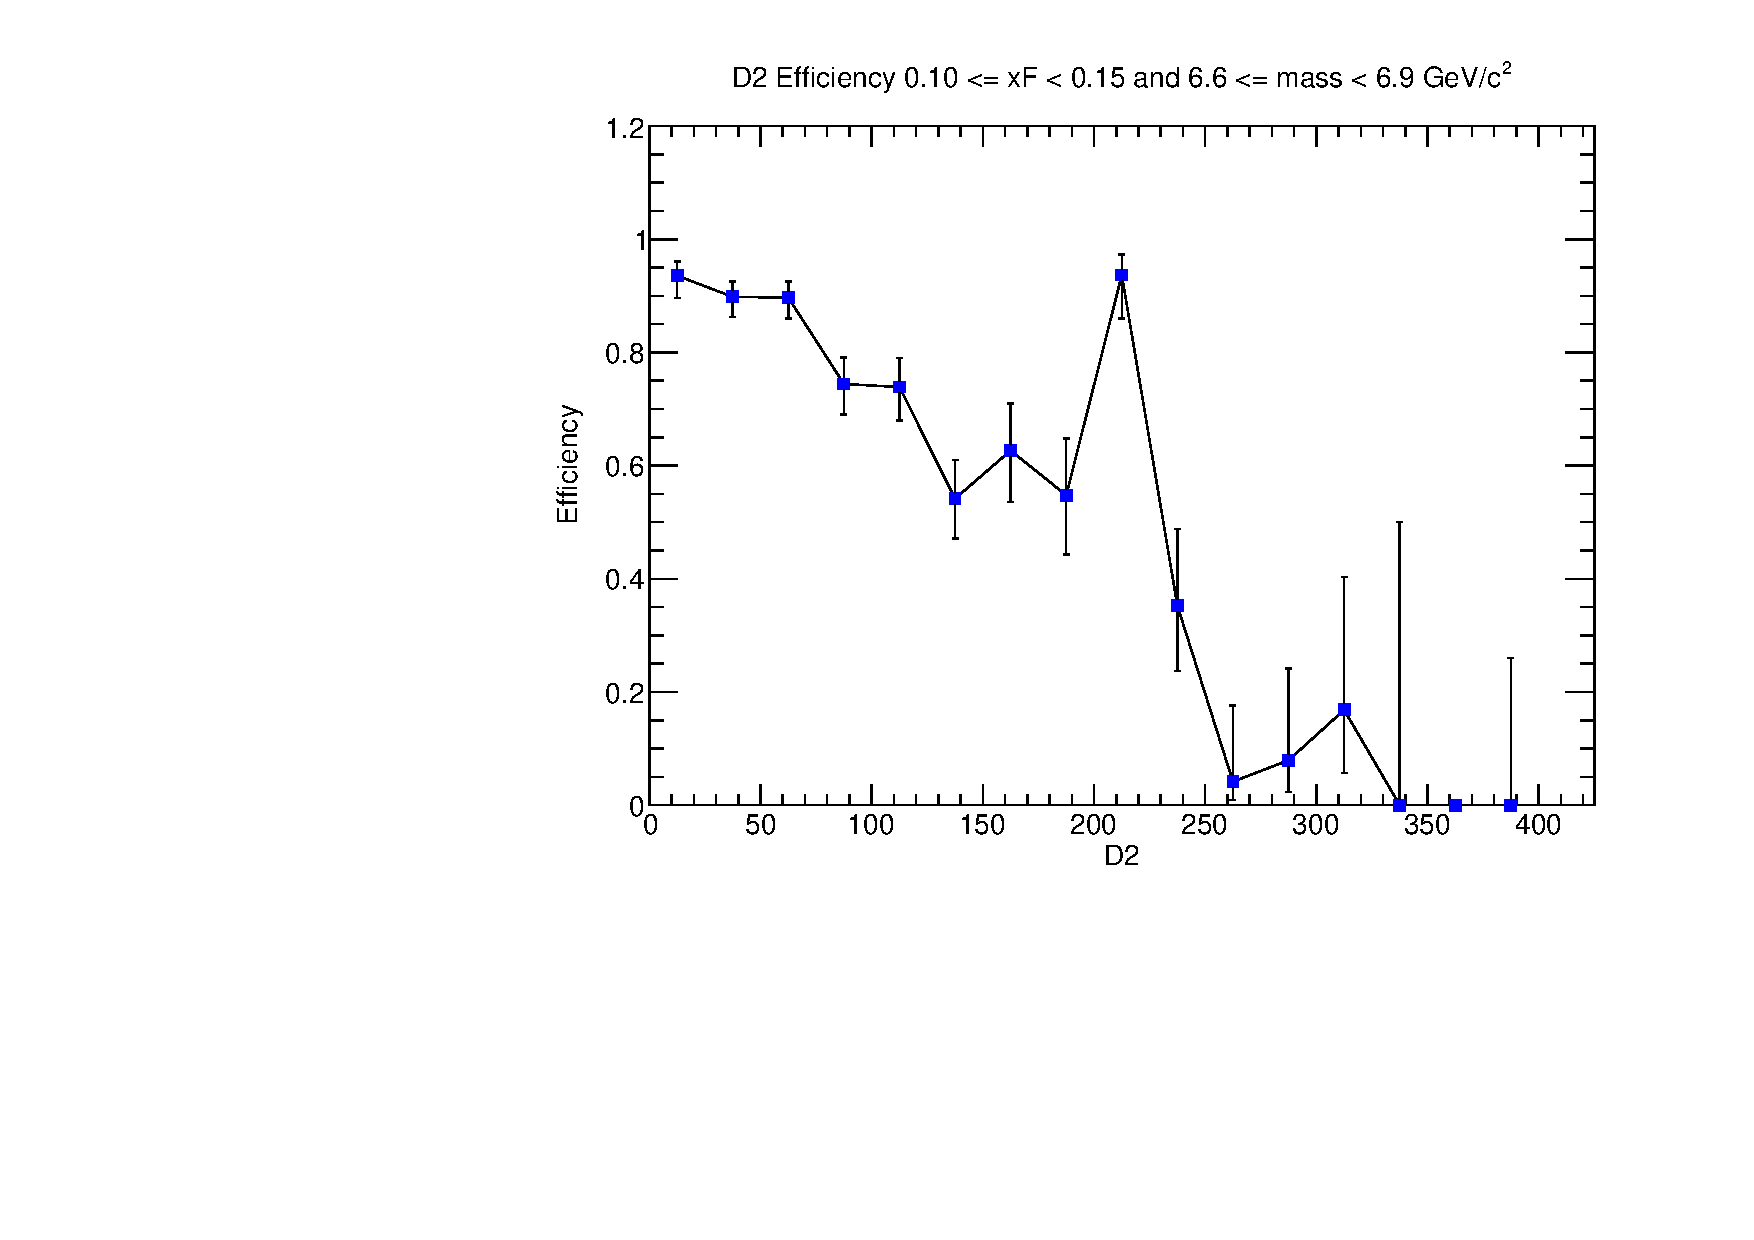
\includegraphics[width=\textwidth]{./kTrackerEfficiencyPlots/D2_Efficiency_xF2_mass8.pdf}
        \caption{$6.6 \leq m < 6.9$ GeV/$c^2$}
        \label{fig:xF2_mass8}
    \end{subfigure}
    \vspace{0.5cm}
    \begin{subfigure}[b]{0.32\textwidth}
        \centering
        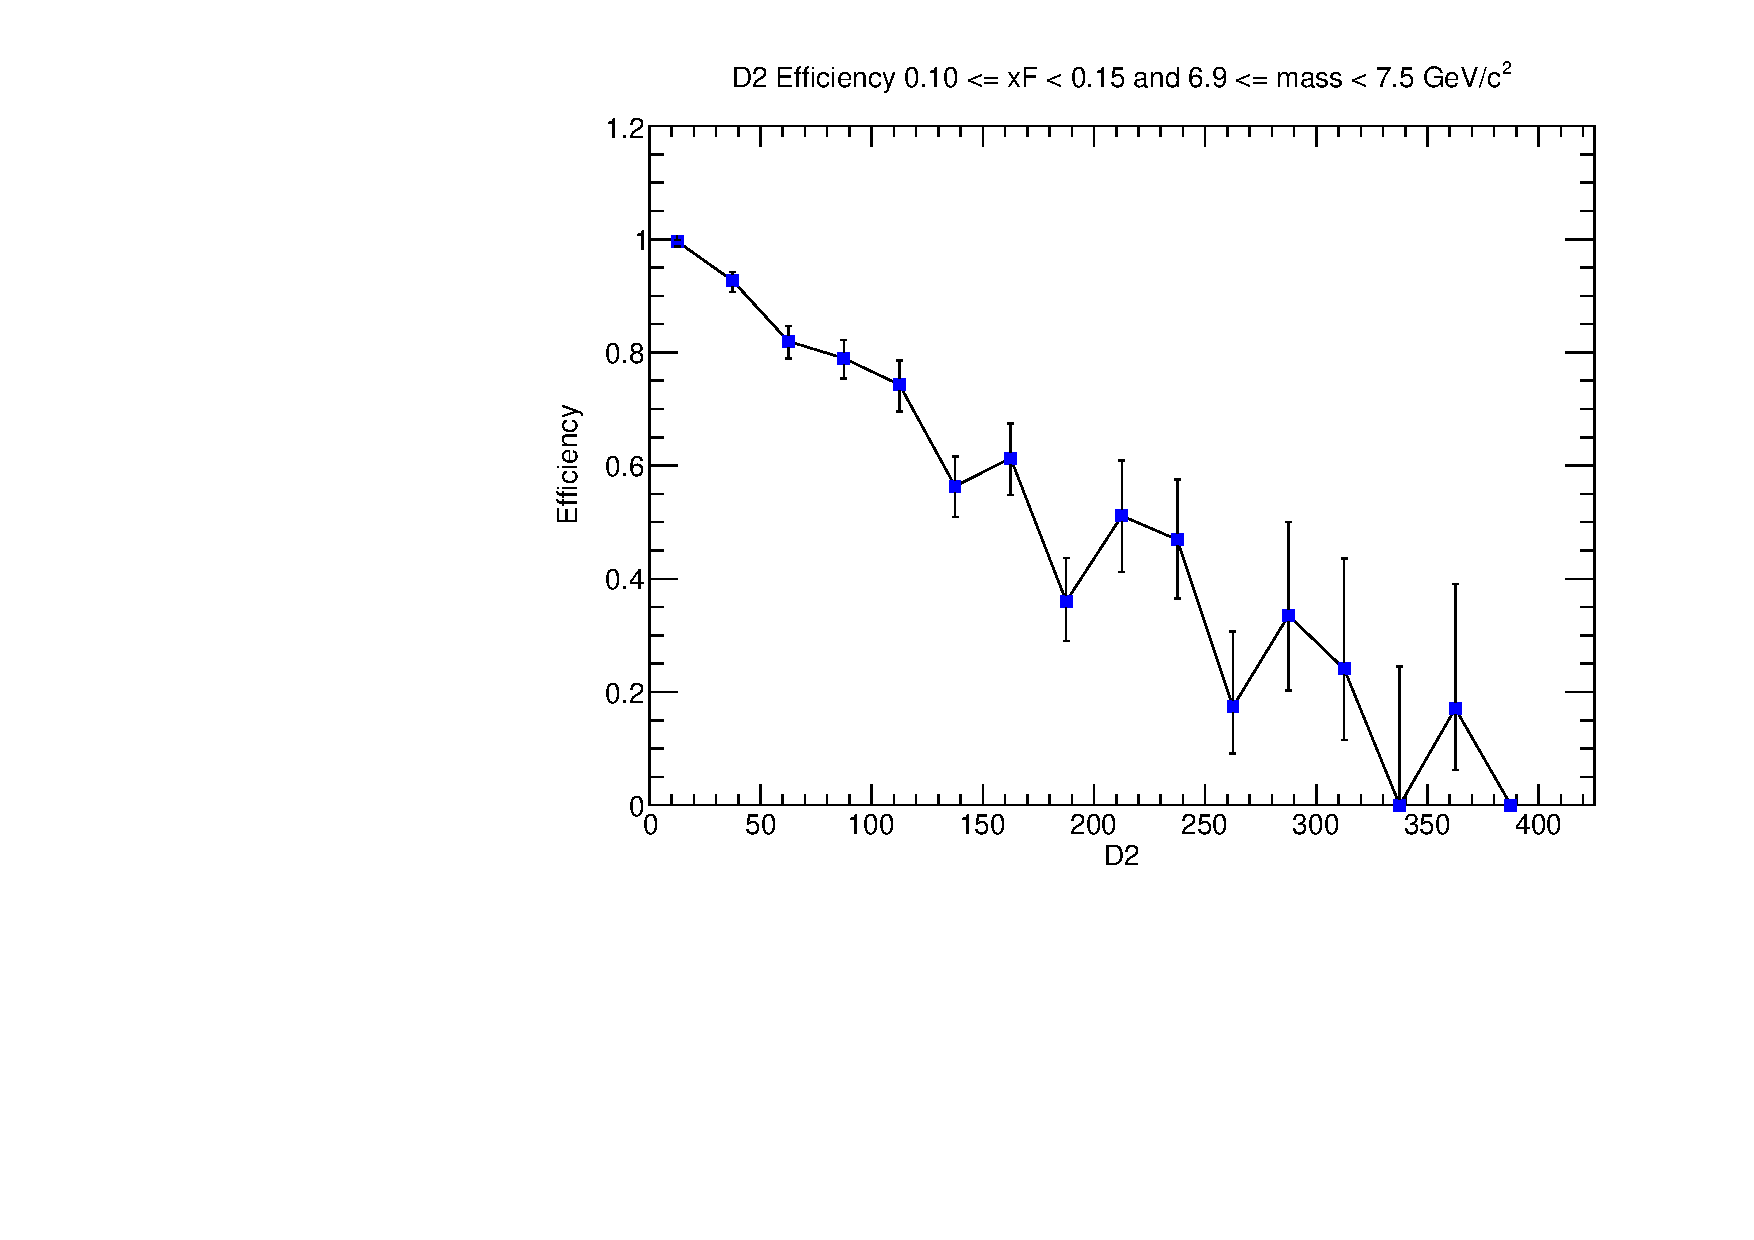
\includegraphics[width=\textwidth]{./kTrackerEfficiencyPlots/D2_Efficiency_xF2_mass9.pdf}
        \caption{$6.9 \leq m < 7.5$ GeV/$c^2$}
        \label{fig:xF2_mass9}
    \end{subfigure}
    \hfill
    \begin{subfigure}[b]{0.32\textwidth}
        \centering
        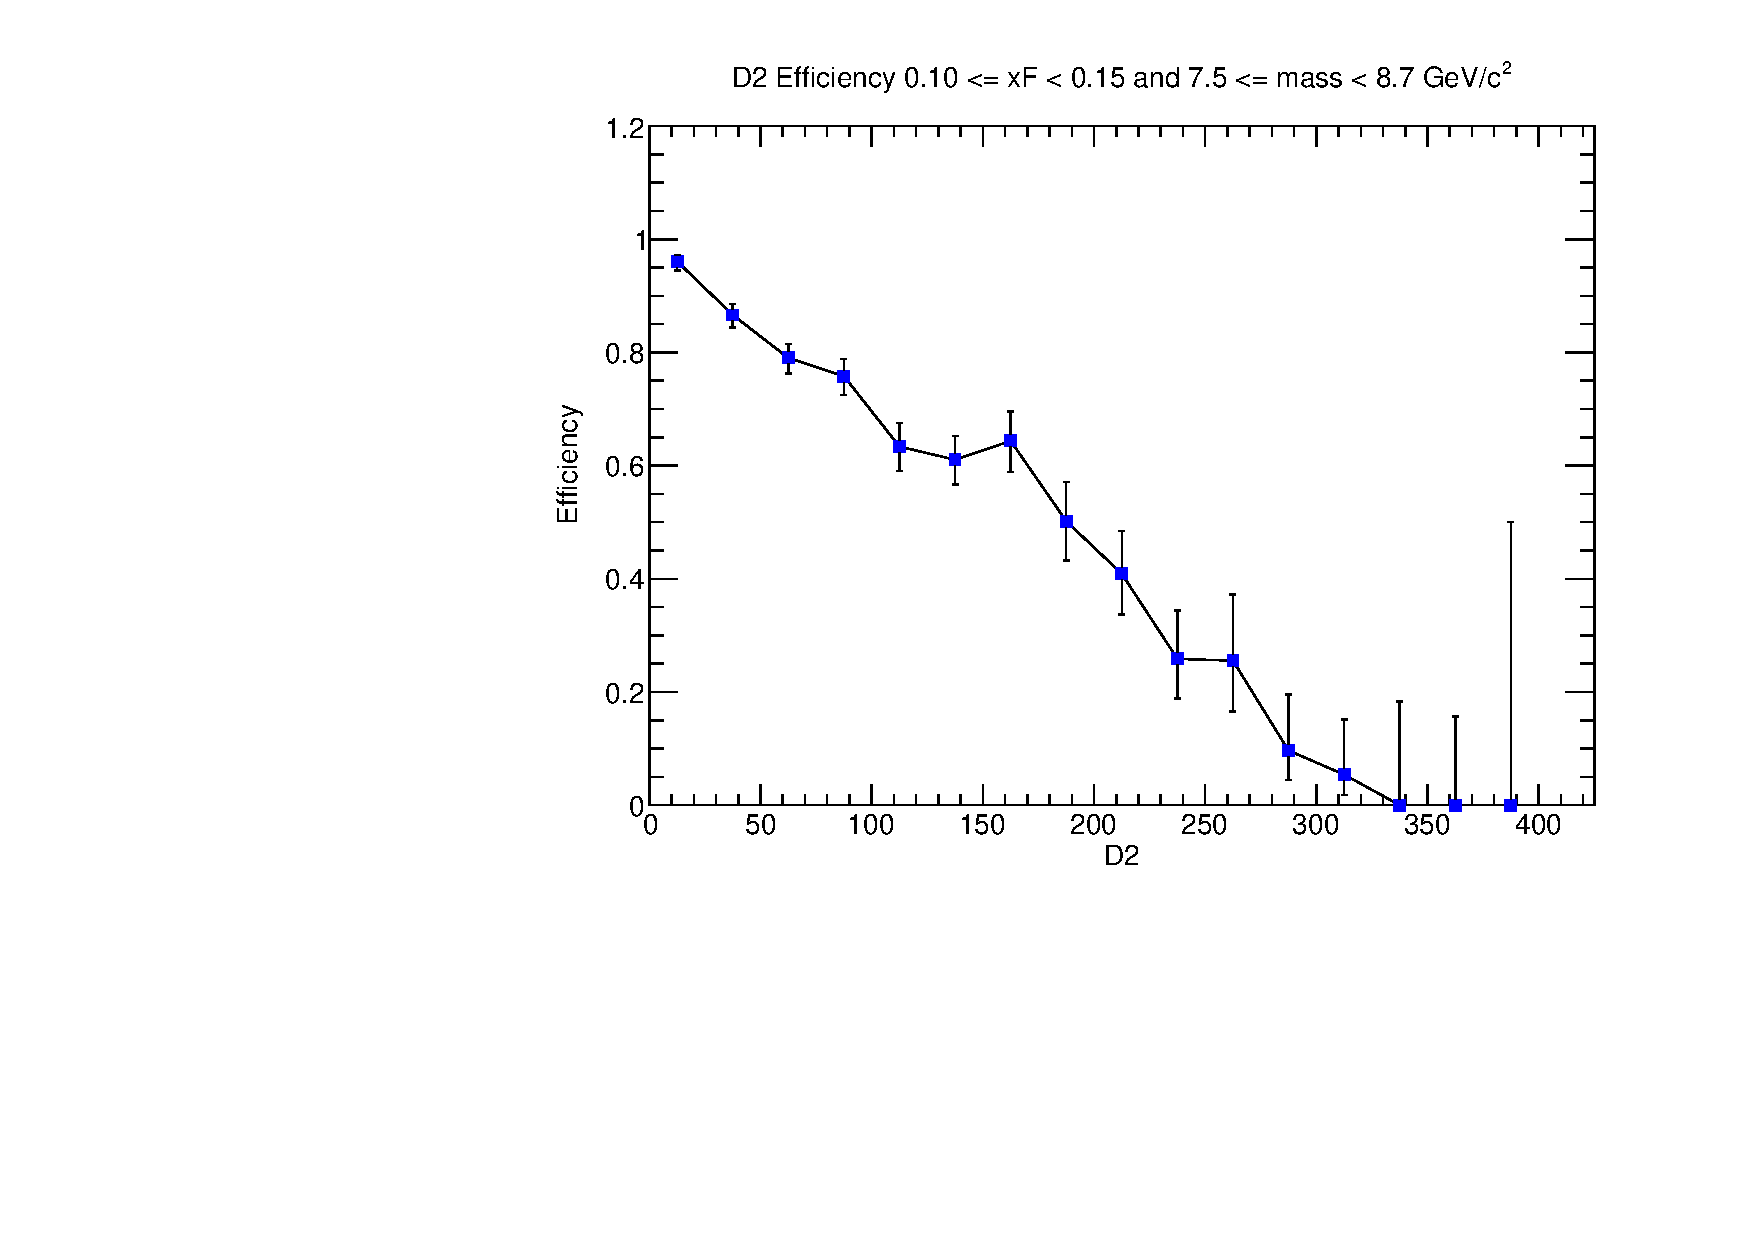
\includegraphics[width=\textwidth]{./kTrackerEfficiencyPlots/D2_Efficiency_xF2_mass10.pdf}
        \caption{$7.5 \leq m < 8.7$ GeV/$c^2$}
        \label{fig:xF2_mass10}
    \end{subfigure}
    \hfill
    \caption{Efficiency plots for the $x_F$ bin $0.10 \leq x_F < 0.15$.}
    \label{fig:xF2}
\end{figure}

\clearpage

\begin{figure}[p]
    \centering
    \begin{subfigure}[b]{0.32\textwidth}
        \centering
        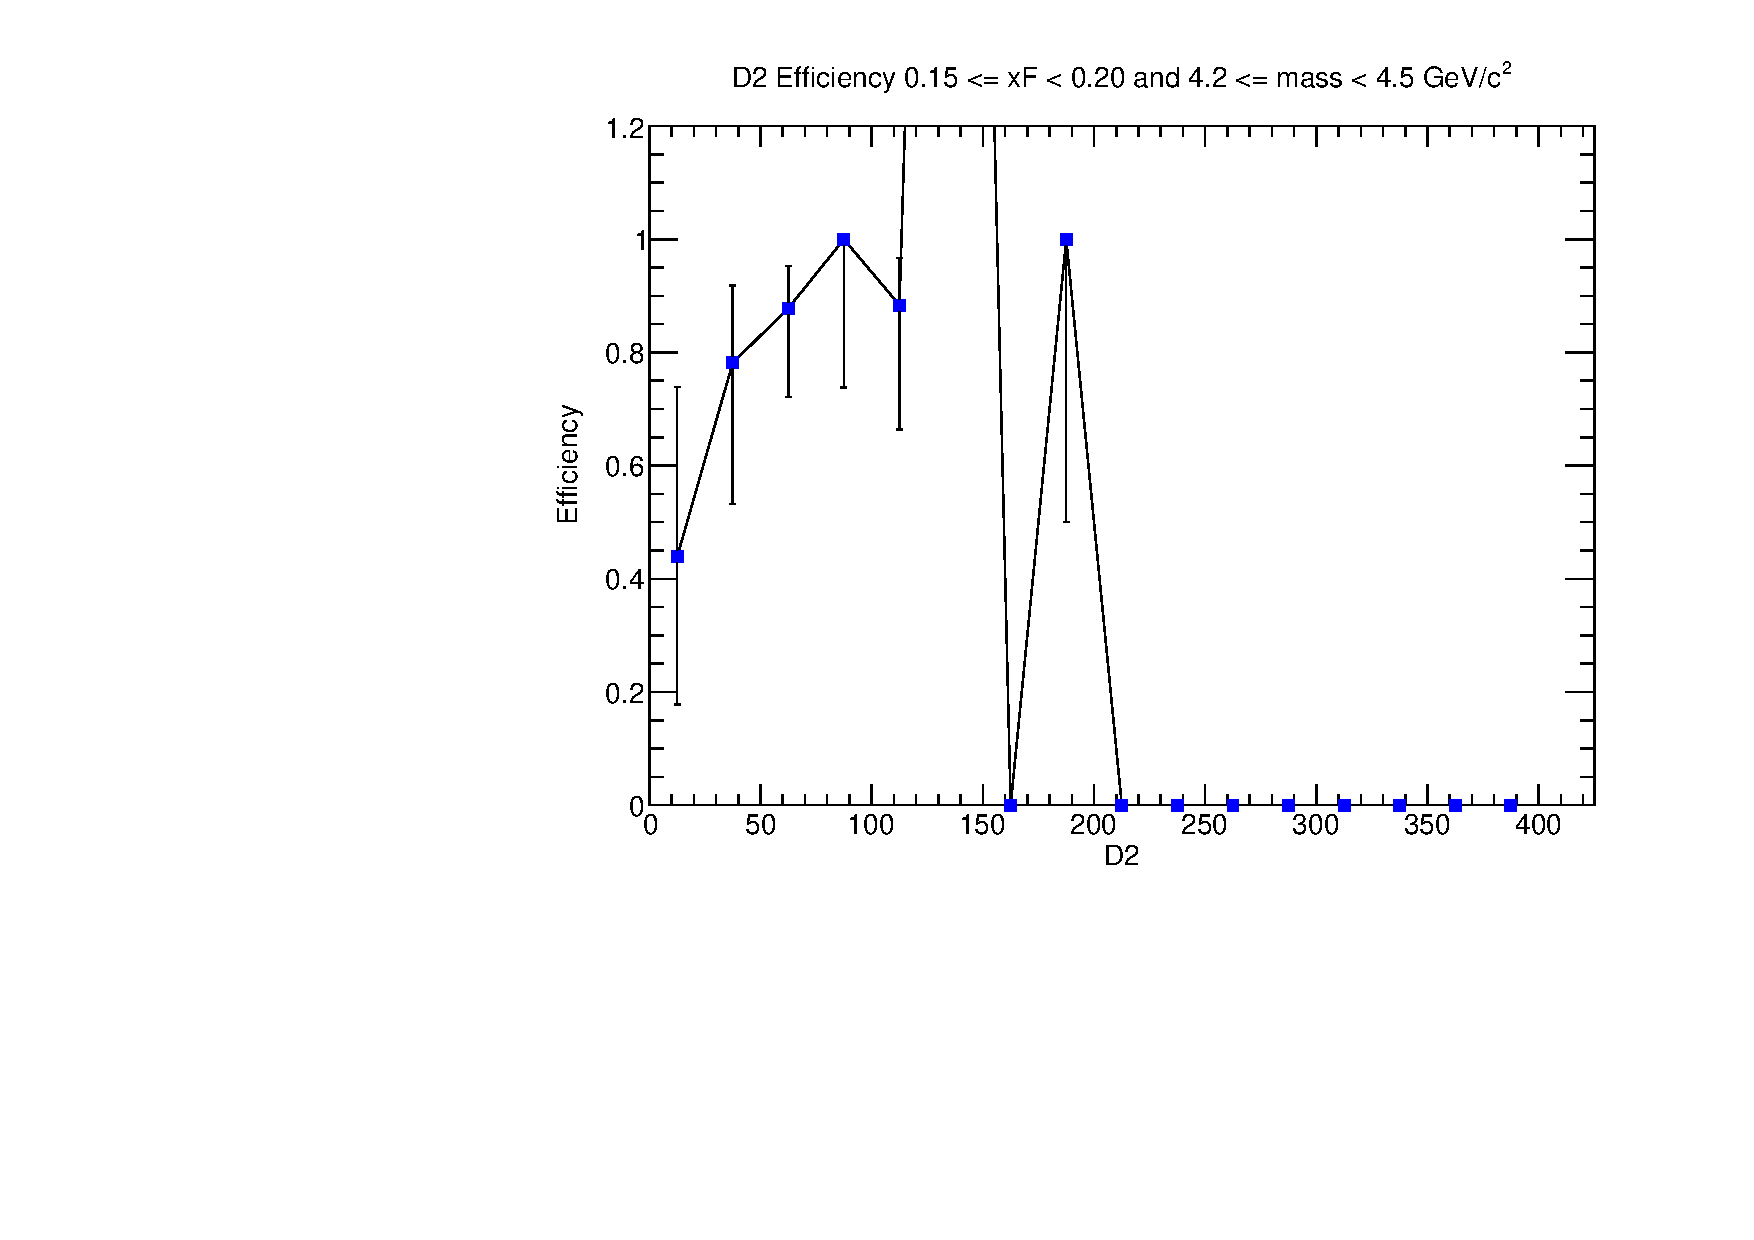
\includegraphics[width=\textwidth]{./kTrackerEfficiencyPlots/D2_Efficiency_xF3_mass0.pdf}
        \caption{$4.2 \leq m < 4.5$ GeV/$c^2$}
        \label{fig:xF3_mass0}
    \end{subfigure}
    \hfill
    \begin{subfigure}[b]{0.32\textwidth}
        \centering
        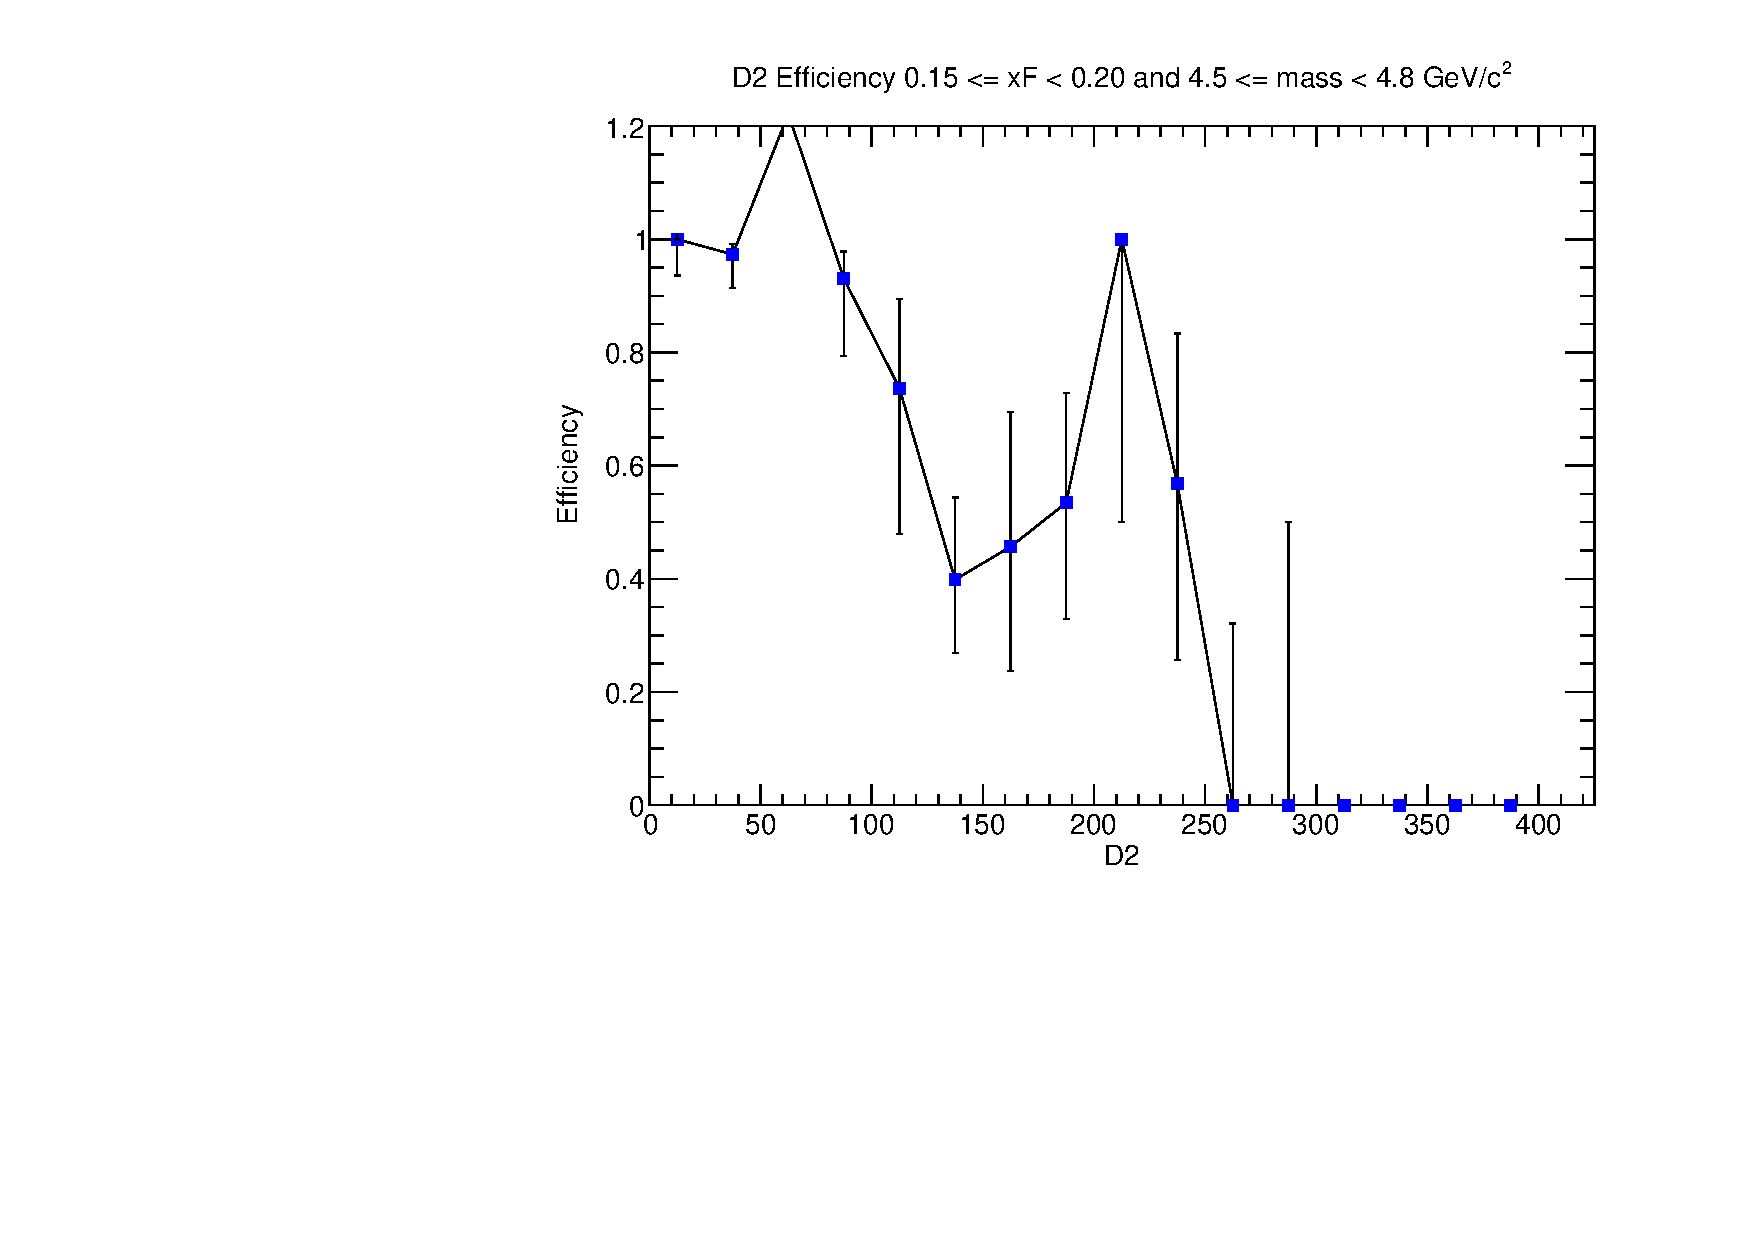
\includegraphics[width=\textwidth]{./kTrackerEfficiencyPlots/D2_Efficiency_xF3_mass1.pdf}
        \caption{$4.5 \leq m < 4.8$ GeV/$c^2$}
        \label{fig:xF3_mass1}
    \end{subfigure}
    \hfill
    \begin{subfigure}[b]{0.32\textwidth}
        \centering
        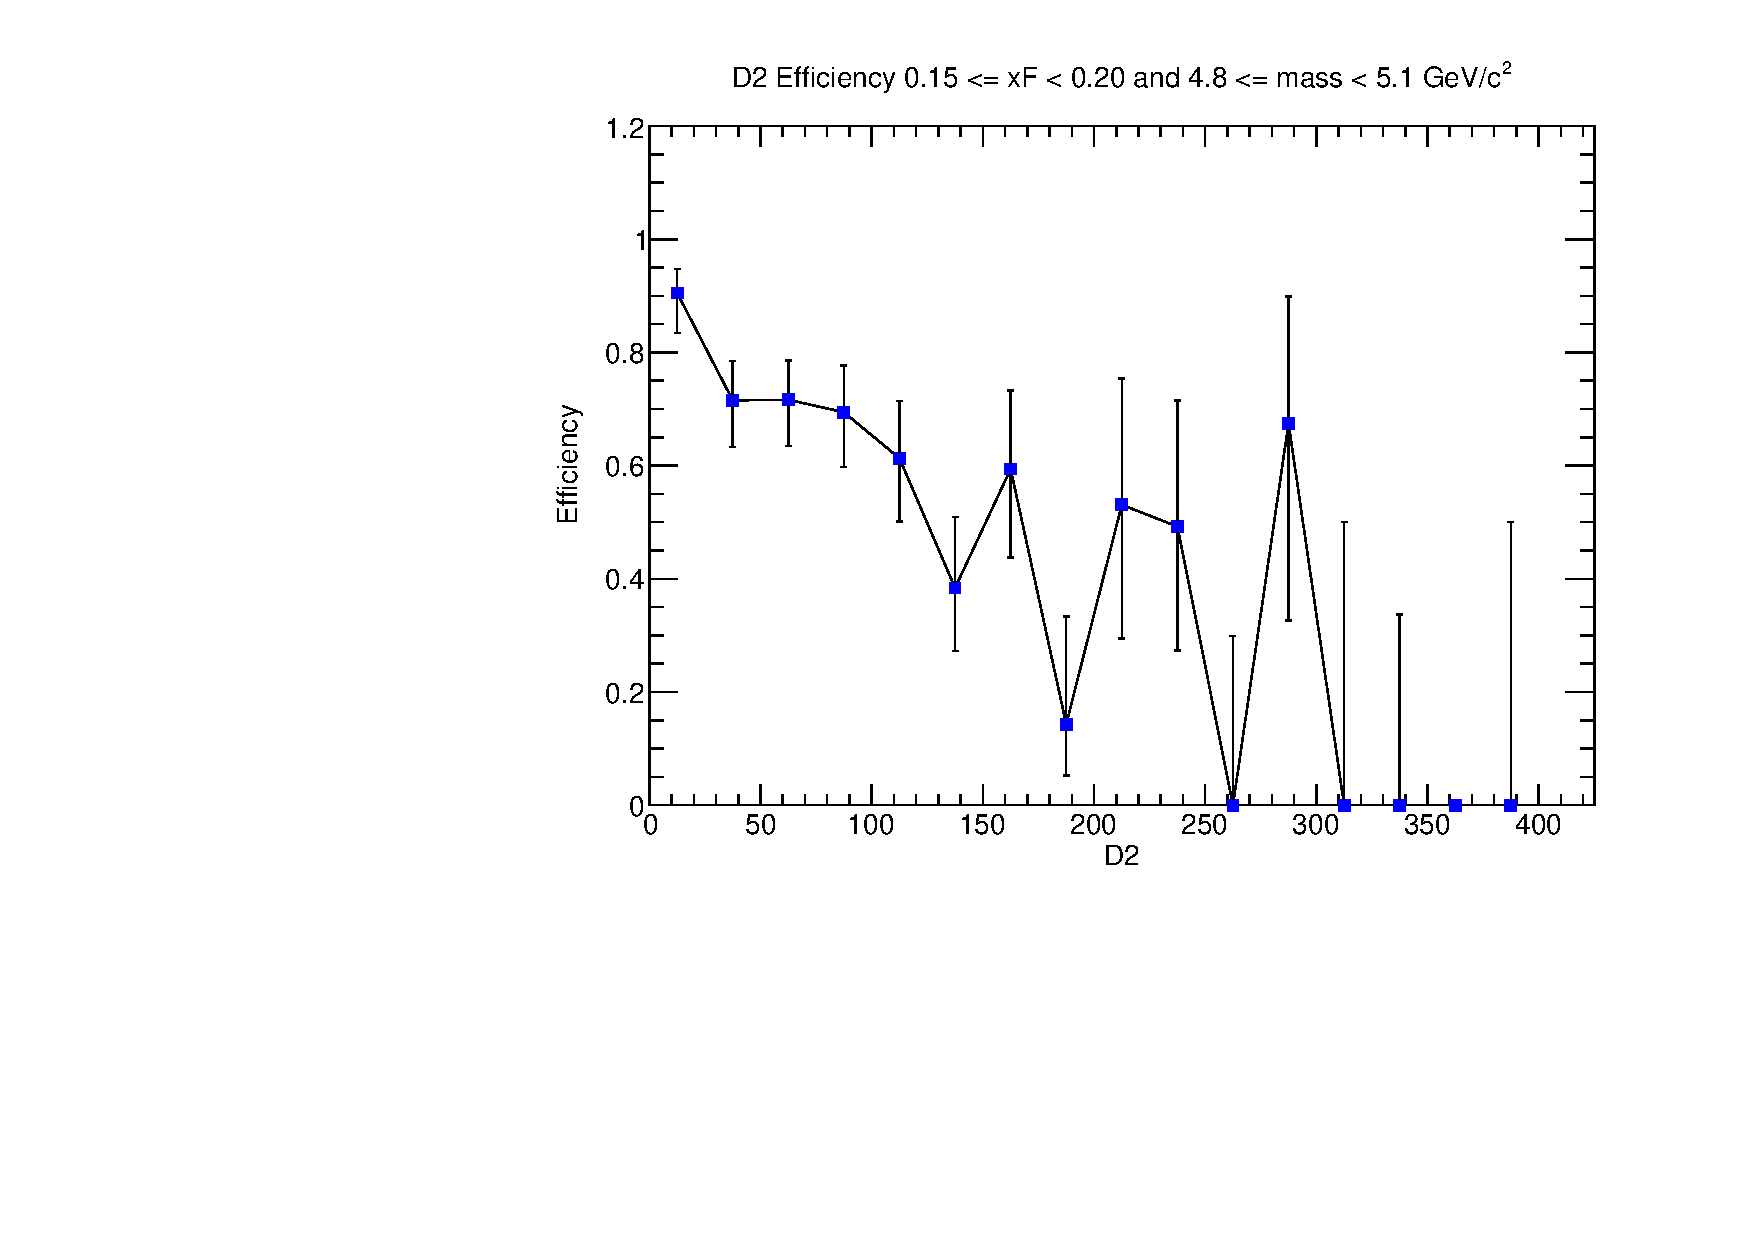
\includegraphics[width=\textwidth]{./kTrackerEfficiencyPlots/D2_Efficiency_xF3_mass2.pdf}
        \caption{$4.8 \leq m < 5.1$ GeV/$c^2$}
        \label{fig:xF3_mass2}
    \end{subfigure}
    \vspace{0.5cm}
    \begin{subfigure}[b]{0.32\textwidth}
        \centering
        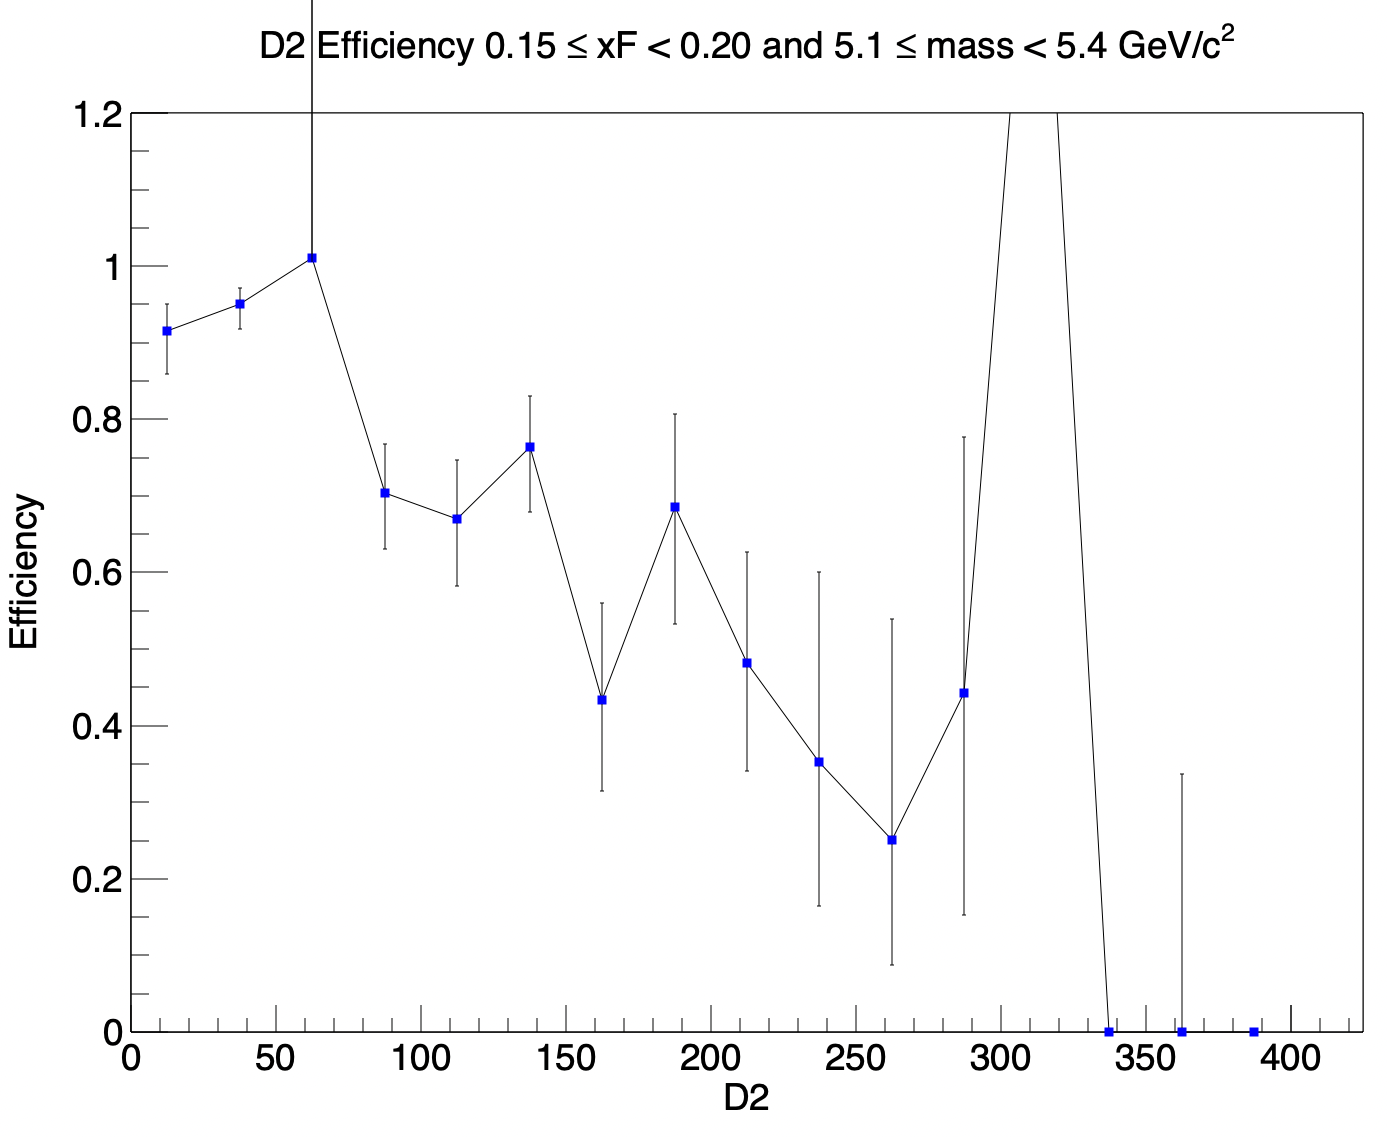
\includegraphics[width=\textwidth]{./kTrackerEfficiencyPlots/D2_Efficiency_xF3_mass3.png}
        \caption{$5.1 \leq m < 5.4$ GeV/$c^2$}
        \label{fig:xF3_mass3}
    \end{subfigure}
    \hfill
    \begin{subfigure}[b]{0.32\textwidth}
        \centering
        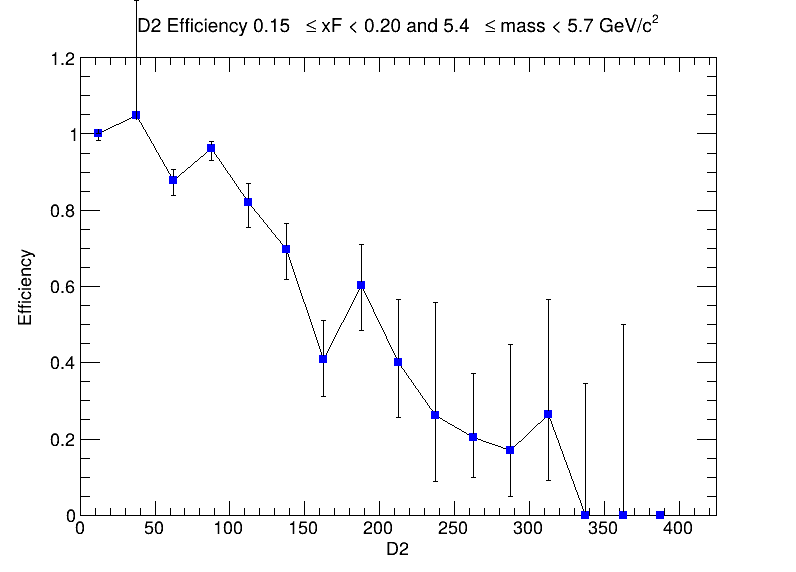
\includegraphics[width=\textwidth]{./kTrackerEfficiencyPlots/D2_Efficiency_xF3_mass4.png}
        \caption{$5.4 \leq m < 5.7$ GeV/$c^2$}
        \label{fig:xF3_mass4}
    \end{subfigure}
    \hfill
    \begin{subfigure}[b]{0.32\textwidth}
        \centering
        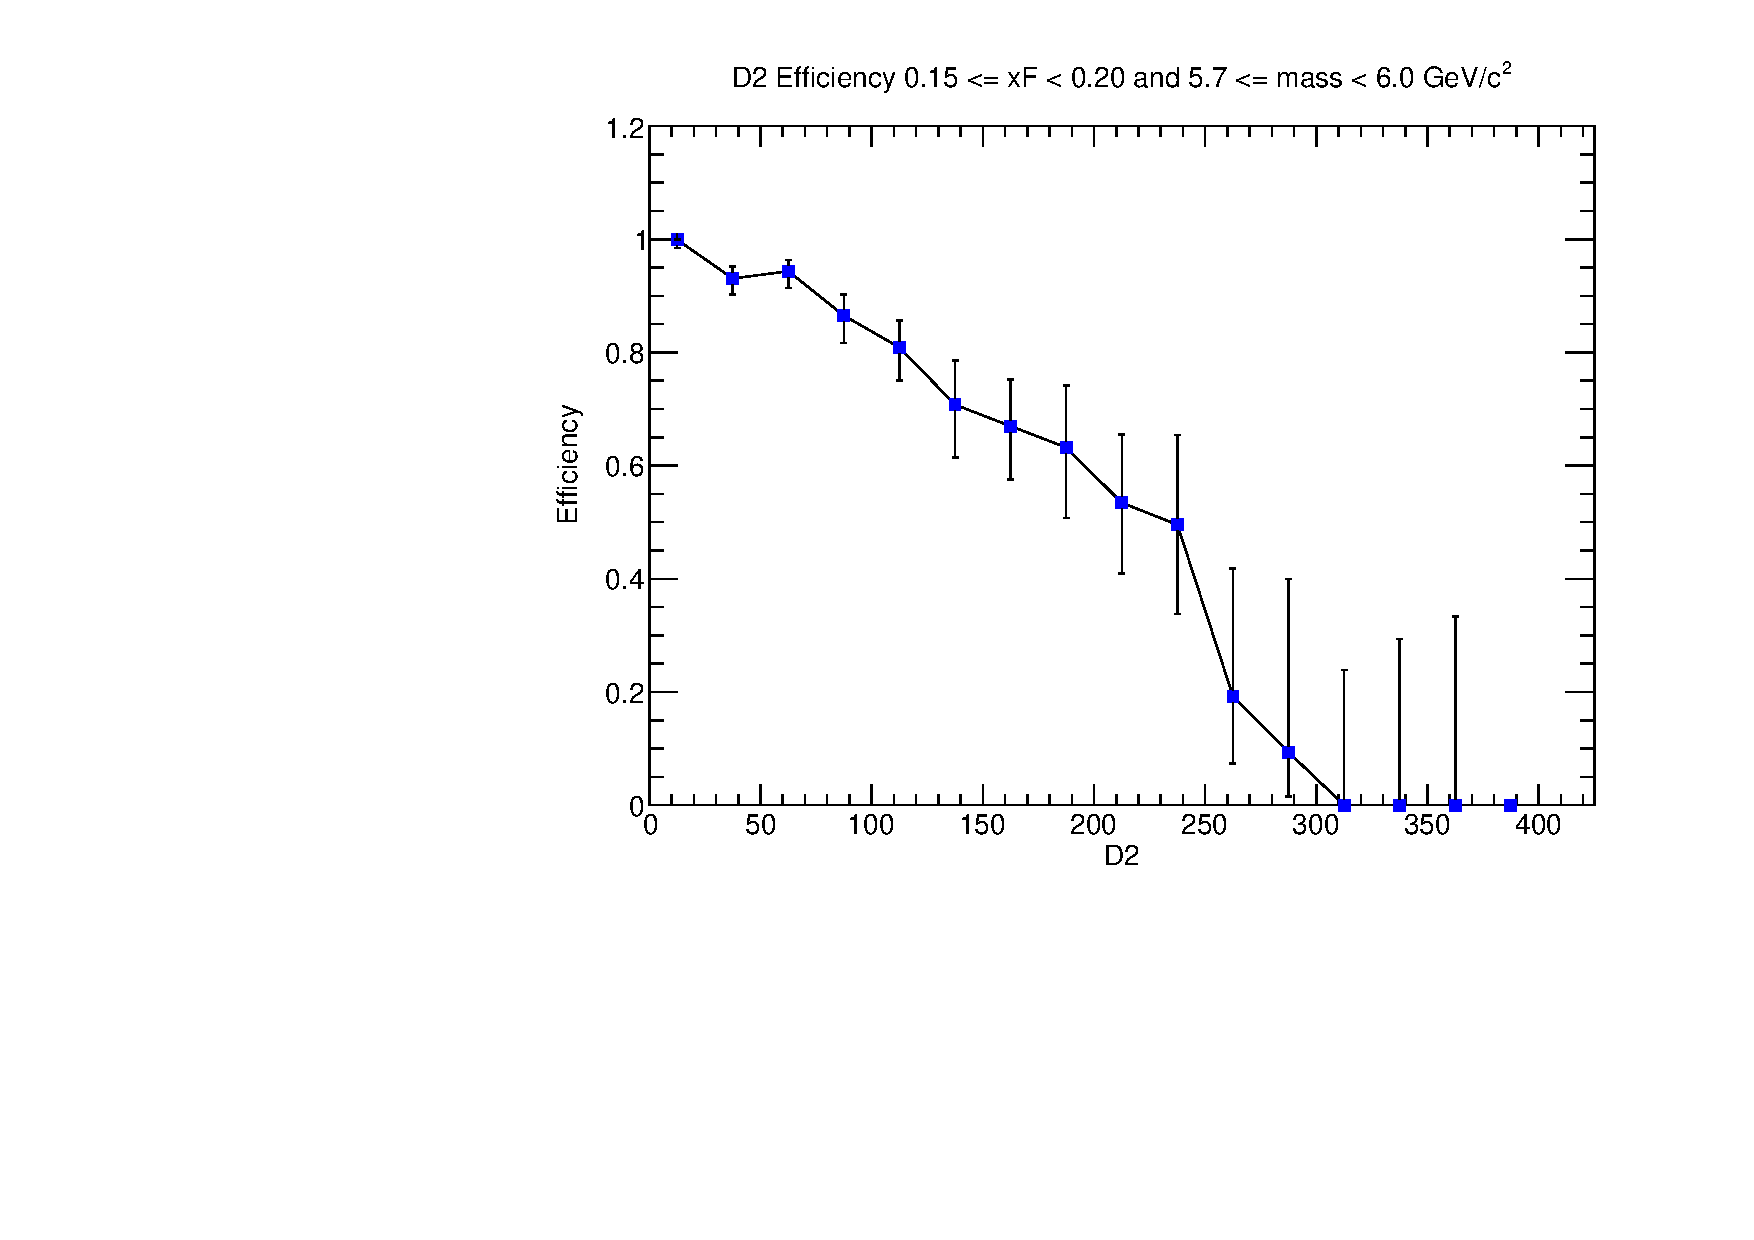
\includegraphics[width=\textwidth]{./kTrackerEfficiencyPlots/D2_Efficiency_xF3_mass5.pdf}
        \caption{$5.7 \leq m < 6.0$ GeV/$c^2$}
        \label{fig:xF3_mass5}
    \end{subfigure}
    \vspace{0.5cm}
    \begin{subfigure}[b]{0.32\textwidth}
        \centering
        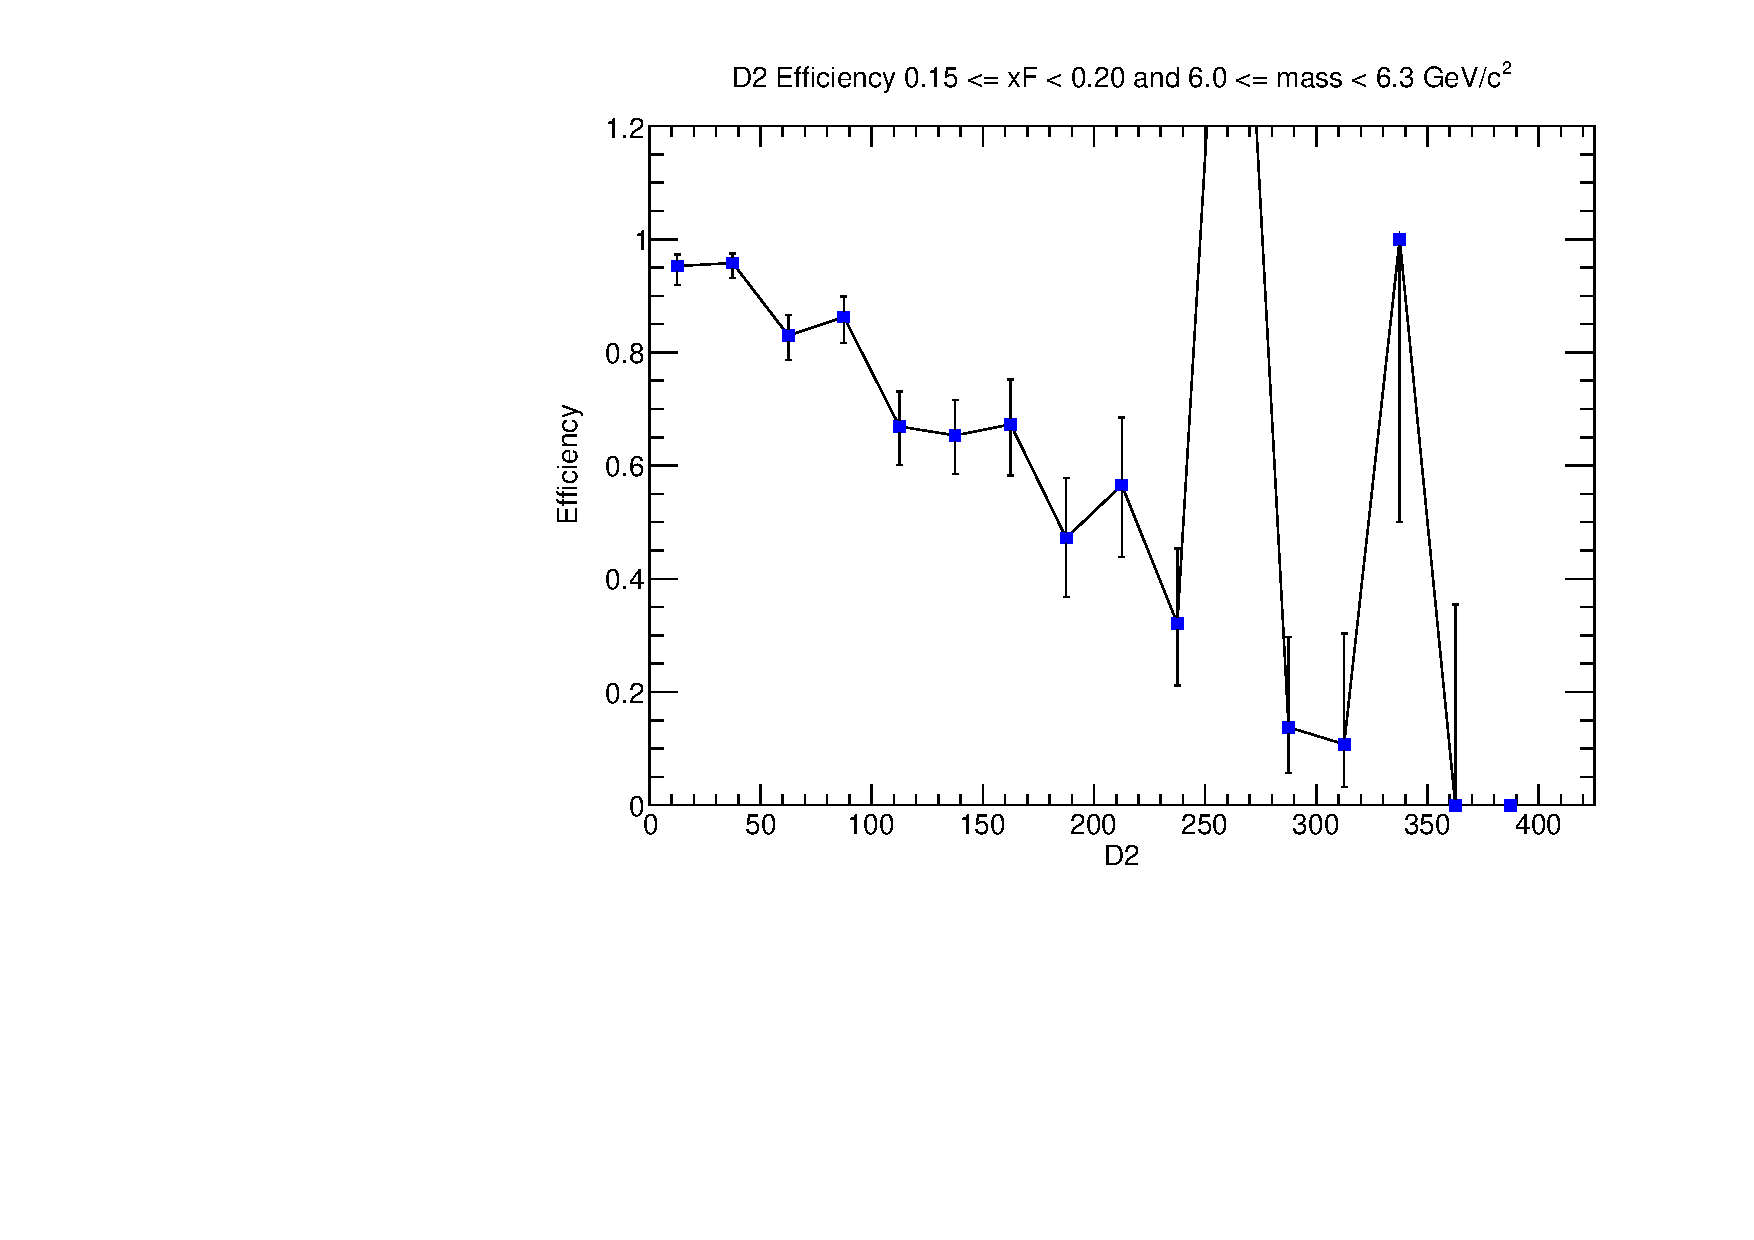
\includegraphics[width=\textwidth]{./kTrackerEfficiencyPlots/D2_Efficiency_xF3_mass6.pdf}
        \caption{$6.0 \leq m < 6.3$ GeV/$c^2$}
        \label{fig:xF3_mass6}
    \end{subfigure}
    \hfill
    \begin{subfigure}[b]{0.32\textwidth}
        \centering
        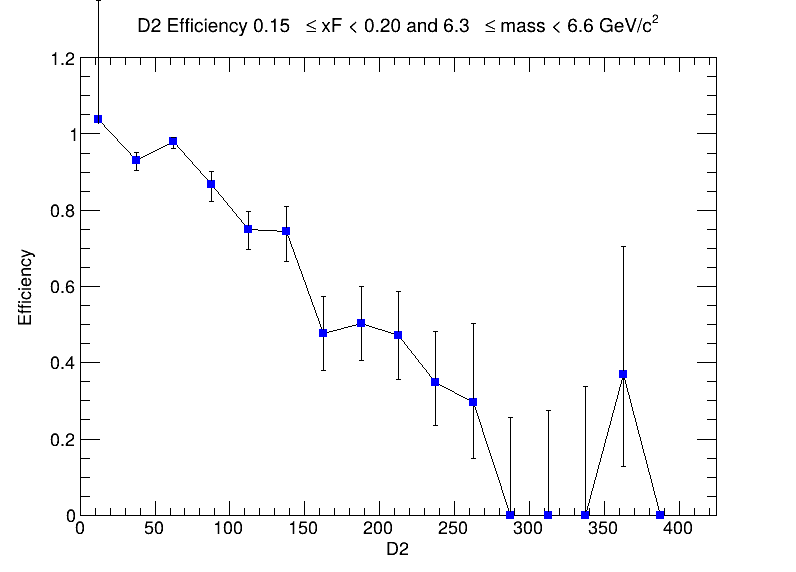
\includegraphics[width=\textwidth]{./kTrackerEfficiencyPlots/D2_Efficiency_xF3_mass7.png}
        \caption{$6.3 \leq m < 6.6$ GeV/$c^2$}
        \label{fig:xF3_mass7}
    \end{subfigure}
    \hfill
    \begin{subfigure}[b]{0.32\textwidth}
        \centering
        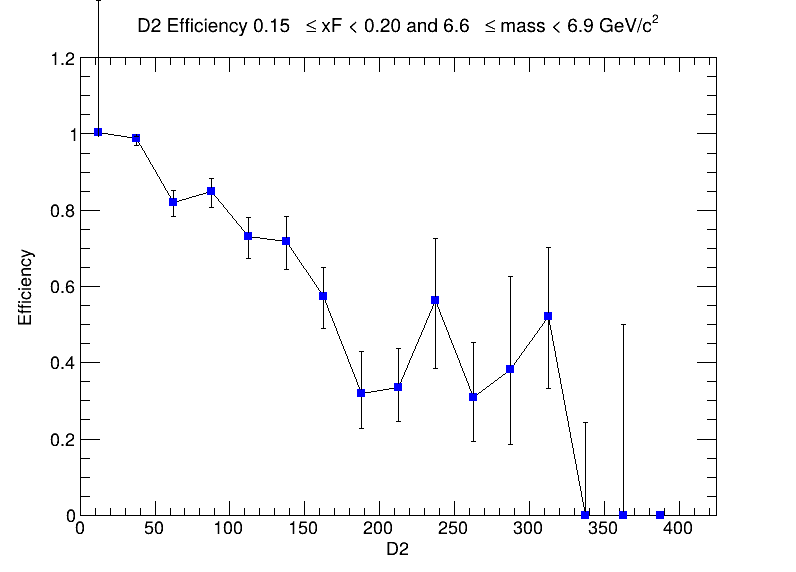
\includegraphics[width=\textwidth]{./kTrackerEfficiencyPlots/D2_Efficiency_xF3_mass8.png}
        \caption{$6.6 \leq m < 6.9$ GeV/$c^2$}
        \label{fig:xF3_mass8}
    \end{subfigure}
    \vspace{0.5cm}
    \begin{subfigure}[b]{0.32\textwidth}
        \centering
        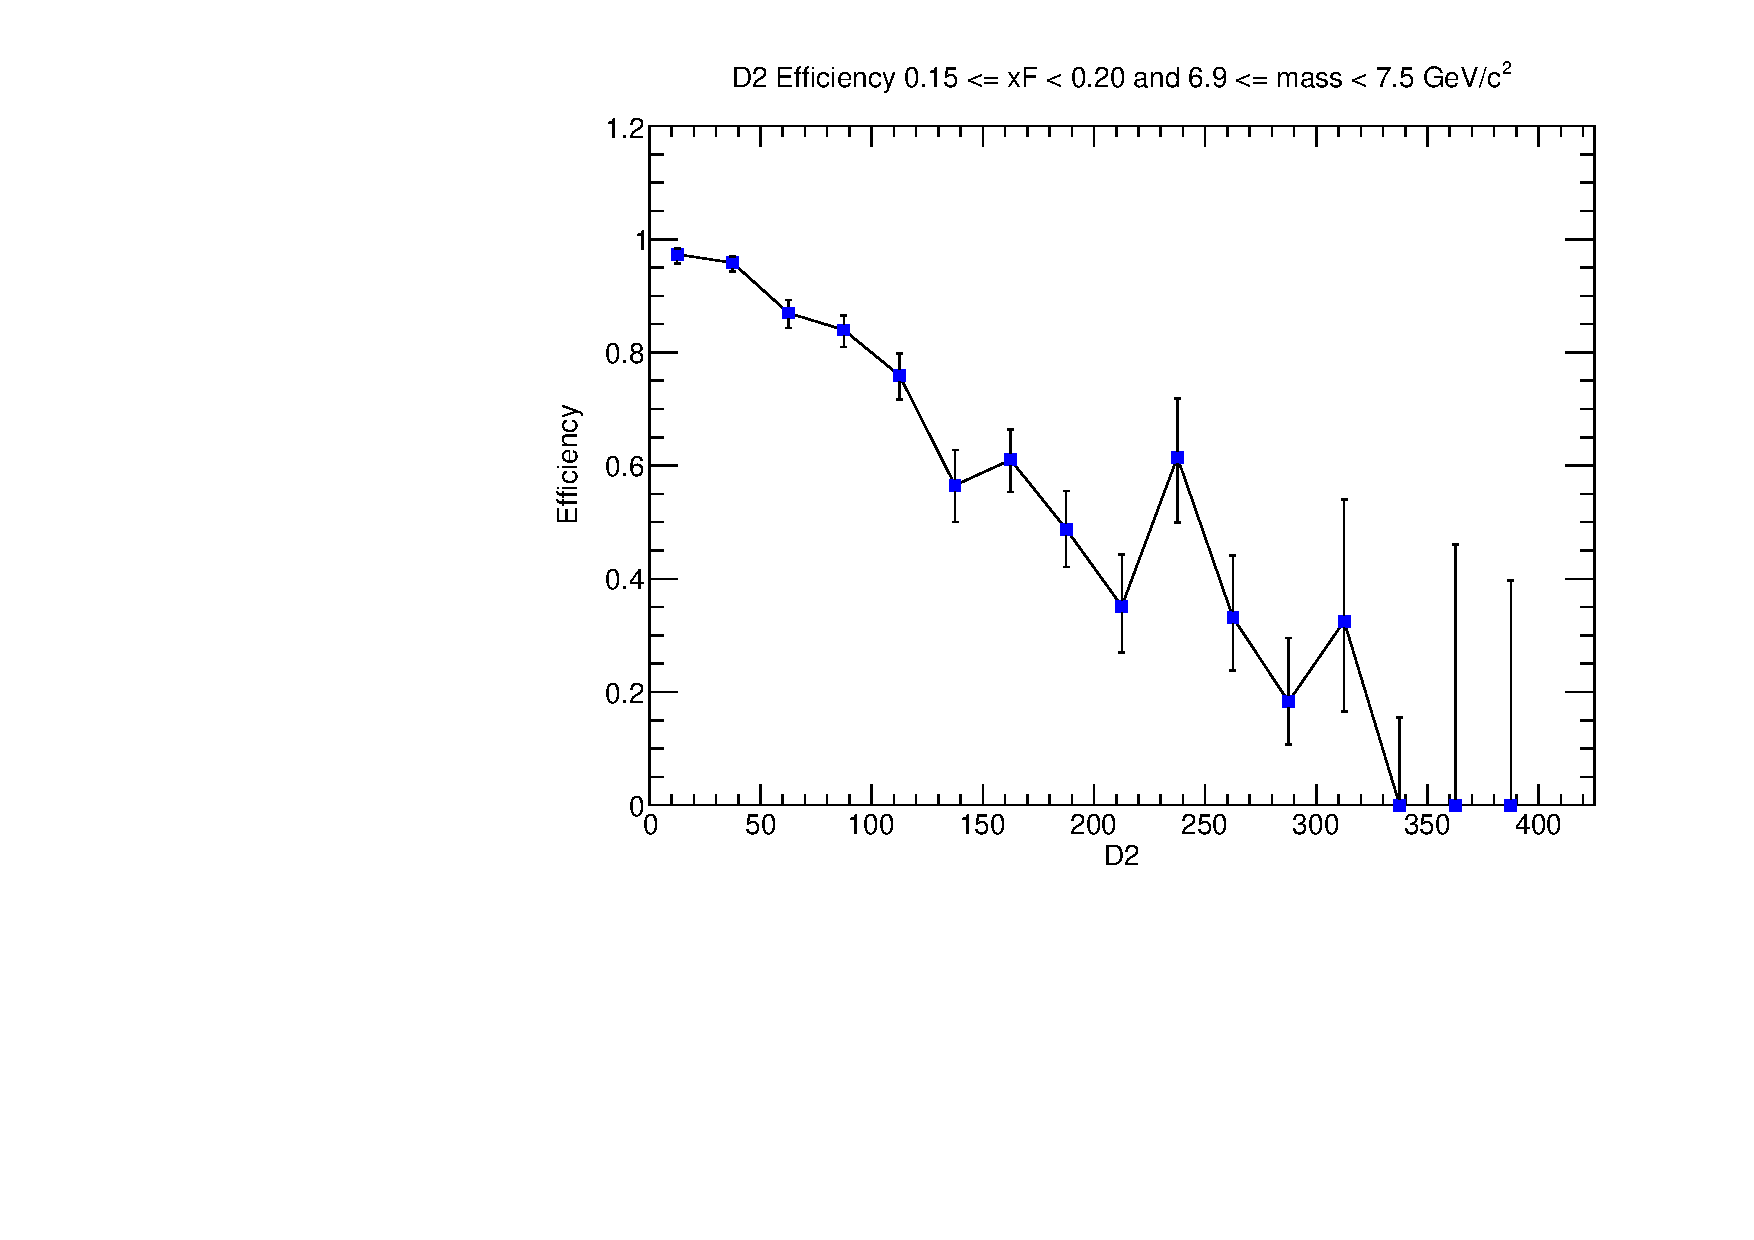
\includegraphics[width=\textwidth]{./kTrackerEfficiencyPlots/D2_Efficiency_xF3_mass9.pdf}
        \caption{$6.9 \leq m < 7.5$ GeV/$c^2$}
        \label{fig:xF3_mass9}
    \end{subfigure}
    \hfill
    \begin{subfigure}[b]{0.32\textwidth}
        \centering
        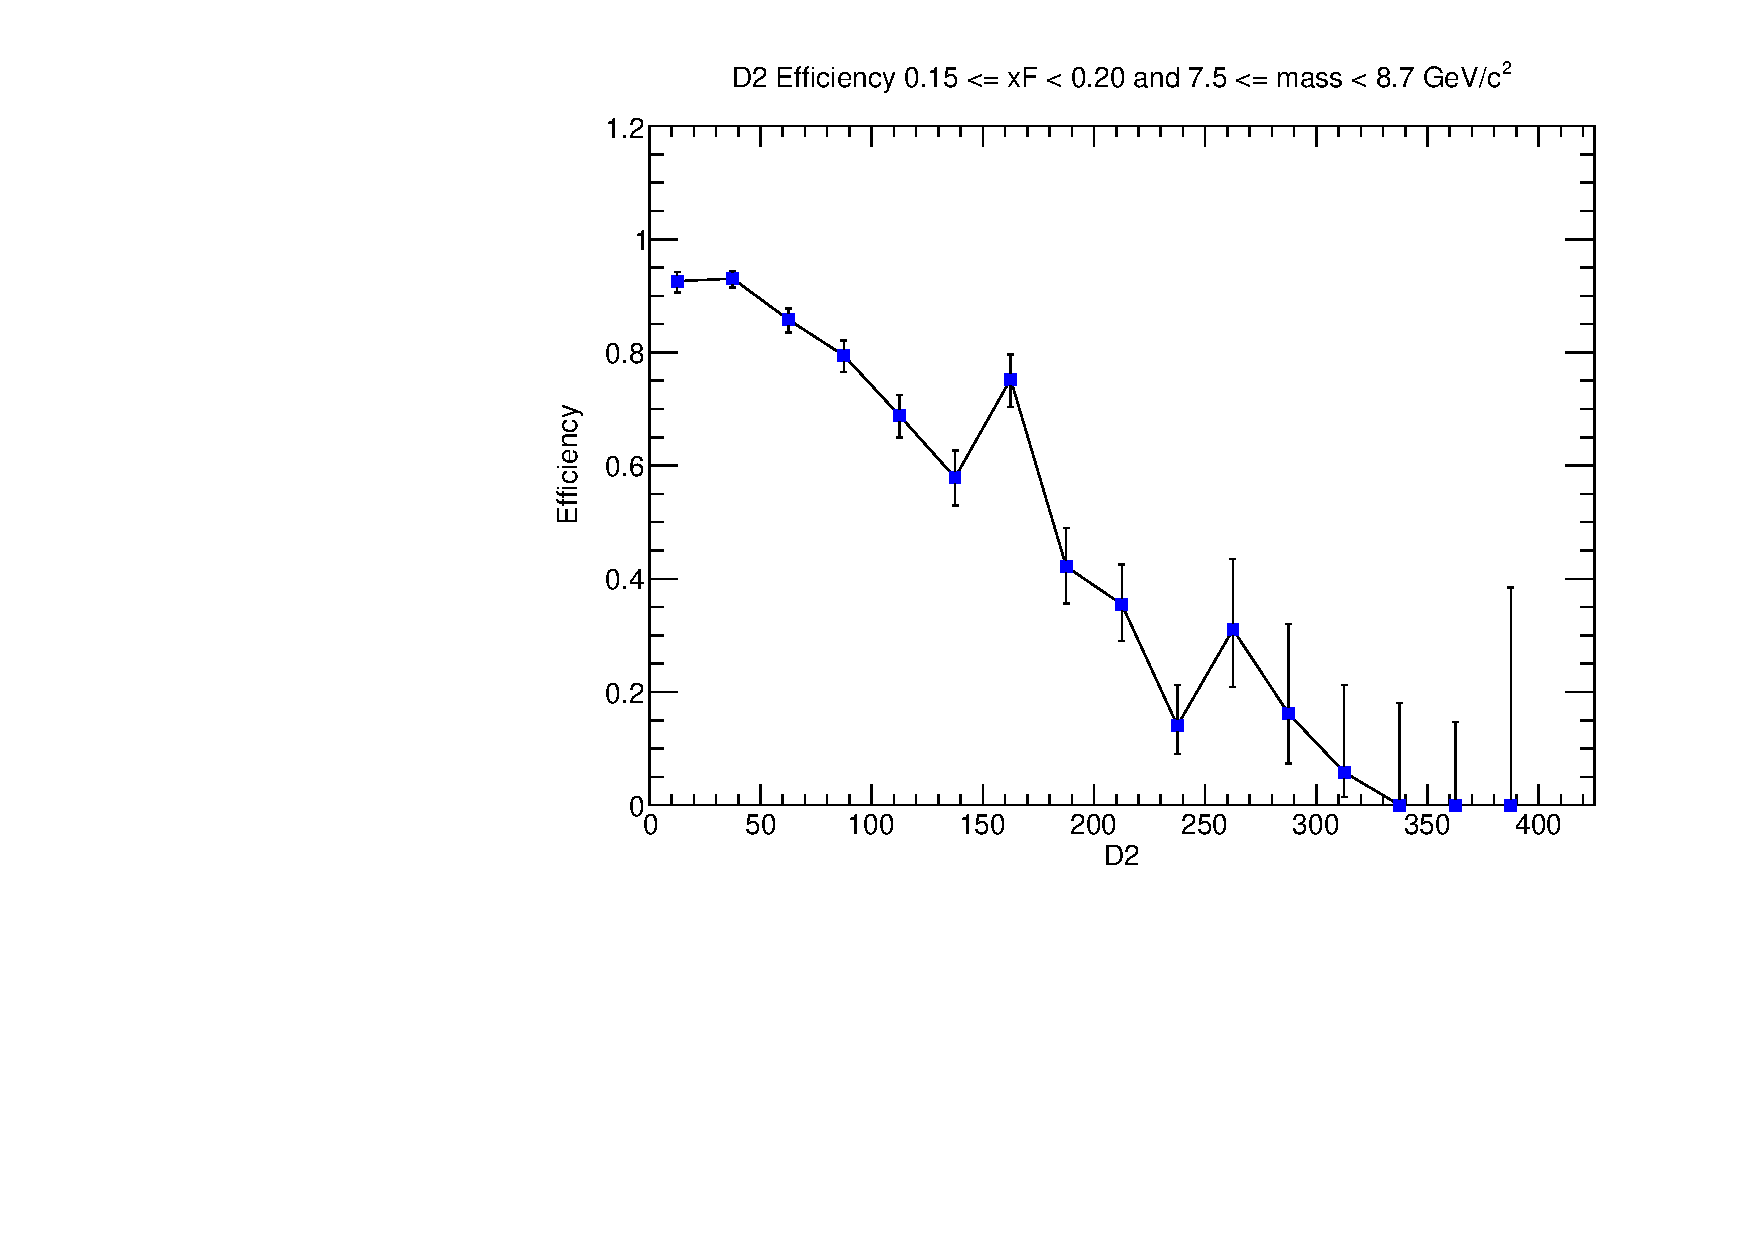
\includegraphics[width=\textwidth]{./kTrackerEfficiencyPlots/D2_Efficiency_xF3_mass10.pdf}
        \caption{$7.5 \leq m < 8.7$ GeV/$c^2$}
        \label{fig:xF3_mass10}
    \end{subfigure}
    \hfill
    \caption{Efficiency plots for the $x_F$ bin $0.15 \leq x_F < 0.20$.}
    \label{fig:xF3}
\end{figure}

\clearpage

\begin{figure}[p]
    \centering
    \begin{subfigure}[b]{0.32\textwidth}
        \centering
        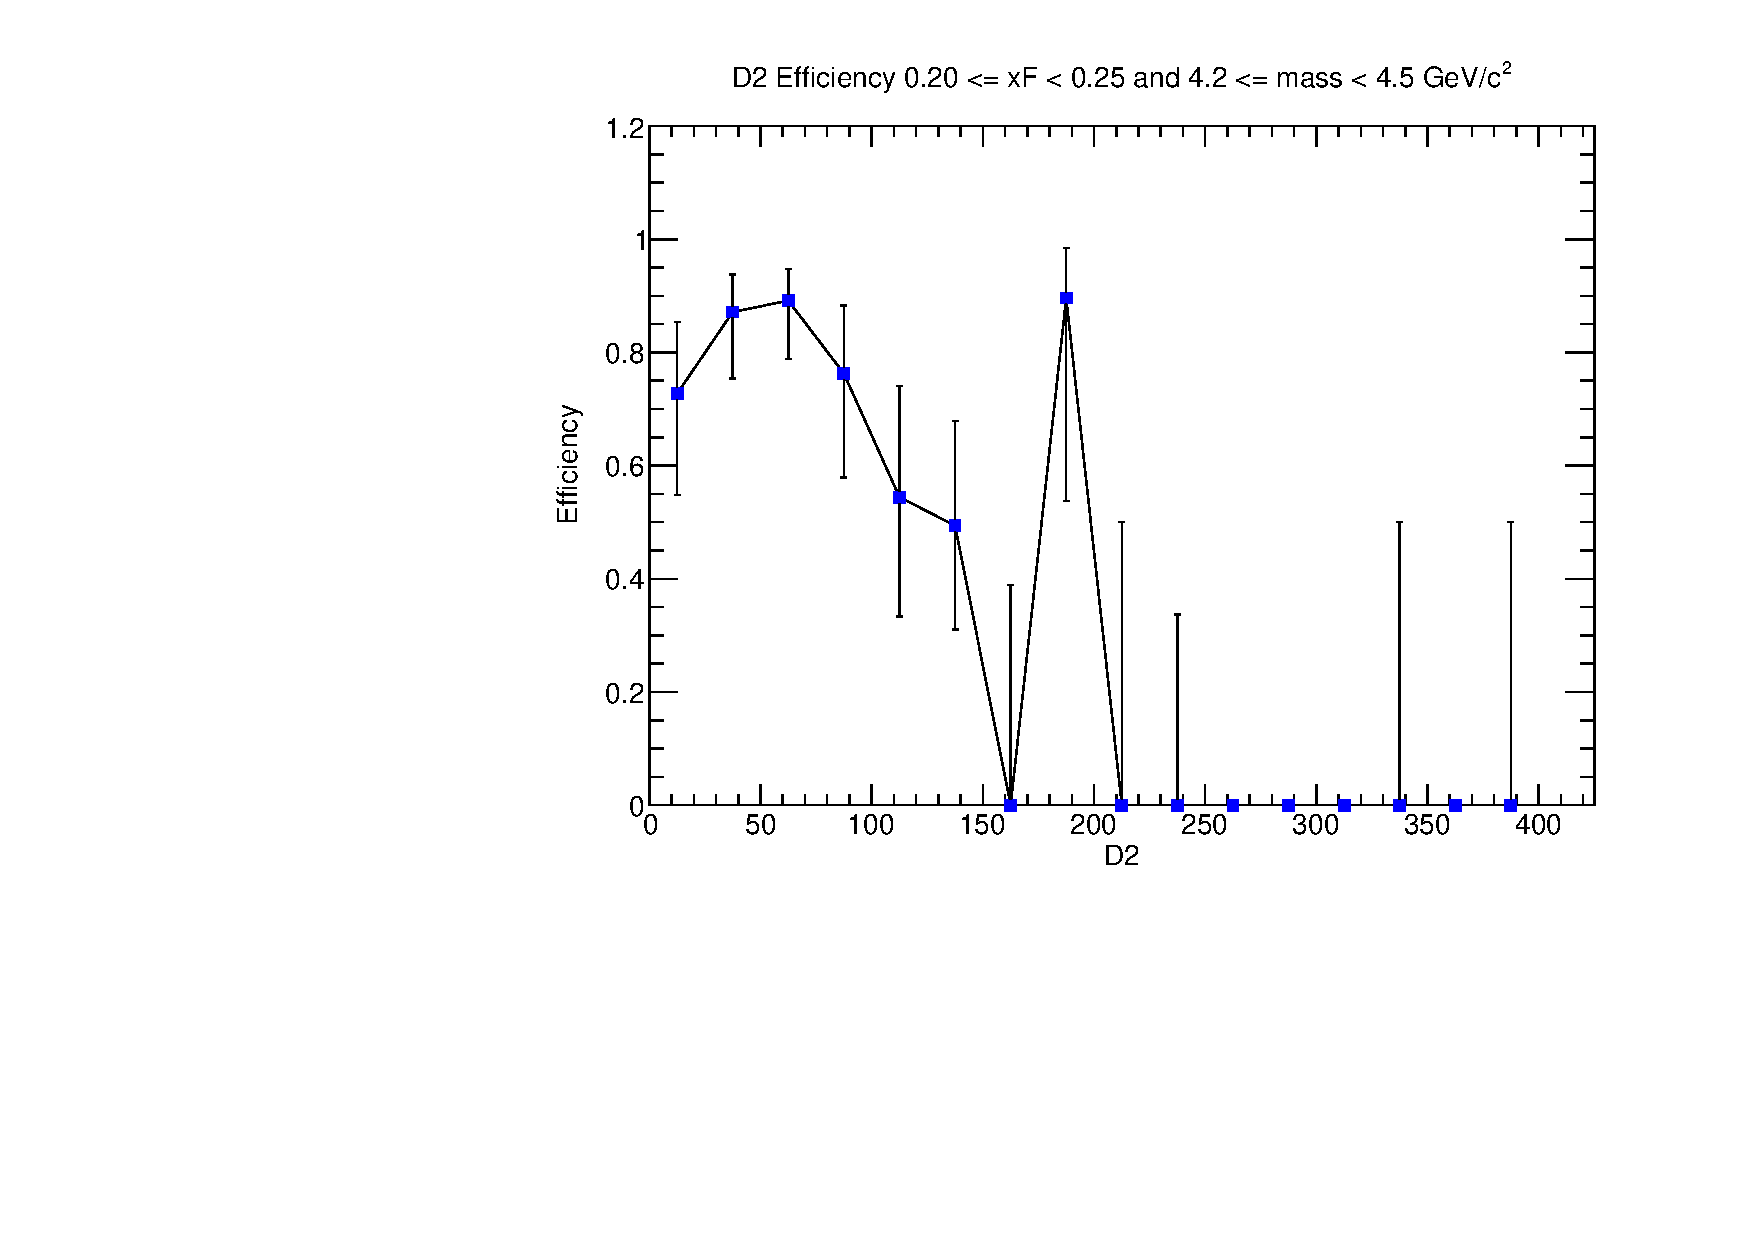
\includegraphics[width=\textwidth]{./kTrackerEfficiencyPlots/D2_Efficiency_xF4_mass0.pdf}
        \caption{$4.2 \leq m < 4.5$ GeV/$c^2$}
        \label{fig:xF4_mass0}
    \end{subfigure}
    \hfill
    \begin{subfigure}[b]{0.32\textwidth}
        \centering
        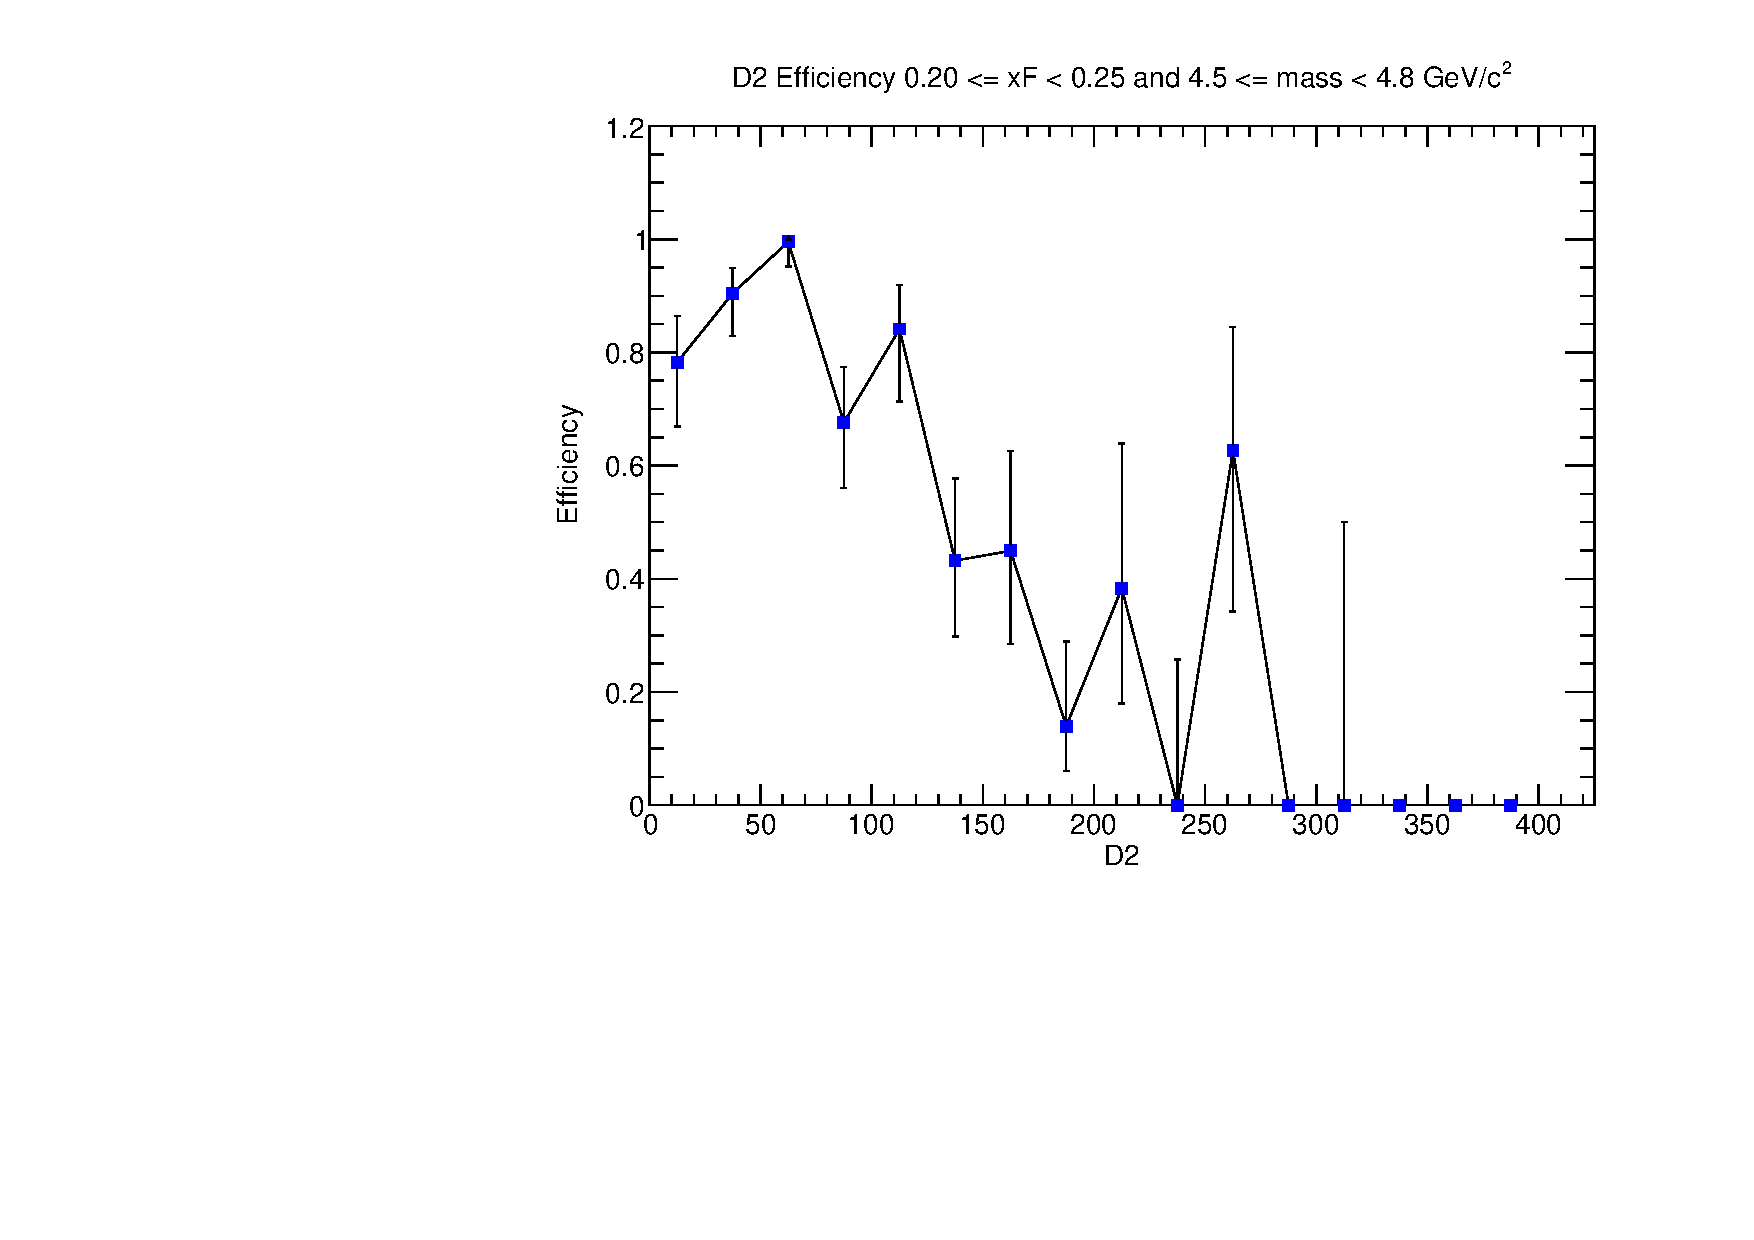
\includegraphics[width=\textwidth]{./kTrackerEfficiencyPlots/D2_Efficiency_xF4_mass1.pdf}
        \caption{$4.5 \leq m < 4.8$ GeV/$c^2$}
        \label{fig:xF4_mass1}
    \end{subfigure}
    \hfill
    \begin{subfigure}[b]{0.32\textwidth}
        \centering
        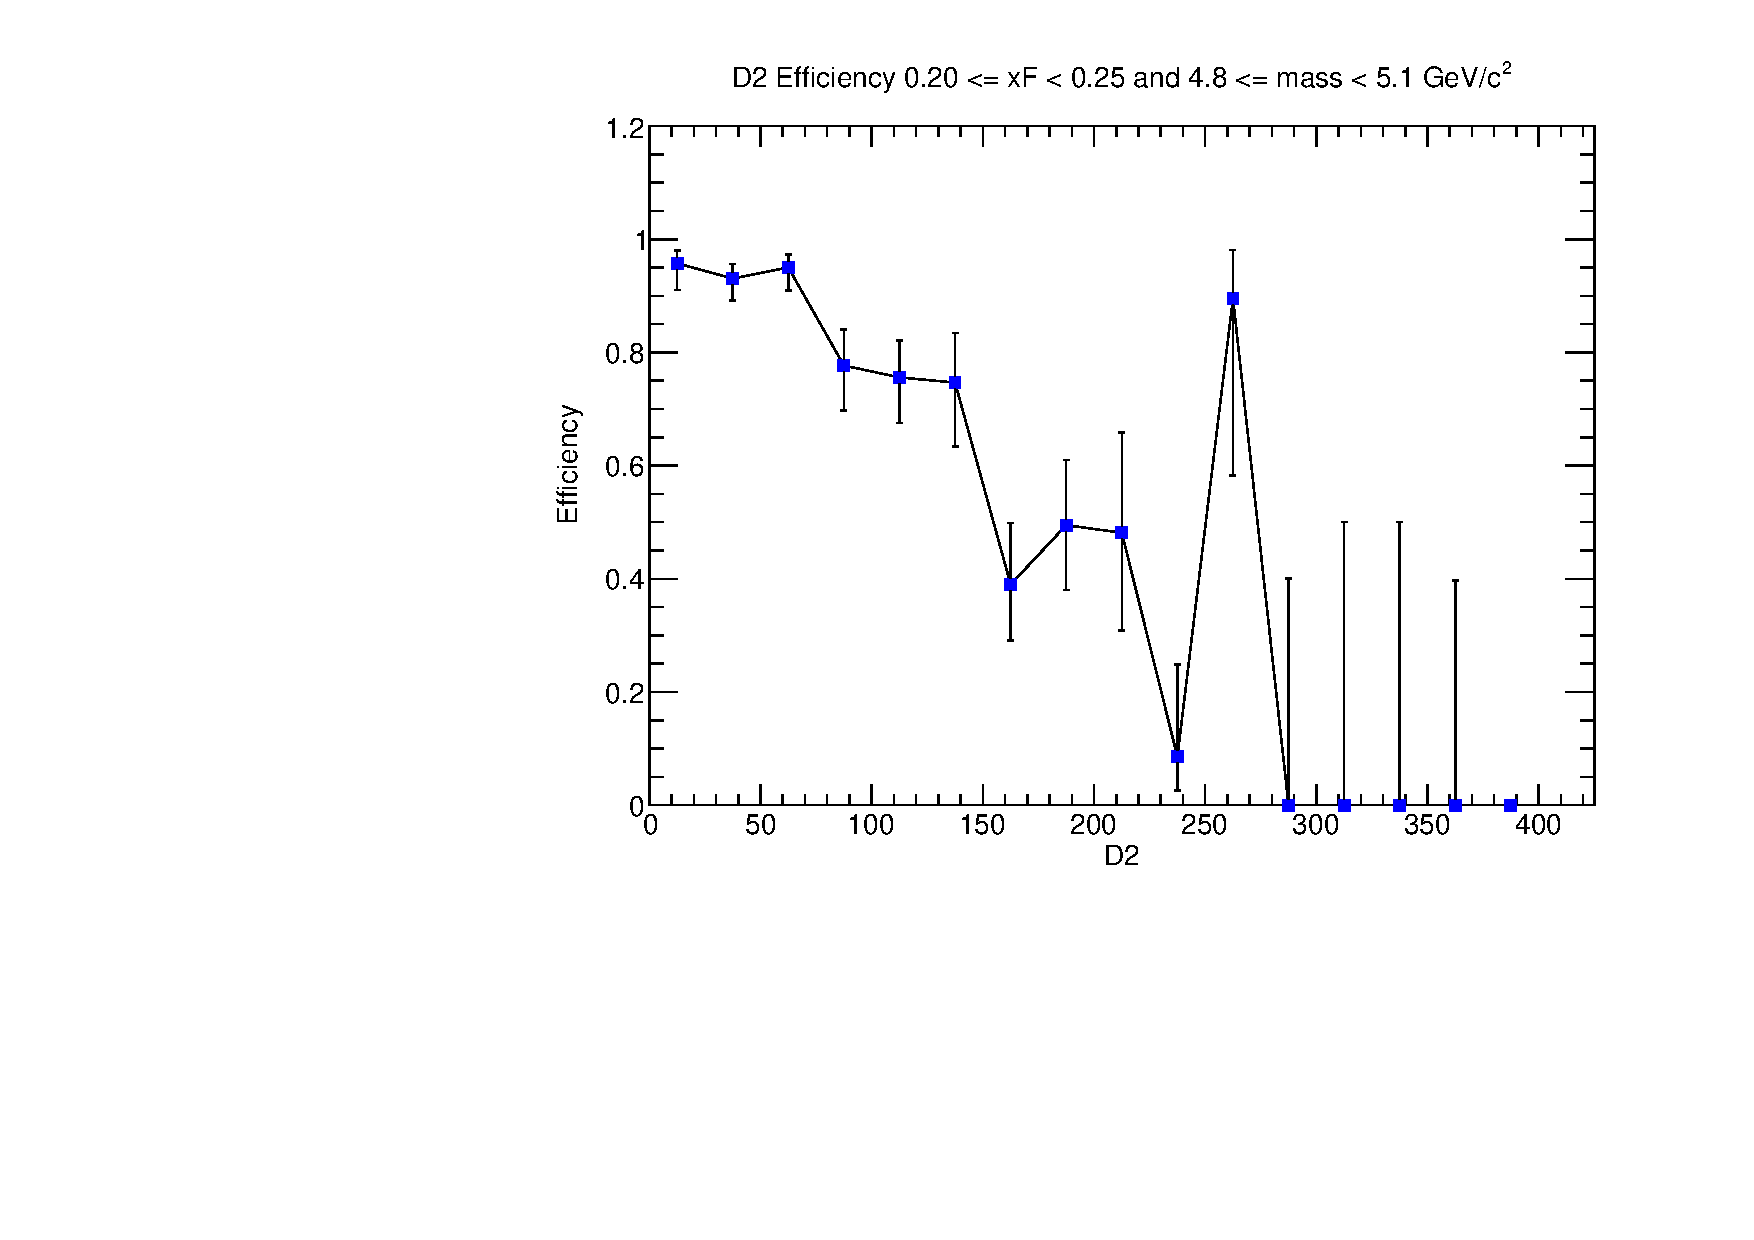
\includegraphics[width=\textwidth]{./kTrackerEfficiencyPlots/D2_Efficiency_xF4_mass2.pdf}
        \caption{$4.8 \leq m < 5.1$ GeV/$c^2$}
        \label{fig:xF4_mass2}
    \end{subfigure}
    \vspace{0.5cm}
    \begin{subfigure}[b]{0.32\textwidth}
        \centering
        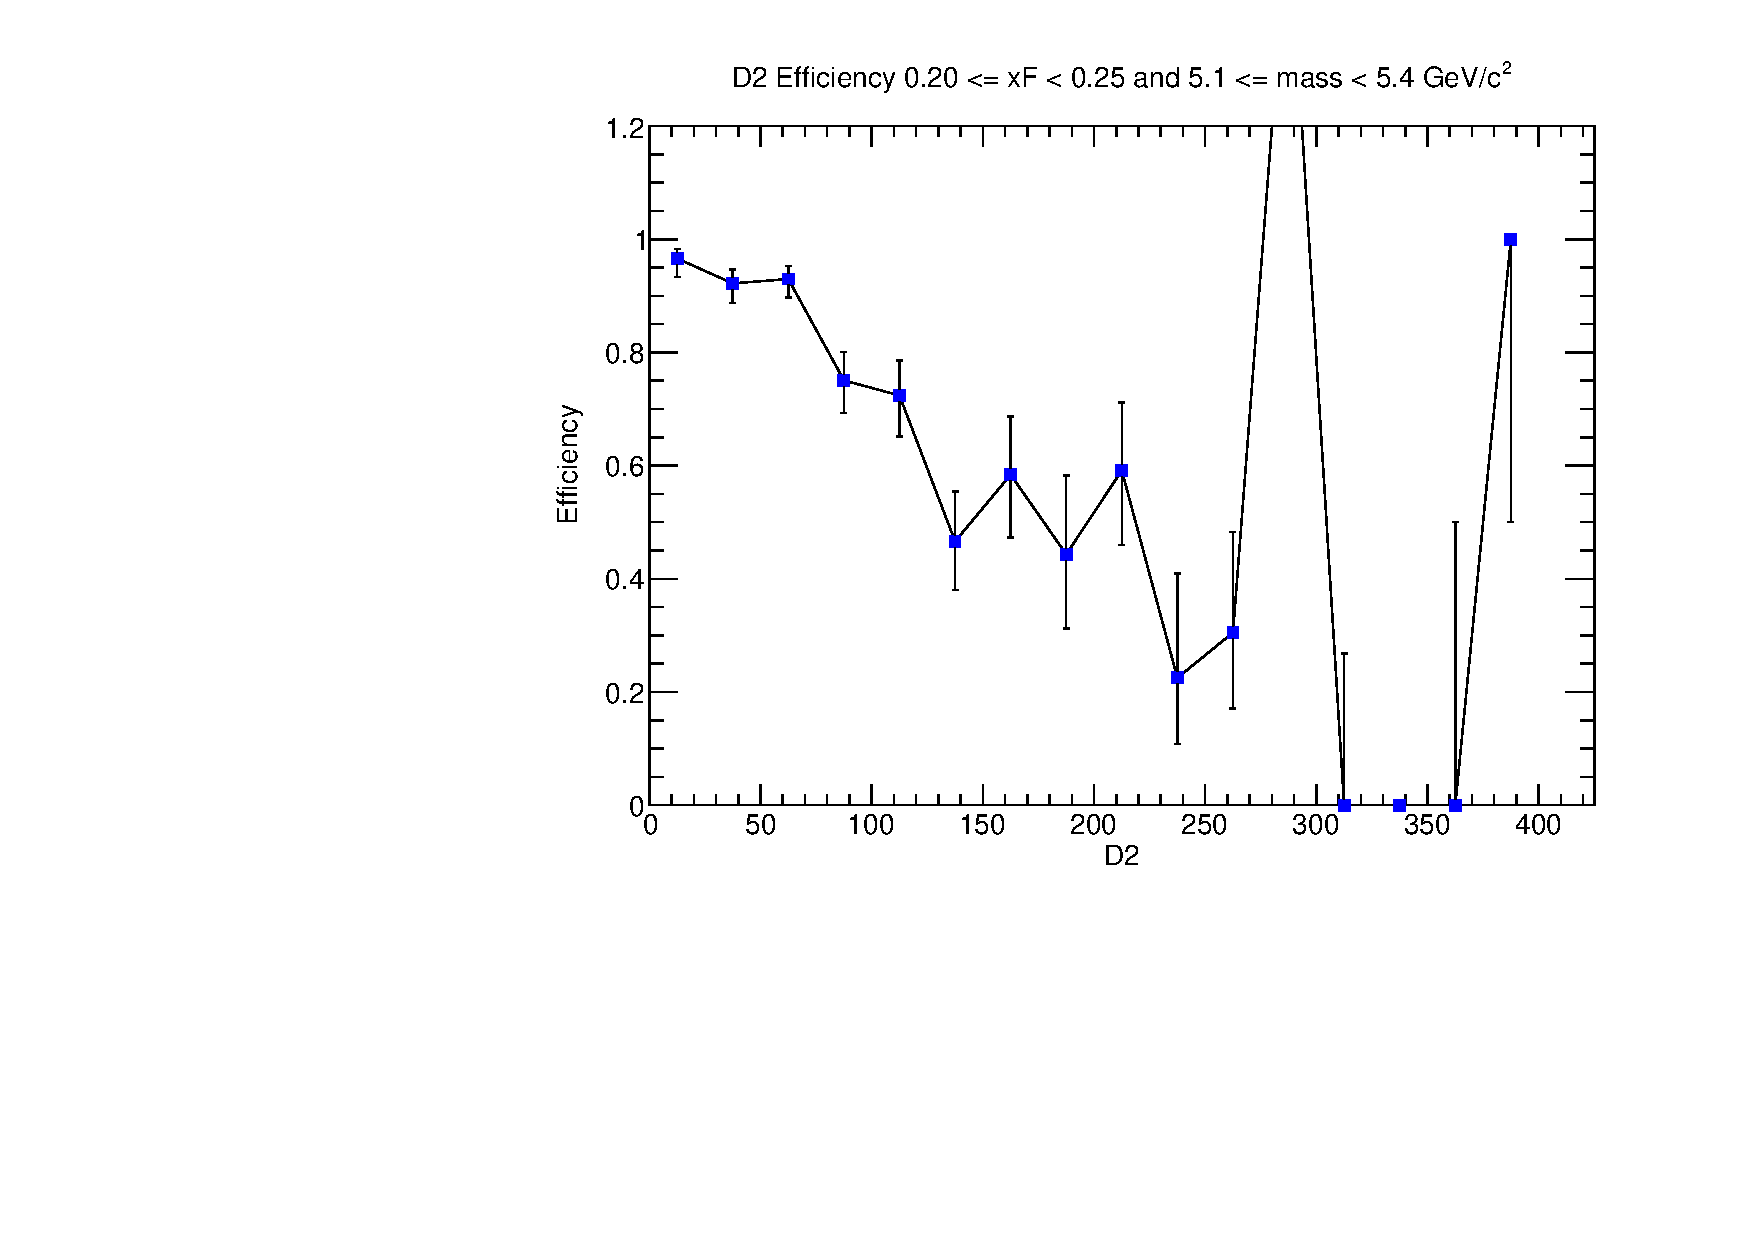
\includegraphics[width=\textwidth]{./kTrackerEfficiencyPlots/D2_Efficiency_xF4_mass3.pdf}
        \caption{$5.1 \leq m < 5.4$ GeV/$c^2$}
        \label{fig:xF4_mass3}
    \end{subfigure}
    \hfill
    \begin{subfigure}[b]{0.32\textwidth}
        \centering
        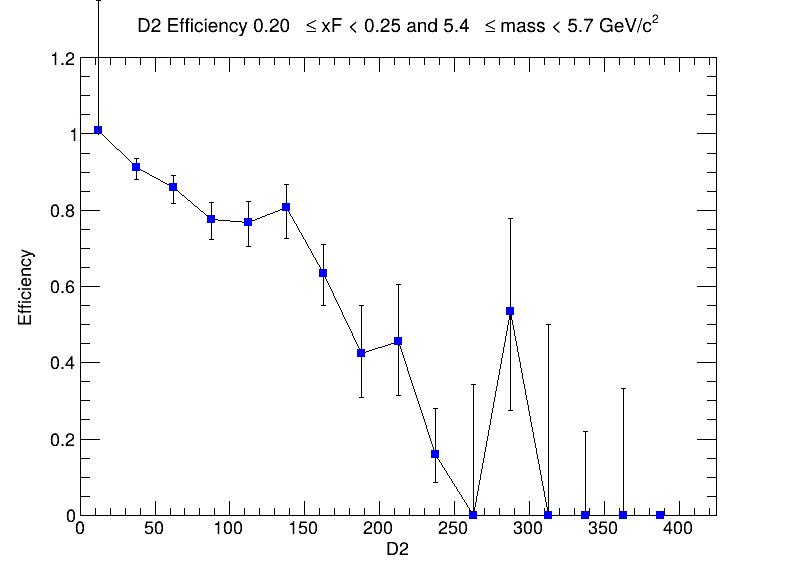
\includegraphics[width=\textwidth]{./kTrackerEfficiencyPlots/D2_Efficiency_xF4_mass4.png}
        \caption{$5.4 \leq m < 5.7$ GeV/$c^2$}
        \label{fig:xF4_mass4}
    \end{subfigure}
    \hfill
    \begin{subfigure}[b]{0.32\textwidth}
        \centering
        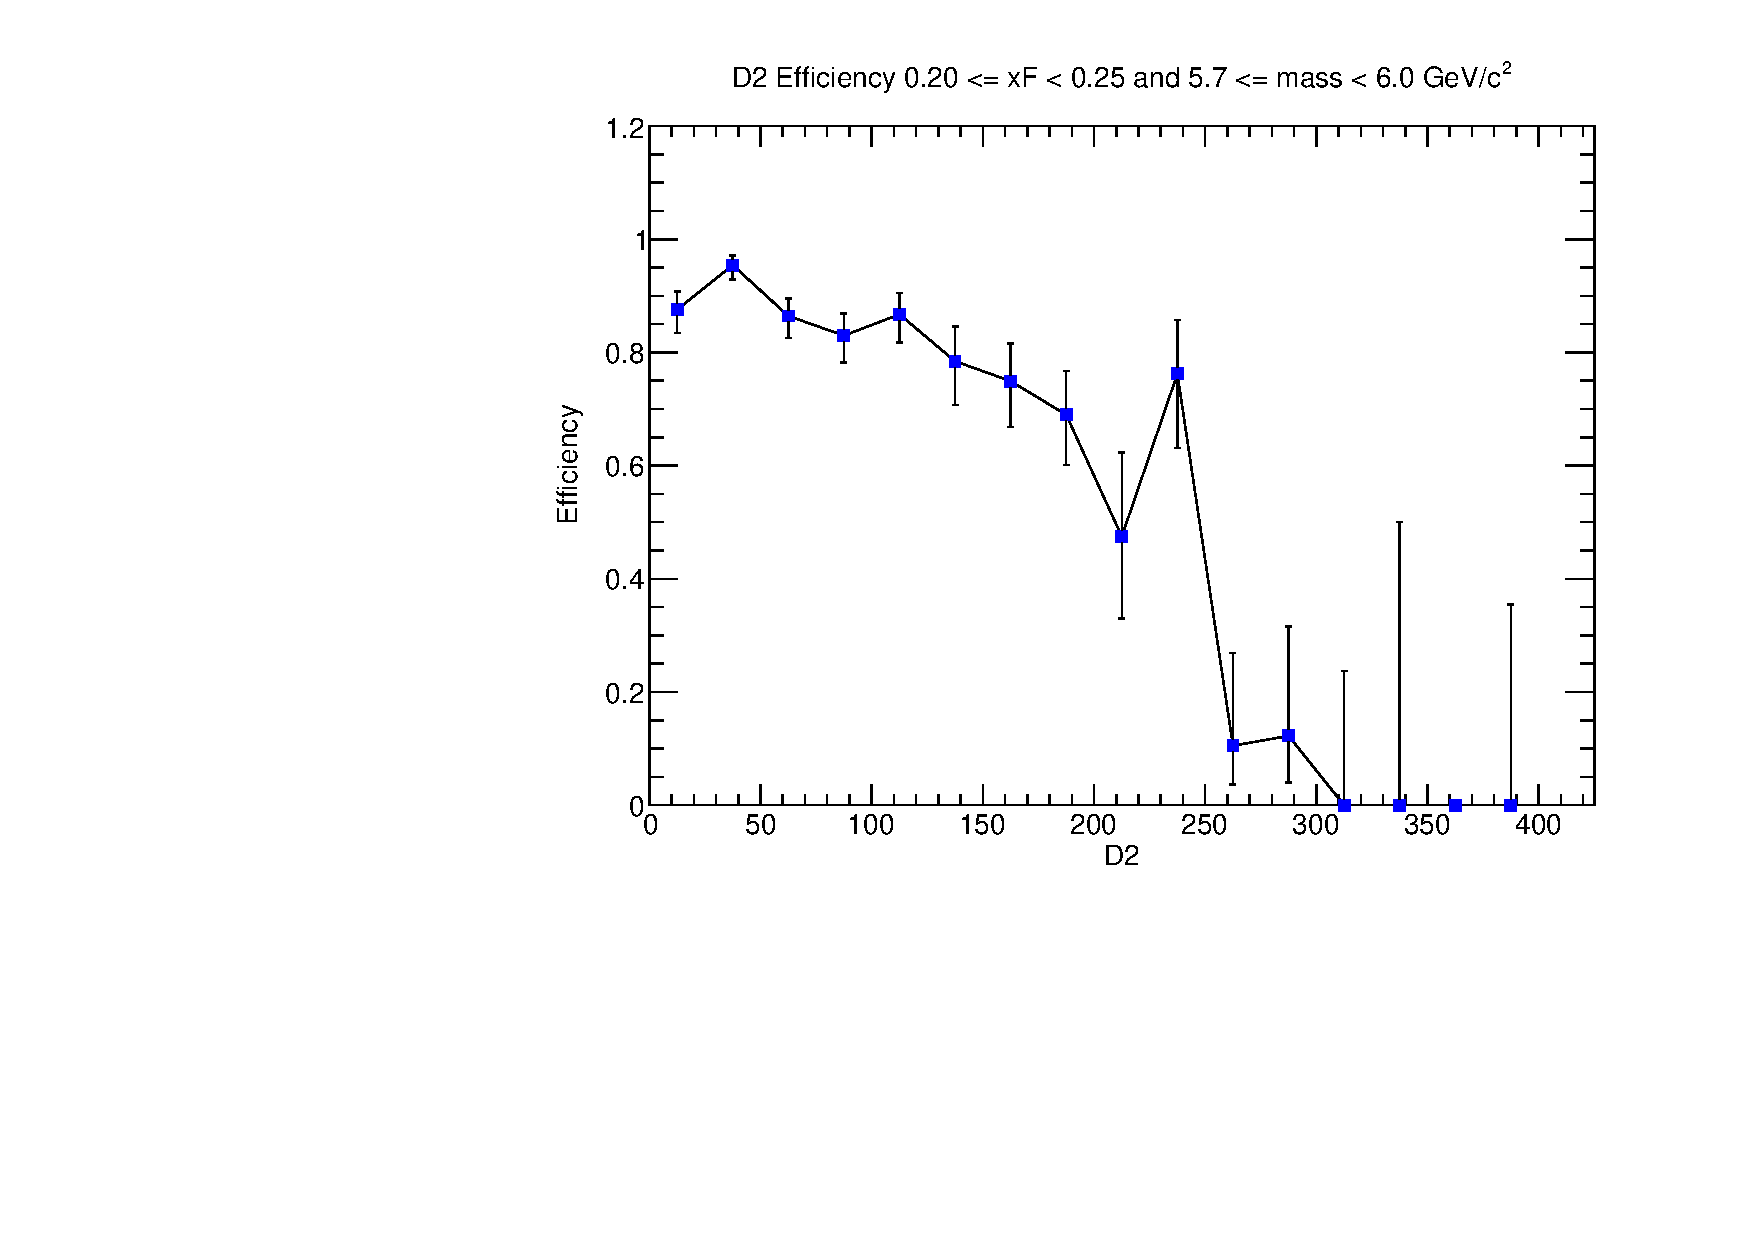
\includegraphics[width=\textwidth]{./kTrackerEfficiencyPlots/D2_Efficiency_xF4_mass5.pdf}
        \caption{$5.7 \leq m < 6.0$ GeV/$c^2$}
        \label{fig:xF4_mass5}
    \end{subfigure}
    \vspace{0.5cm}
    \begin{subfigure}[b]{0.32\textwidth}
        \centering
        \includegraphics[width=\textwidth]{./kTrackerEfficiencyPlots/D2_Efficiency_xF4_mass6.png}
        \caption{$6.0 \leq m < 6.3$ GeV/$c^2$}
        \label{fig:xF4_mass6}
    \end{subfigure}
    \hfill
    \begin{subfigure}[b]{0.32\textwidth}
        \centering
        \includegraphics[width=\textwidth]{./kTrackerEfficiencyPlots/D2_Efficiency_xF4_mass7.pdf}
        \caption{$6.3 \leq m < 6.6$ GeV/$c^2$}
        \label{fig:xF4_mass7}
    \end{subfigure}
    \hfill
    \begin{subfigure}[b]{0.32\textwidth}
        \centering
        \includegraphics[width=\textwidth]{./kTrackerEfficiencyPlots/D2_Efficiency_xF4_mass8.pdf}
        \caption{$6.6 \leq m < 6.9$ GeV/$c^2$}
        \label{fig:xF4_mass8}
    \end{subfigure}
    \vspace{0.5cm}
    \begin{subfigure}[b]{0.32\textwidth}
        \centering
        \includegraphics[width=\textwidth]{./kTrackerEfficiencyPlots/D2_Efficiency_xF4_mass9.png}
        \caption{$6.9 \leq m < 7.5$ GeV/$c^2$}
        \label{fig:xF4_mass9}
    \end{subfigure}
    \hfill
    \begin{subfigure}[b]{0.32\textwidth}
        \centering
        \includegraphics[width=\textwidth]{./kTrackerEfficiencyPlots/D2_Efficiency_xF4_mass10.pdf}
        \caption{$7.5 \leq m < 8.7$ GeV/$c^2$}
        \label{fig:xF4_mass10}
    \end{subfigure}
    \hfill
    \caption{Efficiency plots for the $x_F$ bin $0.20 \leq x_F < 0.25$.}
    \label{fig:xF4}
\end{figure}

\clearpage

\begin{figure}[p]
    \centering
    \begin{subfigure}[b]{0.32\textwidth}
        \centering
        \includegraphics[width=\textwidth]{./kTrackerEfficiencyPlots/D2_Efficiency_xF5_mass0.png}
        \caption{$4.2 \leq m < 4.5$ GeV/$c^2$}
        \label{fig:xF5_mass0}
    \end{subfigure}
    \hfill
    \begin{subfigure}[b]{0.32\textwidth}
        \centering
        \includegraphics[width=\textwidth]{./kTrackerEfficiencyPlots/D2_Efficiency_xF5_mass1.pdf}
        \caption{$4.5 \leq m < 4.8$ GeV/$c^2$}
        \label{fig:xF5_mass1}
    \end{subfigure}
    \hfill
    \begin{subfigure}[b]{0.32\textwidth}
        \centering
        \includegraphics[width=\textwidth]{./kTrackerEfficiencyPlots/D2_Efficiency_xF5_mass2.pdf}
        \caption{$4.8 \leq m < 5.1$ GeV/$c^2$}
        \label{fig:xF5_mass2}
    \end{subfigure}
    \vspace{0.5cm}
    \begin{subfigure}[b]{0.32\textwidth}
        \centering
        \includegraphics[width=\textwidth]{./kTrackerEfficiencyPlots/D2_Efficiency_xF5_mass3.pdf}
        \caption{$5.1 \leq m < 5.4$ GeV/$c^2$}
        \label{fig:xF5_mass3}
    \end{subfigure}
    \hfill
    \begin{subfigure}[b]{0.32\textwidth}
        \centering
        \includegraphics[width=\textwidth]{./kTrackerEfficiencyPlots/D2_Efficiency_xF5_mass4.png}
        \caption{$5.4 \leq m < 5.7$ GeV/$c^2$}
        \label{fig:xF5_mass4}
    \end{subfigure}
    \hfill
    \begin{subfigure}[b]{0.32\textwidth}
        \centering
        \includegraphics[width=\textwidth]{./kTrackerEfficiencyPlots/D2_Efficiency_xF5_mass5.png}
        \caption{$5.7 \leq m < 6.0$ GeV/$c^2$}
        \label{fig:xF5_mass5}
    \end{subfigure}
    \vspace{0.5cm}
    \begin{subfigure}[b]{0.32\textwidth}
        \centering
        \includegraphics[width=\textwidth]{./kTrackerEfficiencyPlots/D2_Efficiency_xF5_mass6.pdf}
        \caption{$6.0 \leq m < 6.3$ GeV/$c^2$}
        \label{fig:xF5_mass6}
    \end{subfigure}
    \hfill
    \begin{subfigure}[b]{0.32\textwidth}
        \centering
        \includegraphics[width=\textwidth]{./kTrackerEfficiencyPlots/D2_Efficiency_xF5_mass7.png}
        \caption{$6.3 \leq m < 6.6$ GeV/$c^2$}
        \label{fig:xF5_mass7}
    \end{subfigure}
    \hfill
    \begin{subfigure}[b]{0.32\textwidth}
        \centering
        \includegraphics[width=\textwidth]{./kTrackerEfficiencyPlots/D2_Efficiency_xF5_mass8.pdf}
        \caption{$6.6 \leq m < 6.9$ GeV/$c^2$}
        \label{fig:xF5_mass8}
    \end{subfigure}
    \vspace{0.5cm}
    \begin{subfigure}[b]{0.32\textwidth}
        \centering
        \includegraphics[width=\textwidth]{./kTrackerEfficiencyPlots/D2_Efficiency_xF5_mass9.pdf}
        \caption{$6.9 \leq m < 7.5$ GeV/$c^2$}
        \label{fig:xF5_mass9}
    \end{subfigure}
    \hfill
    \begin{subfigure}[b]{0.32\textwidth}
        \centering
        \includegraphics[width=\textwidth]{./kTrackerEfficiencyPlots/D2_Efficiency_xF5_mass10.pdf}
        \caption{$7.5 \leq m < 8.7$ GeV/$c^2$}
        \label{fig:xF5_mass10}
    \end{subfigure}
    \hfill
    \caption{Efficiency plots for the $x_F$ bin $0.25 \leq x_F < 0.30$.}
    \label{fig:xF5}
\end{figure}

\clearpage

\begin{figure}[p]
    \centering
    \begin{subfigure}[b]{0.32\textwidth}
        \centering
        \includegraphics[width=\textwidth]{./kTrackerEfficiencyPlots/D2_Efficiency_xF6_mass0.pdf}
        \caption{$4.2 \leq m < 4.5$ GeV/$c^2$}
        \label{fig:xF6_mass0}
    \end{subfigure}
    \hfill
    \begin{subfigure}[b]{0.32\textwidth}
        \centering
        \includegraphics[width=\textwidth]{./kTrackerEfficiencyPlots/D2_Efficiency_xF6_mass1.pdf}
        \caption{$4.5 \leq m < 4.8$ GeV/$c^2$}
        \label{fig:xF6_mass1}
    \end{subfigure}
    \hfill
    \begin{subfigure}[b]{0.32\textwidth}
        \centering
        \includegraphics[width=\textwidth]{./kTrackerEfficiencyPlots/D2_Efficiency_xF6_mass2.pdf}
        \caption{$4.8 \leq m < 5.1$ GeV/$c^2$}
        \label{fig:xF6_mass2}
    \end{subfigure}
    \vspace{0.5cm}
    \begin{subfigure}[b]{0.32\textwidth}
        \centering
        \includegraphics[width=\textwidth]{./kTrackerEfficiencyPlots/D2_Efficiency_xF6_mass3.png}
        \caption{$5.1 \leq m < 5.4$ GeV/$c^2$}
        \label{fig:xF6_mass3}
    \end{subfigure}
    \hfill
    \begin{subfigure}[b]{0.32\textwidth}
        \centering
        \includegraphics[width=\textwidth]{./kTrackerEfficiencyPlots/D2_Efficiency_xF6_mass4.png}
        \caption{$5.4 \leq m < 5.7$ GeV/$c^2$}
        \label{fig:xF6_mass4}
    \end{subfigure}
    \hfill
    \begin{subfigure}[b]{0.32\textwidth}
        \centering
        \includegraphics[width=\textwidth]{./kTrackerEfficiencyPlots/D2_Efficiency_xF6_mass5.pdf}
        \caption{$5.7 \leq m < 6.0$ GeV/$c^2$}
        \label{fig:xF6_mass5}
    \end{subfigure}
    \vspace{0.5cm}
    \begin{subfigure}[b]{0.32\textwidth}
        \centering
        \includegraphics[width=\textwidth]{./kTrackerEfficiencyPlots/D2_Efficiency_xF6_mass6.png}
        \caption{$6.0 \leq m < 6.3$ GeV/$c^2$}
        \label{fig:xF6_mass6}
    \end{subfigure}
    \hfill
    \begin{subfigure}[b]{0.32\textwidth}
        \centering
        \includegraphics[width=\textwidth]{./kTrackerEfficiencyPlots/D2_Efficiency_xF6_mass7.pdf}
        \caption{$6.3 \leq m < 6.6$ GeV/$c^2$}
        \label{fig:xF6_mass7}
    \end{subfigure}
    \hfill
    \begin{subfigure}[b]{0.32\textwidth}
        \centering
        \includegraphics[width=\textwidth]{./kTrackerEfficiencyPlots/D2_Efficiency_xF6_mass8.pdf}
        \caption{$6.6 \leq m < 6.9$ GeV/$c^2$}
        \label{fig:xF6_mass8}
    \end{subfigure}
    \vspace{0.5cm}
    \begin{subfigure}[b]{0.32\textwidth}
        \centering
        \includegraphics[width=\textwidth]{./kTrackerEfficiencyPlots/D2_Efficiency_xF6_mass9.pdf}
        \caption{$6.9 \leq m < 7.5$ GeV/$c^2$}
        \label{fig:xF6_mass9}
    \end{subfigure}
    \hfill
    \begin{subfigure}[b]{0.32\textwidth}
        \centering
        \includegraphics[width=\textwidth]{./kTrackerEfficiencyPlots/D2_Efficiency_xF6_mass10.pdf}
        \caption{$7.5 \leq m < 8.7$ GeV/$c^2$}
        \label{fig:xF6_mass10}
    \end{subfigure}
    \hfill
    \caption{Efficiency plots for the $x_F$ bin $0.30 \leq x_F < 0.35$.}
    \label{fig:xF6}
\end{figure}

\clearpage

\begin{figure}[p]
    \centering
    \begin{subfigure}[b]{0.32\textwidth}
        \centering
        \includegraphics[width=\textwidth]{./kTrackerEfficiencyPlots/D2_Efficiency_xF7_mass0.pdf}
        \caption{$4.2 \leq m < 4.5$ GeV/$c^2$}
        \label{fig:xF7_mass0}
    \end{subfigure}
    \hfill
    \begin{subfigure}[b]{0.32\textwidth}
        \centering
        \includegraphics[width=\textwidth]{./kTrackerEfficiencyPlots/D2_Efficiency_xF7_mass1.pdf}
        \caption{$4.5 \leq m < 4.8$ GeV/$c^2$}
        \label{fig:xF7_mass1}
    \end{subfigure}
    \hfill
    \begin{subfigure}[b]{0.32\textwidth}
        \centering
        \includegraphics[width=\textwidth]{./kTrackerEfficiencyPlots/D2_Efficiency_xF7_mass2.png}
        \caption{$4.8 \leq m < 5.1$ GeV/$c^2$}
        \label{fig:xF7_mass2}
    \end{subfigure}
    \vspace{0.5cm}
    \begin{subfigure}[b]{0.32\textwidth}
        \centering
        \includegraphics[width=\textwidth]{./kTrackerEfficiencyPlots/D2_Efficiency_xF7_mass3.pdf}
        \caption{$5.1 \leq m < 5.4$ GeV/$c^2$}
        \label{fig:xF7_mass3}
    \end{subfigure}
    \hfill
    \begin{subfigure}[b]{0.32\textwidth}
        \centering
        \includegraphics[width=\textwidth]{./kTrackerEfficiencyPlots/D2_Efficiency_xF7_mass4.png}
        \caption{$5.4 \leq m < 5.7$ GeV/$c^2$}
        \label{fig:xF7_mass4}
    \end{subfigure}
    \hfill
    \begin{subfigure}[b]{0.32\textwidth}
        \centering
        \includegraphics[width=\textwidth]{./kTrackerEfficiencyPlots/D2_Efficiency_xF7_mass5.pdf}
        \caption{$5.7 \leq m < 6.0$ GeV/$c^2$}
        \label{fig:xF7_mass5}
    \end{subfigure}
    \vspace{0.5cm}
    \begin{subfigure}[b]{0.32\textwidth}
        \centering
        \includegraphics[width=\textwidth]{./kTrackerEfficiencyPlots/D2_Efficiency_xF7_mass6.pdf}
        \caption{$6.0 \leq m < 6.3$ GeV/$c^2$}
        \label{fig:xF7_mass6}
    \end{subfigure}
    \hfill
    \begin{subfigure}[b]{0.32\textwidth}
        \centering
        \includegraphics[width=\textwidth]{./kTrackerEfficiencyPlots/D2_Efficiency_xF7_mass7.pdf}
        \caption{$6.3 \leq m < 6.6$ GeV/$c^2$}
        \label{fig:xF7_mass7}
    \end{subfigure}
    \hfill
    \begin{subfigure}[b]{0.32\textwidth}
        \centering
        \includegraphics[width=\textwidth]{./kTrackerEfficiencyPlots/D2_Efficiency_xF7_mass8.png}
        \caption{$6.6 \leq m < 6.9$ GeV/$c^2$}
        \label{fig:xF7_mass8}
    \end{subfigure}
    \vspace{0.5cm}
    \begin{subfigure}[b]{0.32\textwidth}
        \centering
        \includegraphics[width=\textwidth]{./kTrackerEfficiencyPlots/D2_Efficiency_xF7_mass9.pdf}
        \caption{$6.9 \leq m < 7.5$ GeV/$c^2$}
        \label{fig:xF7_mass9}
    \end{subfigure}
    \hfill
    \begin{subfigure}[b]{0.32\textwidth}
        \centering
        \includegraphics[width=\textwidth]{./kTrackerEfficiencyPlots/D2_Efficiency_xF7_mass10.pdf}
        \caption{$7.5 \leq m < 8.7$ GeV/$c^2$}
        \label{fig:xF7_mass10}
    \end{subfigure}
    \hfill
    \caption{Efficiency plots for the $x_F$ bin $0.35 \leq x_F < 0.40$.}
    \label{fig:xF7}
\end{figure}

\clearpage

\begin{figure}[p]
    \centering
    \begin{subfigure}[b]{0.32\textwidth}
        \centering
        \includegraphics[width=\textwidth]{./kTrackerEfficiencyPlots/D2_Efficiency_xF8_mass0.pdf}
        \caption{$4.2 \leq m < 4.5$ GeV/$c^2$}
        \label{fig:xF8_mass0}
    \end{subfigure}
    \hfill
    \begin{subfigure}[b]{0.32\textwidth}
        \centering
        \includegraphics[width=\textwidth]{./kTrackerEfficiencyPlots/D2_Efficiency_xF8_mass1.png}
        \caption{$4.5 \leq m < 4.8$ GeV/$c^2$}
        \label{fig:xF8_mass1}
    \end{subfigure}
    \hfill
    \begin{subfigure}[b]{0.32\textwidth}
        \centering
        \includegraphics[width=\textwidth]{./kTrackerEfficiencyPlots/D2_Efficiency_xF8_mass2.png}
        \caption{$4.8 \leq m < 5.1$ GeV/$c^2$}
        \label{fig:xF8_mass2}
    \end{subfigure}
    \vspace{0.5cm}
    \begin{subfigure}[b]{0.32\textwidth}
        \centering
        \includegraphics[width=\textwidth]{./kTrackerEfficiencyPlots/D2_Efficiency_xF8_mass3.png}
        \caption{$5.1 \leq m < 5.4$ GeV/$c^2$}
        \label{fig:xF8_mass3}
    \end{subfigure}
    \hfill
    \begin{subfigure}[b]{0.32\textwidth}
        \centering
        \includegraphics[width=\textwidth]{./kTrackerEfficiencyPlots/D2_Efficiency_xF8_mass4.pdf}
        \caption{$5.4 \leq m < 5.7$ GeV/$c^2$}
        \label{fig:xF8_mass4}
    \end{subfigure}
    \hfill
    \begin{subfigure}[b]{0.32\textwidth}
        \centering
        \includegraphics[width=\textwidth]{./kTrackerEfficiencyPlots/D2_Efficiency_xF8_mass5.pdf}
        \caption{$5.7 \leq m < 6.0$ GeV/$c^2$}
        \label{fig:xF8_mass5}
    \end{subfigure}
    \vspace{0.5cm}
    \begin{subfigure}[b]{0.32\textwidth}
        \centering
        \includegraphics[width=\textwidth]{./kTrackerEfficiencyPlots/D2_Efficiency_xF8_mass6.pdf}
        \caption{$6.0 \leq m < 6.3$ GeV/$c^2$}
        \label{fig:xF8_mass6}
    \end{subfigure}
    \hfill
    \begin{subfigure}[b]{0.32\textwidth}
        \centering
        \includegraphics[width=\textwidth]{./kTrackerEfficiencyPlots/D2_Efficiency_xF8_mass7.pdf}
        \caption{$6.3 \leq m < 6.6$ GeV/$c^2$}
        \label{fig:xF8_mass7}
    \end{subfigure}
    \hfill
    \begin{subfigure}[b]{0.32\textwidth}
        \centering
        \includegraphics[width=\textwidth]{./kTrackerEfficiencyPlots/D2_Efficiency_xF8_mass8.png}
        \caption{$6.6 \leq m < 6.9$ GeV/$c^2$}
        \label{fig:xF8_mass8}
    \end{subfigure}
    \vspace{0.5cm}
    \begin{subfigure}[b]{0.32\textwidth}
        \centering
        \includegraphics[width=\textwidth]{./kTrackerEfficiencyPlots/D2_Efficiency_xF8_mass9.pdf}
        \caption{$6.9 \leq m < 7.5$ GeV/$c^2$}
        \label{fig:xF8_mass9}
    \end{subfigure}
    \hfill
    \begin{subfigure}[b]{0.32\textwidth}
        \centering
        \includegraphics[width=\textwidth]{./kTrackerEfficiencyPlots/D2_Efficiency_xF8_mass10.pdf}
        \caption{$7.5 \leq m < 8.7$ GeV/$c^2$}
        \label{fig:xF8_mass10}
    \end{subfigure}
    \hfill
    \caption{Efficiency plots for the $x_F$ bin $0.40 \leq x_F < 0.45$.}
    \label{fig:xF8}
\end{figure}

\clearpage

\begin{figure}[p]
    \centering
    \begin{subfigure}[b]{0.32\textwidth}
        \centering
        \includegraphics[width=\textwidth]{./kTrackerEfficiencyPlots/D2_Efficiency_xF9_mass0.png}
        \caption{$4.2 \leq m < 4.5$ GeV/$c^2$}
        \label{fig:xF9_mass0}
    \end{subfigure}
    \hfill
    \begin{subfigure}[b]{0.32\textwidth}
        \centering
        \includegraphics[width=\textwidth]{./kTrackerEfficiencyPlots/D2_Efficiency_xF9_mass1.png}
        \caption{$4.5 \leq m < 4.8$ GeV/$c^2$}
        \label{fig:xF9_mass1}
    \end{subfigure}
    \hfill
    \begin{subfigure}[b]{0.32\textwidth}
        \centering
        \includegraphics[width=\textwidth]{./kTrackerEfficiencyPlots/D2_Efficiency_xF9_mass2.pdf}
        \caption{$4.8 \leq m < 5.1$ GeV/$c^2$}
        \label{fig:xF9_mass2}
    \end{subfigure}
    \vspace{0.5cm}
    \begin{subfigure}[b]{0.32\textwidth}
        \centering
        \includegraphics[width=\textwidth]{./kTrackerEfficiencyPlots/D2_Efficiency_xF9_mass3.pdf}
        \caption{$5.1 \leq m < 5.4$ GeV/$c^2$}
        \label{fig:xF9_mass3}
    \end{subfigure}
    \hfill
    \begin{subfigure}[b]{0.32\textwidth}
        \centering
        \includegraphics[width=\textwidth]{./kTrackerEfficiencyPlots/D2_Efficiency_xF9_mass4.pdf}
        \caption{$5.4 \leq m < 5.7$ GeV/$c^2$}
        \label{fig:xF9_mass4}
    \end{subfigure}
    \hfill
    \begin{subfigure}[b]{0.32\textwidth}
        \centering
        \includegraphics[width=\textwidth]{./kTrackerEfficiencyPlots/D2_Efficiency_xF9_mass5.png}
        \caption{$5.7 \leq m < 6.0$ GeV/$c^2$}
        \label{fig:xF9_mass5}
    \end{subfigure}
    \vspace{0.5cm}
    \begin{subfigure}[b]{0.32\textwidth}
        \centering
        \includegraphics[width=\textwidth]{./kTrackerEfficiencyPlots/D2_Efficiency_xF9_mass6.pdf}
        \caption{$6.0 \leq m < 6.3$ GeV/$c^2$}
        \label{fig:xF9_mass6}
    \end{subfigure}
    \hfill
    \begin{subfigure}[b]{0.32\textwidth}
        \centering
        \includegraphics[width=\textwidth]{./kTrackerEfficiencyPlots/D2_Efficiency_xF9_mass7.pdf}
        \caption{$6.3 \leq m < 6.6$ GeV/$c^2$}
        \label{fig:xF9_mass7}
    \end{subfigure}
    \hfill
    \begin{subfigure}[b]{0.32\textwidth}
        \centering
        \includegraphics[width=\textwidth]{./kTrackerEfficiencyPlots/D2_Efficiency_xF9_mass8.png}
        \caption{$6.6 \leq m < 6.9$ GeV/$c^2$}
        \label{fig:xF9_mass8}
    \end{subfigure}
    \vspace{0.5cm}
    \begin{subfigure}[b]{0.32\textwidth}
        \centering
        \includegraphics[width=\textwidth]{./kTrackerEfficiencyPlots/D2_Efficiency_xF9_mass9.pdf}
        \caption{$6.9 \leq m < 7.5$ GeV/$c^2$}
        \label{fig:xF9_mass9}
    \end{subfigure}
    \hfill
    \begin{subfigure}[b]{0.32\textwidth}
        \centering
        \includegraphics[width=\textwidth]{./kTrackerEfficiencyPlots/D2_Efficiency_xF9_mass10.pdf}
        \caption{$7.5 \leq m < 8.7$ GeV/$c^2$}
        \label{fig:xF9_mass10}
    \end{subfigure}
    \hfill
    \caption{Efficiency plots for the $x_F$ bin $0.45 \leq x_F < 0.50$.}
    \label{fig:xF9}
\end{figure}

\clearpage

\begin{figure}[p]
    \centering
    \begin{subfigure}[b]{0.32\textwidth}
        \centering
        \includegraphics[width=\textwidth]{./kTrackerEfficiencyPlots/D2_Efficiency_xF10_mass0.pdf}
        \caption{$4.2 \leq m < 4.5$ GeV/$c^2$}
        \label{fig:xF10_mass0}
    \end{subfigure}
    \hfill
    \begin{subfigure}[b]{0.32\textwidth}
        \centering
        \includegraphics[width=\textwidth]{./kTrackerEfficiencyPlots/D2_Efficiency_xF10_mass1.pdf}
        \caption{$4.5 \leq m < 4.8$ GeV/$c^2$}
        \label{fig:xF10_mass1}
    \end{subfigure}
    \hfill
    \begin{subfigure}[b]{0.32\textwidth}
        \centering
        \includegraphics[width=\textwidth]{./kTrackerEfficiencyPlots/D2_Efficiency_xF10_mass2.png}
        \caption{$4.8 \leq m < 5.1$ GeV/$c^2$}
        \label{fig:xF10_mass2}
    \end{subfigure}
    \vspace{0.5cm}
    \begin{subfigure}[b]{0.32\textwidth}
        \centering
        \includegraphics[width=\textwidth]{./kTrackerEfficiencyPlots/D2_Efficiency_xF10_mass3.pdf}
        \caption{$5.1 \leq m < 5.4$ GeV/$c^2$}
        \label{fig:xF10_mass3}
    \end{subfigure}
    \hfill
    \begin{subfigure}[b]{0.32\textwidth}
        \centering
        \includegraphics[width=\textwidth]{./kTrackerEfficiencyPlots/D2_Efficiency_xF10_mass4.pdf}
        \caption{$5.4 \leq m < 5.7$ GeV/$c^2$}
        \label{fig:xF10_mass4}
    \end{subfigure}
    \hfill
    \begin{subfigure}[b]{0.32\textwidth}
        \centering
        \includegraphics[width=\textwidth]{./kTrackerEfficiencyPlots/D2_Efficiency_xF10_mass5.png}
        \caption{$5.7 \leq m < 6.0$ GeV/$c^2$}
        \label{fig:xF10_mass5}
    \end{subfigure}
    \vspace{0.5cm}
    \begin{subfigure}[b]{0.32\textwidth}
        \centering
        \includegraphics[width=\textwidth]{./kTrackerEfficiencyPlots/D2_Efficiency_xF10_mass6.pdf}
        \caption{$6.0 \leq m < 6.3$ GeV/$c^2$}
        \label{fig:xF10_mass6}
    \end{subfigure}
    \hfill
    \begin{subfigure}[b]{0.32\textwidth}
        \centering
        \includegraphics[width=\textwidth]{./kTrackerEfficiencyPlots/D2_Efficiency_xF10_mass7.pdf}
        \caption{$6.3 \leq m < 6.6$ GeV/$c^2$}
        \label{fig:xF10_mass7}
    \end{subfigure}
    \hfill
    \begin{subfigure}[b]{0.32\textwidth}
        \centering
        \includegraphics[width=\textwidth]{./kTrackerEfficiencyPlots/D2_Efficiency_xF10_mass8.pdf}
        \caption{$6.6 \leq m < 6.9$ GeV/$c^2$}
        \label{fig:xF10_mass8}
    \end{subfigure}
    \vspace{0.5cm}
    \begin{subfigure}[b]{0.32\textwidth}
        \centering
        \includegraphics[width=\textwidth]{./kTrackerEfficiencyPlots/D2_Efficiency_xF10_mass9.png}
        \caption{$6.9 \leq m < 7.5$ GeV/$c^2$}
        \label{fig:xF10_mass9}
    \end{subfigure}
    \hfill
    \begin{subfigure}[b]{0.32\textwidth}
        \centering
        \includegraphics[width=\textwidth]{./kTrackerEfficiencyPlots/D2_Efficiency_xF10_mass10.pdf}
        \caption{$7.5 \leq m < 8.7$ GeV/$c^2$}
        \label{fig:xF10_mass10}
    \end{subfigure}
    \hfill
    \caption{Efficiency plots for the $x_F$ bin $0.50 \leq x_F < 0.55$.}
    \label{fig:xF10}
\end{figure}

\clearpage

\begin{figure}[p]
    \centering
    \begin{subfigure}[b]{0.32\textwidth}
        \centering
        \includegraphics[width=\textwidth]{./kTrackerEfficiencyPlots/D2_Efficiency_xF11_mass0.pdf}
        \caption{$4.2 \leq m < 4.5$ GeV/$c^2$}
        \label{fig:xF11_mass0}
    \end{subfigure}
    \hfill
    \begin{subfigure}[b]{0.32\textwidth}
        \centering
        \includegraphics[width=\textwidth]{./kTrackerEfficiencyPlots/D2_Efficiency_xF11_mass1.pdf}
        \caption{$4.5 \leq m < 4.8$ GeV/$c^2$}
        \label{fig:xF11_mass1}
    \end{subfigure}
    \hfill
    \begin{subfigure}[b]{0.32\textwidth}
        \centering
        \includegraphics[width=\textwidth]{./kTrackerEfficiencyPlots/D2_Efficiency_xF11_mass2.png}
        \caption{$4.8 \leq m < 5.1$ GeV/$c^2$}
        \label{fig:xF11_mass2}
    \end{subfigure}
    \vspace{0.5cm}
    \begin{subfigure}[b]{0.32\textwidth}
        \centering
        \includegraphics[width=\textwidth]{./kTrackerEfficiencyPlots/D2_Efficiency_xF11_mass3.pdf}
        \caption{$5.1 \leq m < 5.4$ GeV/$c^2$}
        \label{fig:xF11_mass3}
    \end{subfigure}
    \hfill
    \begin{subfigure}[b]{0.32\textwidth}
        \centering
        \includegraphics[width=\textwidth]{./kTrackerEfficiencyPlots/D2_Efficiency_xF11_mass4.pdf}
        \caption{$5.4 \leq m < 5.7$ GeV/$c^2$}
        \label{fig:xF11_mass4}
    \end{subfigure}
    \hfill
    \begin{subfigure}[b]{0.32\textwidth}
        \centering
        \includegraphics[width=\textwidth]{./kTrackerEfficiencyPlots/D2_Efficiency_xF11_mass5.pdf}
        \caption{$5.7 \leq m < 6.0$ GeV/$c^2$}
        \label{fig:xF11_mass5}
    \end{subfigure}
    \vspace{0.5cm}
    \begin{subfigure}[b]{0.32\textwidth}
        \centering
        \includegraphics[width=\textwidth]{./kTrackerEfficiencyPlots/D2_Efficiency_xF11_mass6.png}
        \caption{$6.0 \leq m < 6.3$ GeV/$c^2$}
        \label{fig:xF11_mass6}
    \end{subfigure}
    \hfill
    \begin{subfigure}[b]{0.32\textwidth}
        \centering
        \includegraphics[width=\textwidth]{./kTrackerEfficiencyPlots/D2_Efficiency_xF11_mass7.pdf}
        \caption{$6.3 \leq m < 6.6$ GeV/$c^2$}
        \label{fig:xF11_mass7}
    \end{subfigure}
    \hfill
    \begin{subfigure}[b]{0.32\textwidth}
        \centering
        \includegraphics[width=\textwidth]{./kTrackerEfficiencyPlots/D2_Efficiency_xF11_mass8.pdf}
        \caption{$6.6 \leq m < 6.9$ GeV/$c^2$}
        \label{fig:xF11_mass8}
    \end{subfigure}
    \vspace{0.5cm}
    \begin{subfigure}[b]{0.32\textwidth}
        \centering
        \includegraphics[width=\textwidth]{./kTrackerEfficiencyPlots/D2_Efficiency_xF11_mass9.pdf}
        \caption{$6.9 \leq m < 7.5$ GeV/$c^2$}
        \label{fig:xF11_mass9}
    \end{subfigure}
    \hfill
    \begin{subfigure}[b]{0.32\textwidth}
        \centering
        \includegraphics[width=\textwidth]{./kTrackerEfficiencyPlots/D2_Efficiency_xF11_mass10.pdf}
        \caption{$7.5 \leq m < 8.7$ GeV/$c^2$}
        \label{fig:xF11_mass10}
    \end{subfigure}
    \hfill
    \caption{Efficiency plots for the $x_F$ bin $0.55 \leq x_F < 0.60$.}
    \label{fig:xF11}
\end{figure}

\clearpage

\begin{figure}[p]
    \centering
    \begin{subfigure}[b]{0.32\textwidth}
        \centering
        \includegraphics[width=\textwidth]{./kTrackerEfficiencyPlots/D2_Efficiency_xF12_mass0.pdf}
        \caption{$4.2 \leq m < 4.5$ GeV/$c^2$}
        \label{fig:xF12_mass0}
    \end{subfigure}
    \hfill
    \begin{subfigure}[b]{0.32\textwidth}
        \centering
        \includegraphics[width=\textwidth]{./kTrackerEfficiencyPlots/D2_Efficiency_xF12_mass1.png}
        \caption{$4.5 \leq m < 4.8$ GeV/$c^2$}
        \label{fig:xF12_mass1}
    \end{subfigure}
    \hfill
    \begin{subfigure}[b]{0.32\textwidth}
        \centering
        \includegraphics[width=\textwidth]{./kTrackerEfficiencyPlots/D2_Efficiency_xF12_mass2.pdf}
        \caption{$4.8 \leq m < 5.1$ GeV/$c^2$}
        \label{fig:xF12_mass2}
    \end{subfigure}
    \vspace{0.5cm}
    \begin{subfigure}[b]{0.32\textwidth}
        \centering
        \includegraphics[width=\textwidth]{./kTrackerEfficiencyPlots/D2_Efficiency_xF12_mass3.png}
        \caption{$5.1 \leq m < 5.4$ GeV/$c^2$}
        \label{fig:xF12_mass3}
    \end{subfigure}
    \hfill
    \begin{subfigure}[b]{0.32\textwidth}
        \centering
        \includegraphics[width=\textwidth]{./kTrackerEfficiencyPlots/D2_Efficiency_xF12_mass4.pdf}
        \caption{$5.4 \leq m < 5.7$ GeV/$c^2$}
        \label{fig:xF12_mass4}
    \end{subfigure}
    \hfill
    \begin{subfigure}[b]{0.32\textwidth}
        \centering
        \includegraphics[width=\textwidth]{./kTrackerEfficiencyPlots/D2_Efficiency_xF12_mass5.pdf}
        \caption{$5.7 \leq m < 6.0$ GeV/$c^2$}
        \label{fig:xF12_mass5}
    \end{subfigure}
    \vspace{0.5cm}
    \begin{subfigure}[b]{0.32\textwidth}
        \centering
        \includegraphics[width=\textwidth]{./kTrackerEfficiencyPlots/D2_Efficiency_xF12_mass6.pdf}
        \caption{$6.0 \leq m < 6.3$ GeV/$c^2$}
        \label{fig:xF12_mass6}
    \end{subfigure}
    \hfill
    \begin{subfigure}[b]{0.32\textwidth}
        \centering
        \includegraphics[width=\textwidth]{./kTrackerEfficiencyPlots/D2_Efficiency_xF12_mass7.png}
        \caption{$6.3 \leq m < 6.6$ GeV/$c^2$}
        \label{fig:xF12_mass7}
    \end{subfigure}
    \hfill
    \begin{subfigure}[b]{0.32\textwidth}
        \centering
        \includegraphics[width=\textwidth]{./kTrackerEfficiencyPlots/D2_Efficiency_xF12_mass8.pdf}
        \caption{$6.6 \leq m < 6.9$ GeV/$c^2$}
        \label{fig:xF12_mass8}
    \end{subfigure}
    \vspace{0.5cm}
    \begin{subfigure}[b]{0.32\textwidth}
        \centering
        \includegraphics[width=\textwidth]{./kTrackerEfficiencyPlots/D2_Efficiency_xF12_mass9.png}
        \caption{$6.9 \leq m < 7.5$ GeV/$c^2$}
        \label{fig:xF12_mass9}
    \end{subfigure}
    \hfill
    \begin{subfigure}[b]{0.32\textwidth}
        \centering
        \includegraphics[width=\textwidth]{./kTrackerEfficiencyPlots/D2_Efficiency_xF12_mass10.png}
        \caption{$7.5 \leq m < 8.7$ GeV/$c^2$}
        \label{fig:xF12_mass10}
    \end{subfigure}
    \hfill
    \caption{Efficiency plots for the $x_F$ bin $0.60 \leq x_F < 0.65$.}
    \label{fig:xF12}
\end{figure}

\clearpage

\begin{figure}[p]
    \centering
    \begin{subfigure}[b]{0.32\textwidth}
        \centering
        \includegraphics[width=\textwidth]{./kTrackerEfficiencyPlots/D2_Efficiency_xF13_mass0.pdf}
        \caption{$4.2 \leq m < 4.5$ GeV/$c^2$}
        \label{fig:xF13_mass0}
    \end{subfigure}
    \hfill
    \begin{subfigure}[b]{0.32\textwidth}
        \centering
        \includegraphics[width=\textwidth]{./kTrackerEfficiencyPlots/D2_Efficiency_xF13_mass1.pdf}
        \caption{$4.5 \leq m < 4.8$ GeV/$c^2$}
        \label{fig:xF13_mass1}
    \end{subfigure}
    \hfill
    \begin{subfigure}[b]{0.32\textwidth}
        \centering
        \includegraphics[width=\textwidth]{./kTrackerEfficiencyPlots/D2_Efficiency_xF13_mass2.pdf}
        \caption{$4.8 \leq m < 5.1$ GeV/$c^2$}
        \label{fig:xF13_mass2}
    \end{subfigure}
    \vspace{0.5cm}
    \begin{subfigure}[b]{0.32\textwidth}
        \centering
        \includegraphics[width=\textwidth]{./kTrackerEfficiencyPlots/D2_Efficiency_xF13_mass3.pdf}
        \caption{$5.1 \leq m < 5.4$ GeV/$c^2$}
        \label{fig:xF13_mass3}
    \end{subfigure}
    \hfill
    \begin{subfigure}[b]{0.32\textwidth}
        \centering
        \includegraphics[width=\textwidth]{./kTrackerEfficiencyPlots/D2_Efficiency_xF13_mass4.png}
        \caption{$5.4 \leq m < 5.7$ GeV/$c^2$}
        \label{fig:xF13_mass4}
    \end{subfigure}
    \hfill
    \begin{subfigure}[b]{0.32\textwidth}
        \centering
        \includegraphics[width=\textwidth]{./kTrackerEfficiencyPlots/D2_Efficiency_xF13_mass5.png}
        \caption{$5.7 \leq m < 6.0$ GeV/$c^2$}
        \label{fig:xF13_mass5}
    \end{subfigure}
    \vspace{0.5cm}
    \begin{subfigure}[b]{0.32\textwidth}
        \centering
        \includegraphics[width=\textwidth]{./kTrackerEfficiencyPlots/D2_Efficiency_xF13_mass6.png}
        \caption{$6.0 \leq m < 6.3$ GeV/$c^2$}
        \label{fig:xF13_mass6}
    \end{subfigure}
    \hfill
    \begin{subfigure}[b]{0.32\textwidth}
        \centering
        \includegraphics[width=\textwidth]{./kTrackerEfficiencyPlots/D2_Efficiency_xF13_mass7.pdf}
        \caption{$6.3 \leq m < 6.6$ GeV/$c^2$}
        \label{fig:xF13_mass7}
    \end{subfigure}
    \hfill
    \begin{subfigure}[b]{0.32\textwidth}
        \centering
        \includegraphics[width=\textwidth]{./kTrackerEfficiencyPlots/D2_Efficiency_xF13_mass8.png}
        \caption{$6.6 \leq m < 6.9$ GeV/$c^2$}
        \label{fig:xF13_mass8}
    \end{subfigure}
    \vspace{0.5cm}
    \begin{subfigure}[b]{0.32\textwidth}
        \centering
        \includegraphics[width=\textwidth]{./kTrackerEfficiencyPlots/D2_Efficiency_xF13_mass9.pdf}
        \caption{$6.9 \leq m < 7.5$ GeV/$c^2$}
        \label{fig:xF13_mass9}
    \end{subfigure}
    \hfill
    \begin{subfigure}[b]{0.32\textwidth}
        \centering
        \includegraphics[width=\textwidth]{./kTrackerEfficiencyPlots/D2_Efficiency_xF13_mass10.pdf}
        \caption{$7.5 \leq m < 8.7$ GeV/$c^2$}
        \label{fig:xF13_mass10}
    \end{subfigure}
    \hfill
    \caption{Efficiency plots for the $x_F$ bin $0.65 \leq x_F < 0.70$.}
    \label{fig:xF13}
\end{figure}

\clearpage

\begin{figure}[p]
    \centering
    \begin{subfigure}[b]{0.32\textwidth}
        \centering
        \includegraphics[width=\textwidth]{./kTrackerEfficiencyPlots/D2_Efficiency_xF14_mass0.png}
        \caption{$4.2 \leq m < 4.5$ GeV/$c^2$}
        \label{fig:xF14_mass0}
    \end{subfigure}
    \hfill
    \begin{subfigure}[b]{0.32\textwidth}
        \centering
        \includegraphics[width=\textwidth]{./kTrackerEfficiencyPlots/D2_Efficiency_xF14_mass1.pdf}
        \caption{$4.5 \leq m < 4.8$ GeV/$c^2$}
        \label{fig:xF14_mass1}
    \end{subfigure}
    \hfill
    \begin{subfigure}[b]{0.32\textwidth}
        \centering
        \includegraphics[width=\textwidth]{./kTrackerEfficiencyPlots/D2_Efficiency_xF14_mass2.pdf}
        \caption{$4.8 \leq m < 5.1$ GeV/$c^2$}
        \label{fig:xF14_mass2}
    \end{subfigure}
    \vspace{0.5cm}
    \begin{subfigure}[b]{0.32\textwidth}
        \centering
        \includegraphics[width=\textwidth]{./kTrackerEfficiencyPlots/D2_Efficiency_xF14_mass3.png}
        \caption{$5.1 \leq m < 5.4$ GeV/$c^2$}
        \label{fig:xF14_mass3}
    \end{subfigure}
    \hfill
    \begin{subfigure}[b]{0.32\textwidth}
        \centering
        \includegraphics[width=\textwidth]{./kTrackerEfficiencyPlots/D2_Efficiency_xF14_mass4.pdf}
        \caption{$5.4 \leq m < 5.7$ GeV/$c^2$}
        \label{fig:xF14_mass4}
    \end{subfigure}
    \hfill
    \begin{subfigure}[b]{0.32\textwidth}
        \centering
        \includegraphics[width=\textwidth]{./kTrackerEfficiencyPlots/D2_Efficiency_xF14_mass5.png}
        \caption{$5.7 \leq m < 6.0$ GeV/$c^2$}
        \label{fig:xF14_mass5}
    \end{subfigure}
    \vspace{0.5cm}
    \begin{subfigure}[b]{0.32\textwidth}
        \centering
        \includegraphics[width=\textwidth]{./kTrackerEfficiencyPlots/D2_Efficiency_xF14_mass6.png}
        \caption{$6.0 \leq m < 6.3$ GeV/$c^2$}
        \label{fig:xF14_mass6}
    \end{subfigure}
    \hfill
    \begin{subfigure}[b]{0.32\textwidth}
        \centering
        \includegraphics[width=\textwidth]{./kTrackerEfficiencyPlots/D2_Efficiency_xF14_mass7.pdf}
        \caption{$6.3 \leq m < 6.6$ GeV/$c^2$}
        \label{fig:xF14_mass7}
    \end{subfigure}
    \hfill
    \begin{subfigure}[b]{0.32\textwidth}
        \centering
        \includegraphics[width=\textwidth]{./kTrackerEfficiencyPlots/D2_Efficiency_xF14_mass8.pdf}
        \caption{$6.6 \leq m < 6.9$ GeV/$c^2$}
        \label{fig:xF14_mass8}
    \end{subfigure}
    \vspace{0.5cm}
    \begin{subfigure}[b]{0.32\textwidth}
        \centering
        \includegraphics[width=\textwidth]{./kTrackerEfficiencyPlots/D2_Efficiency_xF14_mass9.pdf}
        \caption{$6.9 \leq m < 7.5$ GeV/$c^2$}
        \label{fig:xF14_mass9}
    \end{subfigure}
    \hfill
    \begin{subfigure}[b]{0.32\textwidth}
        \centering
        \includegraphics[width=\textwidth]{./kTrackerEfficiencyPlots/D2_Efficiency_xF14_mass10.pdf}
        \caption{$7.5 \leq m < 8.7$ GeV/$c^2$}
        \label{fig:xF14_mass10}
    \end{subfigure}
    \hfill
    \caption{Efficiency plots for the $x_F$ bin $0.70 \leq x_F < 0.75$.}
    \label{fig:xF14}
\end{figure}

\clearpage

\begin{figure}[p]
    \centering
    \begin{subfigure}[b]{0.32\textwidth}
        \centering
        \includegraphics[width=\textwidth]{./kTrackerEfficiencyPlots/D2_Efficiency_xF15_mass0.png}
        \caption{$4.2 \leq m < 4.5$ GeV/$c^2$}
        \label{fig:xF15_mass0}
    \end{subfigure}
    \hfill
    \begin{subfigure}[b]{0.32\textwidth}
        \centering
        \includegraphics[width=\textwidth]{./kTrackerEfficiencyPlots/D2_Efficiency_xF15_mass1.pdf}
        \caption{$4.5 \leq m < 4.8$ GeV/$c^2$}
        \label{fig:xF15_mass1}
    \end{subfigure}
    \hfill
    \begin{subfigure}[b]{0.32\textwidth}
        \centering
        \includegraphics[width=\textwidth]{./kTrackerEfficiencyPlots/D2_Efficiency_xF15_mass2.pdf}
        \caption{$4.8 \leq m < 5.1$ GeV/$c^2$}
        \label{fig:xF15_mass2}
    \end{subfigure}
    \vspace{0.5cm}
    \begin{subfigure}[b]{0.32\textwidth}
        \centering
        \includegraphics[width=\textwidth]{./kTrackerEfficiencyPlots/D2_Efficiency_xF15_mass3.pdf}
        \caption{$5.1 \leq m < 5.4$ GeV/$c^2$}
        \label{fig:xF15_mass3}
    \end{subfigure}
    \hfill
    \begin{subfigure}[b]{0.32\textwidth}
        \centering
        \includegraphics[width=\textwidth]{./kTrackerEfficiencyPlots/D2_Efficiency_xF15_mass4.pdf}
        \caption{$5.4 \leq m < 5.7$ GeV/$c^2$}
        \label{fig:xF15_mass4}
    \end{subfigure}
    \hfill
    \begin{subfigure}[b]{0.32\textwidth}
        \centering
        \includegraphics[width=\textwidth]{./kTrackerEfficiencyPlots/D2_Efficiency_xF15_mass5.pdf}
        \caption{$5.7 \leq m < 6.0$ GeV/$c^2$}
        \label{fig:xF15_mass5}
    \end{subfigure}
    \vspace{0.5cm}
    \begin{subfigure}[b]{0.32\textwidth}
        \centering
        \includegraphics[width=\textwidth]{./kTrackerEfficiencyPlots/D2_Efficiency_xF15_mass6.pdf}
        \caption{$6.0 \leq m < 6.3$ GeV/$c^2$}
        \label{fig:xF15_mass6}
    \end{subfigure}
    \hfill
    \begin{subfigure}[b]{0.32\textwidth}
        \centering
        \includegraphics[width=\textwidth]{./kTrackerEfficiencyPlots/D2_Efficiency_xF15_mass7.pdf}
        \caption{$6.3 \leq m < 6.6$ GeV/$c^2$}
        \label{fig:xF15_mass7}
    \end{subfigure}
    \hfill
    \begin{subfigure}[b]{0.32\textwidth}
        \centering
        \includegraphics[width=\textwidth]{./kTrackerEfficiencyPlots/D2_Efficiency_xF15_mass8.pdf}
        \caption{$6.6 \leq m < 6.9$ GeV/$c^2$}
        \label{fig:xF15_mass8}
    \end{subfigure}
    \vspace{0.5cm}
    \begin{subfigure}[b]{0.32\textwidth}
        \centering
        \includegraphics[width=\textwidth]{./kTrackerEfficiencyPlots/D2_Efficiency_xF15_mass9.pdf}
        \caption{$6.9 \leq m < 7.5$ GeV/$c^2$}
        \label{fig:xF15_mass9}
    \end{subfigure}
    \hfill
    \begin{subfigure}[b]{0.32\textwidth}
        \centering
        \includegraphics[width=\textwidth]{./kTrackerEfficiencyPlots/D2_Efficiency_xF15_mass10.pdf}
        \caption{$7.5 \leq m < 8.7$ GeV/$c^2$}
        \label{fig:xF15_mass10}
    \end{subfigure}
    \hfill
    \caption{Efficiency plots for the $x_F$ bin $0.75 \leq x_F < 0.80$.}
    \label{fig:xF15}
\end{figure}

\clearpage

% \begin{figure}[p]
%     \centering
%     \begin{subfigure}[b]{0.32\textwidth}
%         \centering
%         \includegraphics[width=\textwidth]{./kTrackerEfficiencyPlots/D2_Efficiency_xF16_mass0.pdf}
%         \caption{$4.2 \leq m < 4.5$ GeV/$c^2$}
%         \label{fig:xF16_mass0}
%     \end{subfigure}
%     \hfill
%     \begin{subfigure}[b]{0.32\textwidth}
%         \centering
%         \includegraphics[width=\textwidth]{./kTrackerEfficiencyPlots/D2_Efficiency_xF16_mass1.pdf}
%         \caption{$4.5 \leq m < 4.8$ GeV/$c^2$}
%         \label{fig:xF16_mass1}
%     \end{subfigure}
%     \hfill
%     \begin{subfigure}[b]{0.32\textwidth}
%         \centering
%         \includegraphics[width=\textwidth]{./kTrackerEfficiencyPlots/D2_Efficiency_xF16_mass2.pdf}
%         \caption{$4.8 \leq m < 5.1$ GeV/$c^2$}
%         \label{fig:xF16_mass2}
%     \end{subfigure}
%     \vspace{0.5cm}
%     \begin{subfigure}[b]{0.32\textwidth}
%         \centering
%         \includegraphics[width=\textwidth]{./kTrackerEfficiencyPlots/D2_Efficiency_xF16_mass3.pdf}
%         \caption{$5.1 \leq m < 5.4$ GeV/$c^2$}
%         \label{fig:xF16_mass3}
%     \end{subfigure}
%     \hfill
%     \begin{subfigure}[b]{0.32\textwidth}
%         \centering
%         \includegraphics[width=\textwidth]{./kTrackerEfficiencyPlots/D2_Efficiency_xF16_mass4.pdf}
%         \caption{$5.4 \leq m < 5.7$ GeV/$c^2$}
%         \label{fig:xF16_mass4}
%     \end{subfigure}
%     \hfill
%     \begin{subfigure}[b]{0.32\textwidth}
%         \centering
%         \includegraphics[width=\textwidth]{./kTrackerEfficiencyPlots/D2_Efficiency_xF16_mass5.pdf}
%         \caption{$5.7 \leq m < 6.0$ GeV/$c^2$}
%         \label{fig:xF16_mass5}
%     \end{subfigure}
%     \vspace{0.5cm}
%     \begin{subfigure}[b]{0.32\textwidth}
%         \centering
%         \includegraphics[width=\textwidth]{./kTrackerEfficiencyPlots/D2_Efficiency_xF16_mass6.pdf}
%         \caption{$6.0 \leq m < 6.3$ GeV/$c^2$}
%         \label{fig:xF16_mass6}
%     \end{subfigure}
%     \hfill
%     \begin{subfigure}[b]{0.32\textwidth}
%         \centering
%         \includegraphics[width=\textwidth]{./kTrackerEfficiencyPlots/D2_Efficiency_xF16_mass7.pdf}
%         \caption{$6.3 \leq m < 6.6$ GeV/$c^2$}
%         \label{fig:xF16_mass7}
%     \end{subfigure}
%     \hfill
%     \begin{subfigure}[b]{0.32\textwidth}
%         \centering
%         \includegraphics[width=\textwidth]{./kTrackerEfficiencyPlots/D2_Efficiency_xF16_mass8.pdf}
%         \caption{$6.6 \leq m < 6.9$ GeV/$c^2$}
%         \label{fig:xF16_mass8}
%     \end{subfigure}
%     \vspace{0.5cm}
%     \begin{subfigure}[b]{0.32\textwidth}
%         \centering
%         \includegraphics[width=\textwidth]{./kTrackerEfficiencyPlots/D2_Efficiency_xF16_mass9.pdf}
%         \caption{$6.9 \leq m < 7.5$ GeV/$c^2$}
%         \label{fig:xF16_mass9}
%     \end{subfigure}
%     \hfill
%     \begin{subfigure}[b]{0.32\textwidth}
%         \centering
%         \includegraphics[width=\textwidth]{./kTrackerEfficiencyPlots/D2_Efficiency_xF16_mass10.pdf}
%         \caption{$7.5 \leq m < 8.7$ GeV/$c^2$}
%         \label{fig:xF16_mass10}
%     \end{subfigure}
%     \hfill
%     \caption{Efficiency plots for the $x_F$ bin $0.80 \leq x_F < 0.85$.}
%     \label{fig:xF16}
% \end{figure}

% \clearpage

